\documentclass[12pt,twoside,letterpaper,francais]{book}

%% \documentclass[12pt]{report}

\usepackage[french, english]{babel}
\usepackage[utf8]{inputenc}
\usepackage{url}
\usepackage{setspace}
\usepackage{verbatim}
\usepackage{subfig}
\usepackage{amssymb}
\usepackage{placeins} % used for \

\usepackage{udem_these_fr}


% Positionnement des numeros de page en bas au centre
\usepackage{fancyhdr}
\pagestyle{fancy}
\fancyhf{} % clear all header and footer fields
%\fancyhead[C]{--------- TOTO -----------}
\fancyfoot[C]{\thepage}
\renewcommand{\headrulewidth}{0pt}
\renewcommand{\footrulewidth}{0pt}


\newcommand{\todo}[1]{[TODO: {\it #1}]}
\newcommand{\object}[1]{{\it #1}}
\newcommand{\ie}{{\textit{i.e. }}}
\newcommand{\lr}{{\textit{Lode Runner }}}
\newcommand{\si}{{\textit{Space Invaders }}}
\newcommand{\lisp}{{\textit{Lisp }}}
\newcommand{\clisp}{{\textit{Common Lisp }}}
\newcommand{\Schemelang}{{\textit{Scheme }}}

% Macros for R^nRS.

\makeatletter

\newcommand{\topnewpage}{\@topnewpage}
\newcommand{\authorsc}[1]{{\scriptsize\scshape #1}}

% Chapters, sections, etc.

\newcommand{\extrapart}[1]{
 % \chapter{#1}
  \chapter*{#1}
  \markboth{#1}{#1}
  \vskip 1ex
  \addcontentsline{toc}{chapter}{#1}}

\newcommand{\clearchapterstar}[1]{
  \clearpage
  \topnewpage[
    \centerline{\large\bf\uppercase{#1}}
    \bigskip]}

\newcommand{\clearextrapart}[1]{
  \clearchapterstar{#1}
  \markboth{#1}{#1}
  \addcontentsline{toc}{chapter}{#1}}

\newcommand{\vest}{}
\newcommand{\dotsfoo}{$\ldots\,$}

\newcommand{\sharpfoo}[1]{{\tt\##1}}
\newcommand{\schfalse}{\sharpfoo{f}}
\newcommand{\schtrue}{\sharpfoo{t}}

\newcommand{\singlequote}{{\tt'}}  %\char19
\newcommand{\doublequote}{{\tt"}}
\newcommand{\backquote}{{\tt\char18}}
\newcommand{\backwhack}{{\tt\char`\\}}
\newcommand{\atsign}{{\tt\char`\@}}
\newcommand{\sharpsign}{{\tt\#}}
\newcommand{\verticalbar}{{\tt|}}

\newcommand{\coerce}{\discretionary{->}{}{->}}

% Knuth's \in sucks big boulders
\def\elem{\hbox{\raise.13ex\hbox{$\scriptstyle\in$}}}

\newcommand{\meta}[1]{{\noindent\hbox{\rm$\langle$#1$\rangle$}}}
\let\hyper=\meta
\newcommand{\hyperi}[1]{\hyper{#1$_1$}}
\newcommand{\hyperii}[1]{\hyper{#1$_2$}}
\newcommand{\hyperj}[1]{\hyper{#1$_i$}}
\newcommand{\hypern}[1]{\hyper{#1$_n$}}
\newcommand{\var}[1]{\noindent\hbox{\it{}#1\/}}  % Careful, is \/ always the right thing?
\newcommand{\vari}[1]{\var{#1$_1$}}
\newcommand{\varii}[1]{\var{#1$_2$}}
\newcommand{\variii}[1]{\var{#1$_3$}}
\newcommand{\variv}[1]{\var{#1$_4$}}
\newcommand{\varj}[1]{\var{#1$_j$}}
\newcommand{\varn}[1]{\var{#1$_n$}}

\newcommand{\vr}[1]{{\noindent\hbox{$#1$\/}}}  % Careful, is \/ always the right thing?
\newcommand{\vri}[1]{\vr{#1_1}}
\newcommand{\vrii}[1]{\vr{#1_2}}
\newcommand{\vriii}[1]{\vr{#1_3}}
\newcommand{\vriv}[1]{\vr{#1_4}}
\newcommand{\vrv}[1]{\vr{#1_5}}
\newcommand{\vrj}[1]{\vr{#1_j}}
\newcommand{\vrn}[1]{\vr{#1_n}}


\newcommand{\defining}[1]{\mainindex{#1}{\em #1}}
\newcommand{\ide}[1]{{\schindex{#1}\frenchspacing\tt{#1}}}

\newcommand{\lambdaexp}{{\cf lambda} expression}
\newcommand{\Lambdaexp}{{\cf Lambda} expression}

\newcommand{\callcc}{{\tt call-with-current-continuation}}

% \reallyindex{SORTKEY}{HEADCS}{TYPE}
% writes (index-entry "SORTKEY" "HEADCS" TYPE PAGENUMBER)
% which becomes  \item \HEADCS{SORTKEY} mainpagenumber ; auxpagenumber ...

\global\def\reallyindex#1#2#3{%
\write\@indexfile{"#1" "#2" #3 \thepage}}

\newcommand{\mainschindex}[1]{\label{#1}\reallyindex{#1}{tt}{main}}
\newcommand{\mainindex}[1]{\reallyindex{#1}{rm}{main}}
\newcommand{\schindex}[1]{\reallyindex{#1}{tt}{aux}}
\newcommand{\sharpindex}[1]{\reallyindex{#1}{sharpfoo}{aux}}
\renewcommand{\index}[1]{\reallyindex{#1}{rm}{aux}}

\newcommand{\domain}[1]{#1}
\newcommand{\nodomain}[1]{}
%\newcommand{\todo}[1]{{\rm$[\![$!!~#1$]\!]$}}
%\newcommand{\todo}[1]{}

% \frobq will make quote and backquote look nicer.
\def\frobqcats{%\catcode`\'=13
\catcode`\`=13{}}
{\frobqcats
\gdef\frobqdefs{%\def'{\singlequote}
\def`{\backquote}}}
\def\frobq{\frobqcats\frobqdefs}

% \cf = code font
% Unfortunately, \cf \cf won't work at all, so don't even attempt to
% next constructions which use them...
\newcommand{\cf}{\frobq\tt}

% Same as \obeycr, but doesn't do a \@gobblecr.
{\catcode`\^^M=13 \gdef\myobeycr{\catcode`\^^M=13 \def^^M{\\}}%
\gdef\restorecr{\catcode`\^^M=5 }}

{\catcode`\^^I=13 \gdef\obeytabs{\catcode`\^^I=13 \def^^I{\hbox{\hskip 4em}}}}

{\obeyspaces\gdef {\hbox{\hskip0.5em}}}

\gdef\gobblecr{\@gobblecr}

\def\setupcode{\@makeother\^}

% Scheme example environment
% At 11 points, one column, these are about 56 characters wide.
% That's 32 characters to the left of the => and about 20 to the right.

\newenvironment{schemecode}{
  % Commands for scheme examples
  \newcommand{\ev}{\>\>\>\evalsto}
  \newcommand{\lev}{\\\>\evalsto}
  \newcommand{\unspecified}{{\em{}unspecified}}
  \newcommand{\scherror}{{\em{}error}}
  \setupcode
  \cf \obeytabs \obeyspaces \myobeycr
  \vspace{-1.5em}
  \selectlanguage{english}
  \begin{singlespace}
  %\begin{minipage}
  \begin{tabbing}%
\qquad\=\hspace*{5em}\=\hspace*{9em}\=\kill%   was 16em
\gobblecr}{\unskip
\end{tabbing}
%\end{minipage}
\end{singlespace}
\selectlanguage{french}
\vspace{-1.5em}
}

%\newenvironment{scheme}{\begin{schemenoindent}\+\kill}{\end{schemenoindent}}
\newenvironment{schemewithindent}{
  % Commands for scheme examples
  \newcommand{\ev}{\>\>\evalsto}
  \newcommand{\lev}{\\\>\evalsto}
  \renewcommand{\em}{\rmfamily\itshape}
  \newcommand{\unspecified}{{\em{}unspecified}}
  \newcommand{\scherror}{{\em{}error}}
  \setupcode
  \cf \obeyspaces \myobeycr
  \begin{tabbing}%
\qquad\=\hspace*{5em}\=\hspace*{9em}\=\+\kill%   was 16em
\gobblecr}{\unskip\end{tabbing}}

\newcommand{\evalsto}{$\Longrightarrow$}

% Rationale

\newenvironment{rationale}{%
\bgroup\small\noindent{\em Rationale:}\space}{%
\egroup}

% Notes

\newenvironment{note}{%
\bgroup\small\noindent{\em Note:}\space}{%
\egroup}

% Manual entries

\newenvironment{entry}[1]{
  \vspace{3.1ex plus .5ex minus .3ex}\noindent#1%
\unpenalty\nopagebreak}{\vspace{0ex plus 1ex minus 1ex}}

\newcommand{\exprtype}{syntax}

% Primitive prototype
\newcommand{\pproto}[2]{\unskip%
\hbox{\cf\spaceskip=0.5em#1}\hfill\penalty 0%
\hbox{ }\nobreak\hfill\hbox{\rm #2}\break}

% Parenthesized prototype
\newcommand{\proto}[3]{\pproto{(\mainschindex{#1}\hbox{#1}{\it#2\/})}{#3}}

% Variable prototype
\newcommand{\vproto}[2]{\mainschindex{#1}\pproto{#1}{#2}}

% Extending an existing definition (\proto without the index entry)
\newcommand{\rproto}[3]{\pproto{(\hbox{#1}{\it#2\/})}{#3}}

% Grammar environment

\newenvironment{grammar}{
  \def\:{\goesto{}}
  \def\|{$\vert$}
  \cf \myobeycr
  \begin{tabbing}
    %\qquad\quad \= 
    \qquad \= $\vert$ \= \kill
  }{\unskip\end{tabbing}}

%\newcommand{\unsection}{\unskip}
\newcommand{\unsection}{{\vskip -2ex}}

% Commands for grammars
\newcommand{\arbno}[1]{#1\hbox{\rm*}}  
\newcommand{\atleastone}[1]{#1\hbox{$^+$}}

\newcommand{\goesto}{$\longrightarrow$}

% The index

\def\theindex{%\@restonecoltrue\if@twocolumn\@restonecolfalse\fi
%\columnseprule \z@
%!! \columnsep 35pt
\clearpage
\@topnewpage[
    \centerline{\large\bf\uppercase{Alphabetic index of definitions of concepts,}}
    \centerline{\large\bf\uppercase{keywords, and procedures}}
    \vskip 1ex \bigskip]
    \markboth{Index}{Index}
    \addcontentsline{toc}{chapter}{Alphabetic index of 
 definitions of concepts,\hfil\penalty0 \hbox{\hspace*{2em} keywords, and procedures}}
    \bgroup %\small
    \parindent\z@
    \parskip\z@ plus .1pt\relax\let\item\@idxitem}

\def\@idxitem{\par\hangindent 40pt}

\def\subitem{\par\hangindent 40pt \hspace*{20pt}}

\def\subsubitem{\par\hangindent 40pt \hspace*{30pt}}

\def\endtheindex{%\if@restonecol\onecolumn\else\clearpage\fi
\egroup}

\def\indexspace{\par \vskip 10pt plus 5pt minus 3pt\relax}

\makeatother


\newcommand{\codeinput}[1]{\begin{singlespace}\verbatiminput{#1}\end{singlespace}}
\newcommand{\schemeinput}[1]{\begin{schemecode}\input{#1}\end{schemecode}}

\newcommand{\scheme}[1]{\selectlanguage{english}{\tt #1}\selectlanguage{french}}
\newcommand{\schemeresult}[1]{{\it #1}}

%% \hyphenation{ex-écu-tion} %% marche pas a cause de l'accent

\title{Sur l'utilisation du langage de programmation \Schemelang pour
  le développement de jeux video}

% remplir les champs...
\Auteur{David}{St-Hilaire}

\President{M.}{Stefan}{Monnier}{Ph.D.}

\Directeur{M.}{Marc}{Feeley}{Ph.D.}

\Membres{1}{M.}{Pierre}{Poulin}{Ph.D.}

%pour le doctorat seulement

%examinateur externe
%\Membres{2}{M.}{Membre}{deux}{Ph.D.}
%
%%representant du doyen de la FES
%\Membres{3}{M.}{Membre}{trois}{Ph.D.}

%Pour un doctorat, changer simplement \MSc par \PhD
%titre: 15 mots, max. 175 caractère
\MSc{Sur l'utilisation du langage de programmation \Schemelang pour le développement de jeux video}
    {}
    {d'informatique et de recherche op\'{e}rationnelle}
    {informatique}
    {Novembre}
    {2009}

\setstretch{2.0}
\begin{document}

\setcounter{page}{0}
\PagesCouverture

% Modifications du layout des pages
\setlength\textheight{9.0in}
\setlength\headsep{20pt}
\setlength\headheight{0in}
\setlength\topmargin{0in}
\addtolength{\voffset}{-0.5in}
\setstretch{1.5}

\resume


\vspace{2em}

\noindent {\bf Mots clés}: Language de programmation fonctionnels,
\Schemelang, jeux vidéo, programmation orientée objet.

\abstract

\selectlanguage{english}


\vspace{2em}

\noindent {\bf Keywords}: Functional programming languages, \Schemelang,
video games, object oriented programming.


\selectlanguage{french}

%% \maketitle
 
\tabledesmatieres

\listedestableaux

\listedesfigures

% \listedesannexes

\remerciements

Je tient à remercier ma femme, mon fils et ma famille proche pour le
soutien précieux qu'ils m'ont apporté tout au long de mes études
universitaires. Je n'aurais jamais pu y arriver sans leur aide.

Je voudrais également remercier tout les membres du laboratoire de
traitement parallèle dans lequel j'ai effectué les travaux de
recherche présentés dans ce mémoire. Leurs connaissances et amitié me
suivront tout au long de mon cheminement professionnel. Mon directeur
de recherche, Marc Feeley, a joué un rôle très important des ces
études, tant au niveau des connaissances scientifiques qu'au niveau de
la persévérance et de la continuité. Je lui en suis très
reconnaissant. 

Je tiens également à remercier le Conseil de recherche en sciences et
en génie du Canada (CRSNG) pour leur précieux soutien financier qui
m'a permis d'entreprendre la recherche présentée dans ce document.

Aussi, je voudrais remercier le studio de développement de jeux vidéo
\textit{Gamerizon inc}. pour lequel je travaille et qui m'a permis de
prendre congé afin de rédiger ce mémoire de maîtrise.

Finalement, je voudrais remercier tous les lecteurs et lectrices qui
auront le courage de lire ce document au complet!

% \preface
% 
% Préface...

\debutchapitres

%%%%%%%%%%%%%%%%%%%%%%%%%%%%%%%%%%%%%%%%%%%%%%%%%%%%%%%%%%%%%%%%%%%%%%%%%%%%%%%
\chapter{Introduction} \label{Chap:Intro}
L'industrie du jeu vidéo devient de plus en plus importante dans le
domaine de l'informatique. Cette croissance est bien reflétée par
l'augmentation de 28\% des revenus provenant de la vente de jeux vidéo
aux États-Unis durant l'année 2007~\cite{NPD_Games_2007}. La place
occupée par l'industrie du jeu vidéo durant cette même année s'estime
à 76\% du marché de tous les logiciels vendus~\cite{NPD_Soft_2008}. 

L'engouement du marché du jeu vidéo incite les compagnies oeuvrant
dans le domaine à repousser les limites de l'état de l'art du
développement de jeux. La compétition est féroce et beaucoup
d'efforts doivent donc être investis dans la création d'un jeu afin qu'il
se démarque de la masse et devienne un nouveau \og Blockbuster Hit
\fg. Le président de la compagnie française UbiSoft estime que le coût
moyen de développement d'un jeu sur une console moderne se situe entre
20 et 30 millions de dollars~\cite{cbc_ubisoft}. Si l'on estime le
salaire moyen d'un artiste ou d'un développeur de jeu vidéo à 60
000\$ par année, cela reviendrait à un travail d'environ 300 à 500
années/hommes.

Puisque la création d'un jeu vidéo peut nécessiter autant d'efforts,
il semble très intéressant de faciliter le développement de ces
derniers. Avec autant d'efforts mis en place, même une petite
amélioration sur le cycle de développement peut engendrer une
diminution énorme des coûts de production et améliorer la qualité des
environnements utilisés par les développeurs.

Jusqu'à ce jour, la grande majorité des jeux vidéo sont écrits à
l'aide de langages de bas niveau, tels que C~\cite{Ritchie-C-dev},
C++~\cite{cplusplus} ou encore C\#~\cite{CSHARP_SPEC}. Les langages de
bas niveaux sont caractérisés par un modèle d'implantation près de
l'architecture de la plate-forme sur laquelle le logiciel est
déployé. Ces langages sont généralement utilisés parce qu'ils sont
déjà bien établis et que la main d'oeuvre est facilement accessible.

Les langages de haut niveau sont, quant à eux, caractérisés par une
bonne abstraction du système utilisé. Ces derniers permettent
d'exprimer un calcul de manière naturelle. Ils facilitent donc le
travail de programmation. Le coût de ces abstractions se répercute
généralement en un coût de performance du programme. Dans le passé, la
performance était critique dans les jeux vidéo, mais les consoles
modernes sont devenues plus performantes que la plupart des
ordinateurs personnels. Ainsi, la performance n'est donc plus aussi
critique qu'auparavant. De plus, les améliorations du domaine de la
compilation de langages de haut niveau font en sorte que les
performances de ces systèmes sont comparables à l'utilisation de
langages de plus bas niveau.

Ainsi, l'utilisation de langages de haut niveau pourrait
potentiellement améliorer le temps de développement des jeux en
permettant aux programmeurs et designers de s'exprimer plus
facilement. Les langages de la famille \lisp semblent être de bons
candidats en tant que langages de haut niveau. Le langage
\Schemelang~\cite{R5RS}, un \lisp moderne et performant, offre ainsi
plusieurs fonctionnalités de haut niveau. On retrouve, entre autres,
du typage dynamique, des fonctions de premier ordre, un système de
macro évolué, un accès direct aux continuations du calcul et un
système de déboggage très efficace. Ces particularités du langage
\Schemelang sont discutées plus en détails dans le chapitre
\ref{Chap:Scheme}.

Le système Gambit-C~\cite{Gambit4}, l'une des implantations de
\Schemelang les plus performantes~\cite{GAMBIT_BENCHMARKS} sera
utilisé pour effectuer les expériences pratiques. Ce système comporte
de nombreuses extensions pouvant être très utiles au développement de
jeux vidéo. On y retrouve entre autres des tables de hachage et des
\textit{threads} (processus légers).

Une utilisation judicieuse de ce système pourrait potentiellement
bénéficier à des projets aussi complexes que le sont les productions
de jeux vidéo.

\FloatBarrier
\section{Problématique}
Ce mémoire de maîtrise vise à répondre à la problématique suivante:
\begin{quote}
  Quelles sont les forces et les faiblesses du langages de
  programmation \Schemelang pour le développement de jeux vidéo.
\end{quote}

\FloatBarrier
\section{Méthodologie}
Afin de répondre à la problématique posée, nous avons étudié les
caractéristiques de \Schemelang et du compilateur Gambit-C, ainsi que
les besoins au niveau du développement de jeux vidéo. Par la suite,
deux jeux ont été développés en utilisant à profit ces
caractéristiques dans le but de raffiner nos approches et les évaluer
dans un contexte pratique.

Le premier jeu a servi de plate-forme d'exploration permettant
d'élaborer une méthodologie efficace pour le développement de
jeux. Afin d'obtenir une telle méthodologie, plusieurs itérations de
développement ont été effectuées, chacune permettant d'explorer de
nouveaux aspects sur la manière de résoudre les problématiques
associées à la création de jeux. Par exemple, la synchronisation des
entités dans le jeu ou la description efficace d'un système de
détection et de résolution de collisions ont été résolus.

Suite à l'écriture de ce jeu, un deuxième jeu plus complexe a été
développé. Ce dernier visait à consolider les techniques précédemment
utilisées et étendre celles-ci dans le cadre de ce jeu qui présente de
nouveaux défis, tel que l'implantation d'une intelligence
artificielle.


\FloatBarrier
\section{Aperçu du mémoire}
Ce mémoire est composé de quatre parties. La première partie est une
présentation de l'industrie des jeux vidéo et des défis découlant du
développement de ces derniers. Par la suite, une introduction traitant
de programmation fonctionnelle, du langage de programmation
\Schemelang et des outils de développement disponibles, en particulier
le compilateur Gambit-C est présentée. Ce chapitre donne un aperçu
général de ces langages et permet de saisir les concepts fondamentaux
du langage \Schemelang.

La deuxième partie du mémoire porte sur des extensions faites au
langage \Schemelang qui ont été utilisées dans le but d'améliorer le
développement de jeux vidéo. On y présente la programmation orientée
objet et un système d'objets conçu pour répondre aux besoins de la
programmation de jeux vidéo. Un système de coroutines conçu dans les
mêmes optiques est également présenté.

La troisième partie porte sur l'expérience acquise par l'auteur en
effectuant l'écriture de deux jeux vidéo simples, mais possédant
suffisamment de complexité pour exposer les problèmes associés au
développement de jeux vidéo en général. De plus, la façon de tirer
profit du langage de programmation \Schemelang pour résoudre ces
problèmes est abordée. Une présentation des travaux reliés aux
résultats présentés suit ce dernier chapitre. On y parle de
l'utilisation d'autres langages pour le développement de jeux
vidéo. On y cite aussi des exemples d'utilisation des langages
\Schemelang et \lisp dans des jeux vidéo commerciaux et de
l'expérience tirée de cette utilisation par les développeurs.

Finalement, une conclusion apporte la lumière sur la problématique
exposée dans ce mémoire. Le point sur l'expérience acquise pour le
développement de jeux vidéo en \Schemelang y est fait et les avantages
et inconvénients ou problèmes rencontrés sont exposés.


\clearpage

%%%%%%%%%%%%%%%%%%%%%%%%%%%%%%%%%%%%%%%%%%%%%%%%%%%%%%%%%%%%%%%%%%%%%%%%%%%%%%%
\chapter{Développement de jeux vidéo} \label{Chap:JV}
Les jeux vidéo font parti d'un domaine de l'informatique en pleine
effervescence grâce à une demande constante de nouveaux
produits. 

L'histoire des jeux vidéo possède déjà un demi-siècle de créations de
tous genres qui ont contribué à générer l'engouement actuel pour ces
derniers. Un bref historique des jeux vidéo est présenté dans ce
chapitre afin d'illustrer l'évolution de ceux-ci et de situer
dans le temps les jeux développés pour ce mémoire.

L'industrie du jeu vidéo actuelle est le moteur qui permet aux jeux
vidéo de continuer à évoluer et se raffiner. Un aperçu global de cette
industrie est ainsi donné dans ce chapitre.

Finalement, les besoins au niveau de la programmation de jeux vidéo
sont énoncés afin de cerner les composantes importantes pour un
langage de programmation utilisé pour le développement de jeux.


\FloatBarrier
\section{Historique}
L'histoire des jeux vidéo s'étale sur environ un demi-siècle. Cette
dernière est une source importante d'informations qui permet d'exposer
l'évolution des jeux vidéo. Seulement un bref résumé est présenté afin
de donner les grandes lignes de l'évolution des jeux au cours des
cinquante dernières années~\cite{VIDEOGAMES_history}~\cite{HISCORE}.

\FloatBarrier
\subsection{Préhistoire 1948-1970}
Les jeux vidéo ont fait leur apparition avant même les premiers
ordinateurs. En effet, le \textit{Cathode Ray Amusement
  Device}~\cite{CRTAD} fit sont apparition en 1948. Il s'agissait d'un
jeu rendu sur un tube cathodique simulant le lancement de missiles sur
des cibles.

Vers le début des années 1960, quelques jeux ont fait leur apparition
sur les premiers ordinateurs universitaires, notamment au \textit{MIT}
(Massachusetts Institute of Technology) et à l'université de
Cambridge. On y retrouve par exemple le jeu \textit{Spacewar!} qui est
l'un des premiers jeux multi-joueurs mettant les joueurs en adversité
dans leurs vaisseaux spatiaux pouvant lancer des missiles. Ce jeu a
d'ailleurs été une motivation pour les premiers efforts de
développement du système d'exploitation UNICS (UNiplexed Information
and Computing Service)~\cite{SPACEWAR-UNICS}.

Avec un intérêt soutenu envers le potentiel de divertissement
qu'offrait les jeux vidéo de l'époque, le développement de machines
dédiées aux jeux vidéo a ainsi débuté.


\FloatBarrier
\subsection{Système arcade 1970-1985}
En 1971, des étudiants de l'université de Stanford ont réimplanté le
jeu \textit{Spacewar!} sur une machine fonctionnant avec de la
monnaie. Ce fut la première machine arcade.

Par la suite, le développement de telles machines est devenu très
répandu. En 1972, la compagnie \textit{Atari} fut fondée et démarra
l'industrie du jeu vidéo sur arcade avec le jeu \textit{Pong}. Il
s'agissait d'un jeu de tennis de table permettant à deux joueurs de se
mesurer l'un à l'autre. Ce jeu demeure toujours très célèbre.

Ce fut alors l'âge d'or des machines d'arcade où l'on a créé beaucoup
de jeux aux contenus diversifiés. Parmi ceux-ci, \si(1978) et
\textit{PacMan}(1980) furent extrêmement populaires.

Malgré la simplicité des jeux d'arcade, ils étaient beaucoup appréciés
par les joueurs qui tentaient continuellement de se surpasser.

De nos jours, on retrouve toujours des salles d'arcades, mais
celles-ci ont perdu de la popularité puisque les consoles de jeu se
retrouvent dans nos salons.


\FloatBarrier
\subsection{Premières consoles 1972-1984}
La première console de jeu vidéo, le \textit{Magnavox Odyssey} fit son
apparition en Amérique du Nord en 1972. Cette console permettait aux
joueurs de jouer sur la télévision assis confortablement dans leur
salon. Elle permettait aussi d'insérer des jeux sous forme de
cartouches. Un total de 28 jeux étaient disponibles pour cette
console, qui malgré l'absence de périphérique audio, a été vendue en
300 000 exemplaires.

Plusieurs autres consoles ont par la suite été créées, allant d'une
version console de \textit{Pong} jusqu'à des consoles plus puissantes
comme le \textit{ColecoVision} qui démarrèrent l'ère des consoles
8-bit. La vocation principale de ces dernières n'étaient pas d'innover
dans le développement de jeux, mais plutôt de rendre disponible les
jeux d'arcades populaires.


\FloatBarrier
\subsection{Ordinateurs personnels 1977-...}
Les premiers ordinateurs personnels firent leur apparition vers la fin
des années 1970, notamment l'ordinateur \textit{Apple II} produit par
\textit{Apple Inc}. Ces ordinateurs personnels offraient plus de
puissance que les consoles de l'époque et donnaient la possibilité aux
amateurs de créer leurs propres jeux. Les jeux d'ordinateurs étaient
distribués sur beaucoup de média différents. La distribution allait de
cassettes, aux disquettes, en passant bien sûr par des échanges
postaux de code sources. En 1982, le jeu \lr fut développé pour les
ordinateurs \textit{Apple II}. Ce jeu d'action fut l'un des premiers
comprenant un éditeur de niveaux.

Aussi, le jeu \textit{Rogue} fut créé durant les années 1980, pour les
premiers systèmes Unix. Il fut le pionnier d'un nouveau genre de jeu
(surnommé \textit{Roguelike}) qui différait beaucoup des jeux
d'actions retrouvés en salles d'arcade ou sur console. Il présentait
une interface visuelle très minimaliste. La narration, qui était un
point central du jeu, était effectuée de manière textuelle et le
joueur interagissait de même avec le jeu.

Les jeux d'ordinateurs ont longtemps été supérieurs aux jeux de
consoles puisque les ordinateurs étaient toujours à la fine pointe de
la technologie, et les consoles accusaient un retard à ce
niveau. Ainsi, on retrouvait des jeux ayant de meilleurs graphiques ou
utilisant des périphériques plus variés sur les ordinateurs
personnels. Par conséquent, les jeux d'ordinateurs existaient dans un
monde parallèle à celui des consoles et ne se livraient pas de
compétition réelle.

Par contre, avec l'avènement des consoles modernes qui sont plus
performantes que la plupart des ordinateurs personnels, cet énoncé
n'est plus valide. Il en résulte que les jeux sur des consoles
actuelles surpassent souvent les jeux d'ordinateurs.


\FloatBarrier
\subsection{Consoles portables 1980-...}
Les toutes premières consoles portables furent développées par la
compagnie \textit{Mattel Toys} qui créèrent les jeux \textit{Auto
  Race} et \textit{Football}. Ces derniers étaient distribués sur des
consoles de la taille d'une calculatrice, ne nécessitant pas de
téléviseurs. Chaque console était dédiée à un seul jeu. Celles-ci
furent un succès rapportant plusieurs centaines de millions de dollars
à leurs créateurs.

Par la suite, les grandes compagnies du jeu vidéo comme
\textit{Nintendo} et \textit{Bandai} se sont intéressées à de telles
consoles et produisirent plusieurs exemplaires des consoles
\textit{Game \& Watch} qui contenaient des succès d'arcades tels
\textit{Mario's Cement Factory} et \textit{Donkey Kong Jr}.

Le même concepteur de \textit{Game \& Watch} a par la suite fusionné
ces dernières avec le contrôleur du \textit{Nintendo Entertainement
  System}(NES) pour obtenir la première console portable à grand
succès: le \textit{GameBoy}. Cette console qui offrait un écran
monochrome fut vendue à 118 millions d'exemplaires. Le jeu le plus
vendu sur cette console fut nulle autre que \textit{Tetris} qui a été
vendu à environ 33 millions d'unités.

Les consoles portables ont continué d'évoluer grandement et elles
sont actuellement équivalentes aux consoles d'une ou deux générations
précédentes. Par exemple, le Sony \textit{PlayStation Portable}
rivalise en matière de puissance de matériel à la précédente console
de Sony, le \textit{PlayStation 2}. On peut donc développer des jeux
très complexes sur ces consoles portables, mais ils ne peuvent toujours
pas rivaliser avec les jeux sur consoles ou d'ordinateurs.


\FloatBarrier
\subsection{Consoles intermédiaires 1984-2006}
Au début des années 1980, plusieurs consoles étaient disponibles sur
le marché, mais une saturation de mauvais jeux et des problèmes de
gestion ont fait en sorte que l'industrie du jeux vidéo a connu une
grande dépression. Cette dernière a pris subitement fin avec la sortie
de la console produite par \textit{Nintendo}, le \textit{Nintendo
  Entertainement System} (NES) qui connu un succès fulgurant en
vendant 62 millions de consoles dans le monde. La grande qualité des
jeux produits a certainement favorisé l'adoption de cette nouvelle
console. On retrouve entre autres des jeux de tous genres comme le jeu
de plate-forme \textit{Super Mario Bros}, le jeu d'aventure
\textit{The Legend of Zelda} et le jeu d'action/aventure
\textit{Metroid}.

Par la suite, la compagnie SEGA sortit un compétiteur sérieux au NES,
le \textit{Master System}, qui rivalisait en terme de puissance
matérielle et de prix. Depuis ce temps se livre la guerre des consoles
où lorsqu'une compagnie développe un nouveau produit, les compétiteurs
ne tardent pas à en produire un similaire.


\FloatBarrier
\subsection{Consoles modernes 2005-...}
Les consoles modernes sont généralement conçues avec du matériel à la
fine pointe de la technologie et sont adaptées à un certain public
cible.

Au moment de l'écriture de ce mémoire, on retrouve la console
\textit{Wii} de Nintendo conçue pour un public constitué de joueurs
occasionnels grâce au contrôleur innovateur de cette console
permettant de jouer en effectuant des mouvements plus naturels.

D'un autre côté compétionnent le \textit{PlayStation 3} de Sony et le
\textit{XBox 360} de Microsoft qui cherchent à convaincre les joueurs
plus assidus d'utiliser leur système en offrant des consoles à la fine
pointe de la technologie et à prix très raisonnable en comparaison aux
prix des ordinateurs de jeux équivalents. Par exemple, le
\textit{PlayStation 3} utilise une architecture \textit{Cell} qui
comprend une unité principale de 3,2 GHz et 8 sous processeurs moins
puissants permettant d'exécuter plusieurs processus en parallèle. Ce
dernier possède aussi une carte graphique puissante comprenant une
mémoire vidéo de 256 Mo.


\FloatBarrier
\section{Industrie du jeu vidéo}
Tel que mentionné dans le chapitre \ref{Chap:Intro}, l'industrie du
jeu vidéo est très importante et génère des milliards de dollars de
revenus par année. Ce profit provient d'une grande diversité de
joueurs, allant de jeunes enfants jusqu'à leurs grands-parents avec
une population féminine presque aussi importante que celle
masculine. Il en résulte donc qu'une grande diversité de jeux et de
plates-formes se retrouvent sur le marché.

La grande quantité de jeux qui ont été produits a fait en sorte que
les caractéristiques de qualité sont devenues essentielles afin qu'un
jeu vidéo puisse se comparer aux jeux déjà existant et ainsi avoir une
chance d'être adopté par les consommateurs. Ces attentes du
consommateur peuvent se traduire essentiellement par les besoins
suivants:

\begin{itemize}
\item Exposer un \textit{gameplay} amusant
\item Offrir de beaux rendus graphiques et un affichage visuel
  agréable
\item Avoir une composante multi-joueurs
\item Optionnellement contenir une narration 
\end{itemize}

Le \textit{gameplay} d'un jeu représente le facteur de plaisir qu'un
usager obtient en jouant à un jeu. Ce facteur est souvent subdivisé en
plusieurs catégories comme la diversité et la quantité de niveaux, la
difficulté, la réponse des contrôles du jeu, etc...

Ces besoins semblent simples \textit{a priori}, mais impliquent
beaucoup de travail et imposent des contraintes sévères aux
développeurs de jeux vidéo. Afin qu'un jeu puisse offrir un
\textit{gameplay} intéressant aux joueurs, une étroite collaboration
entre les développeurs et les designers doit être établie. Cela
implique aussi d'évaluer plusieurs possibilités en testant sur des
prototypes et en effectuant de nombreux cycles de développement du
jeu.

En ce qui concerne le rendu graphique du jeu, en plus des designers ,
c'est aussi avec les artistes que les développeurs doivent s'accorder
dans le but de concevoir un moteur de rendu répondant bien aux besoins
de leurs créations. Celles-ci doivent être faites en respectant les
contraintes imposées par le matériel où sera déployé le
produit. Ainsi, le moteur de rendu doit être facilement extensible
afin d'accommoder les nouvelles idées et les nouveaux concepts à
intégrer.

Une composante multi-joueur, tout dépendant si elle implique des
parties faites sur le réseau ou non, pourrait nécessiter une grande
rigueur de programmation afin d'assurer une stabilité de connections et
empêcher les joueurs de tricher. Ces sujets ne sont pas discutés dans
ce mémoire.

La diversité des jeux développés a mené à une classification de
ceux-ci. Les principaux genres de jeux sont:

\begin{itemize}
\item Action: Jeux rapides demandant souvent de l'habileté de la part
  des joueurs.
\item Stratégie: Jeux à rythme plus lent, exigeant une réflection plus
  profonde de la part des joueurs.
\item Jeux de Rôles: Jeu où la narration de l'histoire occupe une
  place importante et où les personnages de l'histoire subissent une
  évolution graduelle en fonction du temps.
\item Simulation: Jeux qui tentent de représenter fidèlement des
  phénomènes réels comme la conduite automobile, des sports, etc...
\item \textit{Casual}: Jeux simples visant à être utilisés par des
  joueurs occasionnels. Par exemple, le jeu \textit{Tetris} est
  considéré comme appartenant à ce genre.
\end{itemize}

Il existe d'innombrables autres genres et d'hybrides de ces
catégories. Notre but ici est simplement de donner une idée de la
diversité du contenu des jeux vidéo produits.


\FloatBarrier
\section{Contraintes de programmation}
Le développement de jeu vidéo implique une programmation sous des
contraintes sévères afin que le jeu respecte les normes du marché et
les attentes des joueurs. Une contrainte importante pour le
développement de jeux vidéo est reliée à l'efficacité
algorithmique. En effet, la fluidité d'un jeu est critique face à
l'immersion du joueur dans l'univers créé par le jeu de certains
genres. Les jeux doivent donc être des programmes efficaces de manière
à inviter le joueur à entrer le plus possible dans la narration.

Une autre contrainte importante reliée au développement de jeu est la
modularité du code produit. En effet, afin que les efforts placés dans
la production d'un jeu vidéo puissent être réutilisés dans les
productions subséquentes, des abstractions doivent être faites afin de
faciliter la réutilisation de ces dernières. Souvent, pour obtenir des
performances adéquates, les développeurs doivent sacrifier la
modularité. La conséquence est que chaque jeu représente un énorme
travail car peu de code peut être réutilisé.


\FloatBarrier
\subsection{Fluidité}
\subsubsection{Taux de rafraîchissement}
Une autre contrainte dans le développement d'un jeu vidéo est la
fluidité de celui-ci. Lorsqu'un film est projeté sur un écran de
cinéma, le taux de rafraîchissement de l'image est d'environ 30 trames
par seconde. Par contre, les images captées par les caméras
contiennent du \og flou de mouvement \fg, effet créé par le mouvement
s'étant produit durant la capture de cette image. Ce flou permet à
notre cerveau d'estimer ou de faire l'extrapolation du mouvement dans
une trame et donc de croire l'illusion créée par la projection des
images. De plus, le faible éclairage présent dans une sale de cinéma
aide l'image projetée à rester plus longtemps imprégnée dans la rétine
de l'oeil, facilitant ainsi la compréhension du mouvement dans
l'image.

Par contre, dans un jeu vidéo, les images rendues à l'écran sont
parfaitement nettes et ne contiennent donc pas ce flou de mouvement,
ce qui vient réduire la crédibilité de l'illusion faite par la
succession des images à l'écran. Il faut donc augmenter le taux de
rafraîchissement à environ 60 trames par seconde pour obtenir le
niveau de crédibilité d'une projection
cinématographique~\cite{30vs60}.

Toutefois, un taux de rafraîchissement de 60 trames par seconde n'est
pas nécessaire pour tous les jeux. Cela varie grandement avec la
nature des jeux. Par exemple, un jeu de stratégie où les joueurs
jouent à tours de rôles possède peu d'animations et donc pourrait très
probablement être satisfaisant avec un taux de rafraîchissement de 30
trames par seconde ou moins.

Aussi, il est possible que les designers du jeu acceptent de réduire
volontairement le taux de rafraîchissement afin d'avoir plus de temps
pour rendre une image. Un jeu possédant un taux de rafraîchissement de
60 trames par seconde implique que les images sont rafraîchies tous
les 16 millisecondes, ce qui ne laisse pas beaucoup de temps pour
effectuer le calcul du moteur du jeu en plus du rendu de
l'image. Heureusement, les cartes vidéo modernes sont capables de
faire une bonne partie du rendu laissant ainsi le ou les processeurs
principaux libres pour exécuter le moteur du jeu.

Il n'en demeure pas moins que toute la logique du jeu doit être aussi
efficace que possible afin que le processus de rendu des trames soit
transparent au joueur.

\FloatBarrier
\subsubsection{Réponse quasi temps réelle}
Une autre implication de la fluidité requise par un jeu vidéo est le
délai de réponse face aux entrées du joueur. Ce délai doit être aussi
faible que possible pour donner l'impression que le personnage dans le
jeu ne soit qu'une extension de la volonté du joueur. Ainsi le
traitement des entrées du joueur se doit aussi d'être très efficace
afin de ne pas encombrer le moteur du jeu qui n'a déjà pas beaucoup de
temps pour effectuer son travail.

\FloatBarrier
\subsection{Modularité}
En plus de devoir être efficacement implanté, un jeu vidéo moderne se
doit d'être aussi modulaire que possible. Pour y arriver, le couplage
entre les différentes composantes doit être faible.

Le développement de logiciel favorisant la modularité est une qualité
standard en génie logiciel, mais elle vient très bien s'appliquer au
développement de jeux modernes. En effet, ces derniers sont des
projets de très grande envergure impliquant beaucoup de
programmeurs. Il en résulte qu'un bon design modulaire permet de bien
séparer les tâches à effectuer de manière parallèle par des équipes
spécialisées. Si le projet est bien géré, cela pourrait certainement
réduire le coût de développement de tels projets.

De plus, une bonne modularité permet de créer des composantes qui sont
cohésives et qui permettent donc d'être réutilisées par la suite. Une
réutilisation de composantes complexes, tel un moteur de physique,
évite de faire un travail supplémentaire non trivial pour chaque
nouveau projet. Ainsi, il est clair que l'effort supplémentaire
investi pour bien modulariser les composantes d'un jeu seront
rentables pour le développement des prochains jeux.

Bien sûr, toute abstraction possède son coût, notamment en coût de
performance. Ainsi, il faut bien estimer les endroits où l'utilisation
de modules externes n'aura pas de trop grands impacts négatifs de
performance.

Il est clair qu'un langage de programmation ayant un bon potentiel
d'abstraction, comme c'est généralement le cas pour les langages de
haut niveau, facilite cette tâche. Un système orienté objet ou un bon
système de module permettrait aussi de bien modulariser les
composantes d'un jeu.

\FloatBarrier
\subsection{Malléabilité}
La malléabilité d'un logiciel pourrait se définir comme la facilité
avec laquelle ce dernier peut être modifié ou transformé. Cette
qualité est importante pour le développement de jeu puisqu'un tel
processus implique généralement de faire beaucoup de prototypage. Le
code d'un jeu se doit alors d'être très malléable afin d'aider à faire
des changements rapidement au moteur du jeu pour tester de nouvelles
idées, sans ajouter un trop grand coût pour le faire.

La modularité du jeu aura un effet positif sur la malléabilité en
permettant de modifier les mécanismes internes des composantes sans
trop affecter le reste du programme. Par contre, un langage de
programmation offrant une bonne puissance d'abstraction serait tout
aussi efficace, car il permet d'ajouter de nouvelles abstractions où
les besoins de changement apparaissent.


\FloatBarrier
\section{Conclusion}
En conclusion, l'industrie du jeu vidéo et son histoire ont été mises
en lumière afin d'exposer l'évolution des jeux vidéo et de motiver
l'intérêt de travailler à améliorer le développement de ceux-ci.

Les jeux vidéo sont passés rapidement d'idées farfelues comme ce fut
le cas pour le \textit{Cathode Ray Amusement Device} à une industrie
complète générant des milliards de dollars annuellement. Il y a un
grand intérêt à vouloir diminuer le coût de développement de
ceux-ci. 

Les coûts de développement de jeux modernes sont de l'ordre des
millions de dollars et impliquent des dizaines voir des centaines
d'artistes, de programmeurs et de designers. Ainsi, même de toutes
petites accélérations d'un cycle de développement pourraient avoir un
impact sur le travail de beaucoup de gens et se traduire ainsi en de
grandes économies sur les coûts de développement.

Les contraintes impliquées au niveau de la programmation par le
développement de jeux vidéo ont été étudiées. Ces dernières se
résument par les concepts de fluidité, de modularité et de
malléabilité du jeu vidéo. Le respect de la contrainte de fluidité
résulte en une bonne immersion pour le joueur, qui est nécessaire afin
que le jeu soit considéré comme \og jouable \fg. La modularité
facilite le développement en collaboration tout en permettant
d'améliorer la réutilisation des composantes communes à plusieurs
jeux. L'aspect de la malléabilité du code permet d'accélérer le
prototypage du jeu.

Il semble donc que le choix d'un langage permettant de répondre à ces
contraintes pourrait certainement faciliter le développement de jeux
vidéo. Ainsi, des économies substantielles aux compagnies de
l'industrie pourraient être engendrée, rendant plus accessible le
développement de jeux aux plus petites compagnies possédant des
budgets moins importants.


\clearpage

%%%%%%%%%%%%%%%%%%%%%%%%%%%%%%%%%%%%%%%%%%%%%%%%%%%%%%%%%%%%%%%%%%%%%%%%%%%%%%%
\chapter{Le langage \Schemelang} \label{Chap:Scheme}
Pour la réalisation d'un projet donné, le choix d'un langage de
programmation a beaucoup d'influence sur la structure du code
écrit. Plusieurs facteurs influencent ces différences. Par exemple, un
langage à typage statique résultera en du code qui a une structure
adaptée aux besoins du moment, mais qui sera beaucoup moins malléable
par la suite. Ainsi, afin d'optimiser les efforts de développement
pour un projet, une bonne analyse des besoins est de rigueur afin de
choisir un langage répondant le mieux possible à ceux-ci.

En se basant sur les besoins et les contraintes énoncés dans le
chapitre \ref{Chap:JV}, nous proposons l'utilisation du langage de
programmation \Schemelang comme outil principal de développement de
jeux vidéo. Il s'agit d'un langage de très haut niveau qui semble être
un candidat idéal pour permettre un développement efficace de jeux
vidéo. En plus de posséder plusieurs implantations très performantes,
ce langage offre une grande quantité de concepts de programmation de
haut niveau. Parmi ceux-ci, on retrouve entre autres les concepts de
la programmation fonctionnelle qui offrent un grand potentiel
d'abstraction au niveau de la structure du code, un système de macro
évolué qui permet d'augmenter \Schemelang avec des langages
spécifiques au domaine, l'accès aux continuations du calcul qui
permettent une manipulation très puissante du flot de contrôle du
programme et un système de gestion mémoire automatique.

Ce chapitre donne un bref historique du langage \Schemelang afin de le
mettre en situation et donner un aperçu de son origine. Par la suite,
une brève explication des concepts de base du langage est donnée dans
le but d'illustrer la simplicité de celui-ci. Plus d'informations sur
les bases de \Schemelang peuvent être obtenues dans la
littérature~\cite{R5RS}~\cite{SICP}. Finalement, les particularités du
langage sont mises en lumière afin de mettre en évidence l'ampleur de
celles-ci dans le contexte du développement de jeux vidéo.


\FloatBarrier
\section{Héritage \lisp} \label{Scheme:hist}
Le langage \Schemelang est une forme épurée du tout premier langage de
programmation de haut niveau, le langage \lisp. Ainsi, pour illustrer
les origines de \Schemelang, une courte histoire du langage \lisp est
présentée. Par la suite, les langages de programmation qui furent
inspirés du langage \Schemelang sont mentionnés en expliquant
brièvement leur racine commune et leurs principales disparités.


\FloatBarrier
\subsection{Histoire de \lisp}
Le langage \lisp est le tout premier langage de programmation de haut
niveau qui fut conçu et est le deuxième plus vieux langage de
programmation toujours utilisé. Sa première implantation fut réalisée
en 1958 dans un laboratoire d'intelligence artificielle du MIT
(\textit{Massachusetts Institute of Technology}) sous la direction de
John McCarthy. Le langage original introduisait déjà des concepts
fondamentaux comme l'utilisation de listes pour représenter du code,
la programmation fonctionnelle ainsi que le concept de gestion de
mémoire automatique. Un article décrivant le langage \lisp comme un
langage de programmation et de formalisme de définition de fonctions
récursives fut publié ultérieurement~\cite{LISP_ORIGINS}.

Le langage fut aussitôt adopté par la communauté de recherche en
intelligence artificielle, puisque l'utilisation de traitement
symbolique permettait de développer de nouveaux algorithmes dans ce
domaine.

\lisp évolua par la suite en de nombreux dialectes différents, chacun
apportant ses propres extensions au langage. Vers le début des années
1980, un comité d'unification de ces multiples dialectes fut formé
pour donner naissance au standard \clisp. En 1984, Guy Steele publia
un livre~\cite{CLISP} donnant une description détaillée du standard
établi par la communauté \lisp. Il en résulte donc une spécification
très complexe du langage qui s'est trouvé gonflée par les multiples
dialectes lui ayant donné naissance. Ainsi, \clisp possède beaucoup de
bagage, et il devient difficile pour un programmeur de maîtriser tous
les concepts de ce langage.


\FloatBarrier
\subsection{Avènement de \Schemelang}
Peu avant la standardisation de \clisp, Guy Steele et Gerald
J. Sussman conçurent la spécification d'un nouveau dialecte du langage
\lisp appelé \Schemelang~\cite{SCHEME_ORIGINS}. L'origine du
développement de \Schemelang provient de la tentative de compréhension
d'un formalisme modulaire d'agents en intelligence
artificielle~\cite{ACTOR}~\cite{Scheme-History}. Ils ont donc bâti un
interprète minimaliste basé sur \lisp afin de comprendre ce formalisme
qui s'exprimait mal avec les langages disponibles à l'époque. Ce petit
interprète supportait ainsi une portée statique appropriée pour la
description d'acteurs, divergeant ainsi de \lisp en remplaçant de
simples fonctions récursives par les fermetures du lambda calcul. Les
deux auteurs furent très surpris de constater que le langage
expérimental créé répondait parfaitement à leurs besoins et s'avérait
beaucoup plus simple que ce qu'ils avaient anticipé.

\Schemelang devint ainsi populaire et est présentement l'un des deux
dialectes les plus utilisés de \lisp, en concurrence avec \clisp. Même
après avoir subi cinq révisions, le langage \Schemelang demeure très
simple avec un standard ne comptant qu'environ une trentaine de
pages~\cite{R5RS}. Il en résulte qu'on ne retrouve actuellement pas
moins d'une cinquantaine d'implantations disponibles, dont une
douzaine sont considérées comme étant des implantations
majeures. Celles-ci offrent non seulement plusieurs extensions du
langage, mais aussi de bonnes performances grâce à l'implantation
d'optimisations de compilation avancées.

Le langage \Schemelang impose une philosophie de minimalisme à ces
programmeurs en ne leur fournissant que la base dans le
standard. Cette philosophie est souvent appréciée car elle mène à
utiliser ce qui est vraiment nécessaire et à faire soi-même ce qui
n'est pas disponible, créant ainsi une bonne autonomie chez les
programmeurs \Schemelang. De plus, le langage est accompagné d'une
centaine de librairies externes de traitement générique dénommées
\textit{Scheme Request For Implementation} (SRFI~\cite{SRFI}).


\FloatBarrier
\subsection{Langages inspirés de \Schemelang}
Plusieurs langages de programmation récents furent inspirés des
langages \lisp. Pour la plupart, il s'agit de langages de script comme
JavaScript~\cite{ECMA-262}, Ruby~\cite{RUBY} ou Perl~\cite{PERL}. Ces
langages s'inspirent notamment de l'aspect dynamique de \lisp afin
d'être interprétés. Ils utilisent aussi une gestion de mémoire
automatique afin de simplifier leur utilisation. Finalement, certains
d'entre eux offrent des fonctions en tant que données de première
classe, permettant ainsi l'utilisation de la programmation
fonctionnelle.

Par contre, ces langages demeurent toujours des sous-ensembles de
\Schemelang en terme de fonctionnalités. Ils sont devenus populaires
pour leur simplicité d'utilisation, mais un bon apprentissage de
\Schemelang pourrait certainement être plus bénéfique à long
terme. Entre autres, \Schemelang est un langage interprété et compilé,
permettant de développer des applications très efficaces. Il en
résulte que le code peut être développé de manière dynamique en
utilisant une \textit{Read Eval Print Loop} (\textit{REPL}) afin de
tester et corriger un programme développé. La présence d'une
\textit{REPL} permet aussi un mode de récupération d'erreurs très
dynamique et donnant accès à l'évaluation d'expressions \Schemelang
lorsqu'une erreur se produit dans une telle boucle.


\FloatBarrier
\section{Introduction au langage}
Tout en bénéficiant du riche héritage des langages \lisp, \Schemelang
demeure un langage épuré et très simple. Cette section vise à
présenter les bases du langage \Schemelang et de son implantation par
le système Gambit-C~\cite{Gambit4}, afin de familiariser le lecteur
avec la syntaxe du langage ainsi que les fonctionnalités de base et
les extensions au langage fournies par Gambit-C.


\FloatBarrier
\subsection{Syntaxe}
Les langages de la famille \lisp adoptent une notation préfixe
parenthésée. Il en résulte que la syntaxe du langage est consistante
et simple. La figure \ref{Scheme:simple-ex} illustre un exemple simple
de calcul arithmétique.

\begin{figure}[htb]
  \begin{schemecode}
(+ (expt 2 5) (sin (/ 3.141592653589793 2))) => \schemeresult{33.}
  \end{schemecode}
  \caption{Exemple simple d'appels de fonctions en \Schemelang}
  \label{Scheme:simple-ex}
\end{figure}

Cette syntaxe apporte plusieurs bénéfices au langage. Puisque chaque
appel de fonction (ou de forme spéciale) est parenthésé, il en résulte
qu'un programme \Schemelang est très structuré et peut être manipulé
efficacement en utilisant des outils de développement performant tel
\textit{VI} ou \textit{Gnu Emacs}. De plus, \Schemelang utilise la
même syntaxe pour les données d'un programme que pour le programme. Il
devient ainsi possible de concevoir des programmes qui créent des
programmes \Schemelang. C'est ce qui constitue la base du système de
macro de \Schemelang. On dit ainsi qu'un programme \Schemelang est
représenté par des expressions symboliques, fréquemment appelées
S-expression. La distinction entre une donnée et les instructions d'un
programme se fait par l'entremise des formes spéciales \scheme{quote}
et \scheme{quasiquote} qui spécifient respectivement que l'expression
doit être entièrement ou en partie traitée comme une donnée et donc,
ne doit pas être évaluée comme un programme. La figure
\ref{Scheme:s-quote-ex} donne deux exemples d'utilisation de ces
formes spéciales. Le premier exemple illustre l'utilisation de
\scheme{quote} qui fait en sorte que la liste spécifiée est considérée
comme une donnée et non un appel de la fonction \scheme{abc}. Le
deuxième exemple utilise la forme \scheme{quasiquote} qui permet de
spécifier des données dont certaines parties peuvent être évaluées à
l'aide de la forme spéciale \scheme{unquote}. Les formes spéciales
\scheme{quote}, \scheme{quasiquote} et \scheme{unquote} peuvent être
aussi utilisées en utilisant les caractères respectifs \scheme{'},
\scheme{`} et \scheme{,}.

\begin{figure}[htb]
  \begin{schemecode}
(+ 1 (list-ref '(abc 123 "toto") 1))  => \schemeresult{124}
(list-ref `(abc ,(+ 122 1) "toto") 1) => \schemeresult{(abc 123 "toto")}
  \end{schemecode}
  \caption{Exemples d'utilisation de listes sous forme de S-expression}
  \label{Scheme:s-quote-ex}
\end{figure}


\FloatBarrier
\subsection{Aperçu des fonctionnalités requises par le standard}
Le standard du langage \Schemelang~\cite{R5RS} est très minimaliste,
mais possède toutes les fonctionnalités de base requises par un
langage de haut niveau comme \Schemelang. On y spécifie que
\Schemelang est un langage typé dynamiquement, \ie que les
vérifications de types sont faites durant l'exécution d'un programme,
et non durant la compilation. Cette particularité fait en sorte que
\Schemelang est un langage qui peut être interprété ou compilé. Les
types de base du langage sont tous disjoints entre eux, \ie aucun
objet ne peut appartenir à plus d'un de ces types. Ces types sont
vérifiés par les prédicats \scheme{boolean?}, \scheme{pair?},
\scheme{symbol?}, \scheme{number?}, \scheme{char?}, \scheme{string?},
\scheme{vector?}, \scheme{port?}, \scheme{procedure?} et
\scheme{null?}. Chacun de ces types sont documentés et possèdent des
fonctions standards de création et d'utilisation. Entre autres, la
forme spéciale \scheme{lambda} permet la création de fermetures telles
qu'elles existent dans le lambda calcul. La figure
\ref{Scheme:basic-ex} illustre l'utilisation des quelques-uns parmi
ces types de base.

\begin{figure}[htb!]
  \begin{schemecode}
((lambda (x y) (+ (car x) (vector-ref y 2))) 
 '(1 2 3) 
 '\#(4 5 6)) => \schemeresult{7}
(substring (list->string '(\#\textbackslash a \#\textbackslash l \#\textbackslash l \#\textbackslash o \#\textbackslash !)) 
           0 
           3) => \schemeresult{"all"}
  \end{schemecode}
  \caption{Exemples d'utilisation des type de base de \Schemelang}
  \label{Scheme:basic-ex}
\end{figure}


\FloatBarrier
\section{Programmation fonctionnelle}
Le langage \Schemelang est un langage fonctionnel. Cette famille de
langage de programmation est caractérisée par une programmation
centrée sur l'appel de fonctions dites avec une transparence
référentielle, où la valeur de retour d'une fonction dépend uniquement
des paramètres et non de l'état du système. Ce type de programmation
fait contraste à la programmation impérative, qui est centrée sur la
mutation de l'état d'un programme. Les programmes écrits en utilisant
ces langages sont généralement beaucoup plus faciles à comprendre, ce
qui encourage un grand nombre de chercheurs à contribuer au
développement et l'utilisation de tels langages dans le milieu
commercial.


\FloatBarrier
\subsection{Programmation fonctionnelle pure}
Une programmation dite purement fonctionnelle respecte de manière
stricte le paradigme de la programmation fonctionnelle, \ie que les
fonctions sont des entités mathématique qui ne sont pas affectées par
l'état du système. L'origine de ce type de programmation se situe
avant même l'apparition des premiers ordinateurs. C'est dans les
années 1936 qu'Alonzo Church a introduit le formalisme mathématique de
définition de fonctions mathématique dénommé lambda calcul non
typé~\cite{LAMBDA_CALCULUS}. Ce dernier introduit un formalisme de
définition de fonctions qui sert de base aux langages de programmation
fonctionnels. La figure \ref{FIG:lambda-calcul} illustre la définition
de la fonction \scheme{flip}. Cette dernière reçoit en paramètre une
fonction \scheme{f} et deux valeurs (\scheme{y} et \scheme{x}) et
s'occupe d'appliquer la fonction reçue aux paramètres dans l'ordre
inverse.

\begin{figure}[htb!]
  \center
  $\lambda f \rightarrow \lambda y \rightarrow \lambda x \rightarrow f x y$
  \caption{Définition de la fonction \scheme{flip} en lambda calcul
    non typé}
  \label{FIG:lambda-calcul}
\end{figure}

Ces fonctions sont considérées pures car elles sont exemptes de
mutations de l'état du calcul. Ainsi, le résultat de l'application
d'une fonction (appellée $\beta$-reduction en lambda calcul) ne dépend
que des paramètres de ces dernières.

Une caractéristique importante présente dans le lambda calcul est la
présence de fonctions de première classe, \ie que les fonctions sont
des objets appartenant aux valeurs du langage. Elles peuvent donc être
créées et manipulées comme toutes autres valeurs. Ces fonctions sont
aussi appelées fermetures, car elles implantent une portée statique de
variables, \ie qu'elles conservent l'environnement d'exécution dans
lequel elles se trouvaient lors de leur création. Cette capacité de
retenir l'environnement est très puissante et permet l'utilisation de
fermeture comme structure de données. Par exemple, la figure
\ref{Scheme:lambda-pairs} illustre l'implantation de paires similaires
à celles retrouvées dans \Schemelang en lambda calcul.

\begin{figure}[htb]
  \center
  \begin{eqnarray*}
   cons &=& \lambda car \rightarrow \lambda cdr \rightarrow \lambda f \rightarrow f x y \\
   car &=& \lambda pair \rightarrow pair (\lambda car \rightarrow \lambda cdr \rightarrow car) \\
   car &=& \lambda pair \rightarrow pair (\lambda car \rightarrow \lambda cdr \rightarrow cdr) \\
  \end{eqnarray*}
  $car (cons 1 2) \leadsto 1$
  \caption{Implantation de paires en utilisant des fermetures du
    lambda calcul}
  \label{Scheme:lambda-pairs}
\end{figure}

Comme déjà mentionné dans la section \ref{Scheme:hist}, le lambda
calcul a donné naissance à une famille de langages dont la racine est
le langage \lisp. Dans cette famille, les langages ML~\cite{SML} et
Haskell~\cite{HASKELL} sont parmi les plus connus de ceux qui adhèrent
fidèlement au modèle de calcul d'Alonzo Church. Le langage \Schemelang
est lui aussi un langage fonctionnel, mais il n'est pas considéré pur
puisque les mutations de l'état du programme sont permises. En effet,
des opérateurs tels que \scheme{set!}, \scheme{set-car!} ou encore
\scheme{vector-set!}  permettent la modification de liaison ou du
contenu de cellules mémoires. Ainsi, \Schemelang partage le meilleur
des deux mondes en laissant la liberté au programmeur de choisir le
paradigme de programmation qui lui apparaît le plus approprié. Par
contre, un abus de mutations est considéré comme étant de très mauvais
style en \Schemelang.


\FloatBarrier
\subsection{Programmation fonctionnelle en \Schemelang}
Le lambda calcul ouvre la porte à la création d'abstractions très
intéressantes: les fonctions d'ordre supérieure. Celles-ci reçoivent
des fonctions en paramètre, les manipulent et en retournent de
nouvelles. La figure \ref{FIG:hof} illustre un exemple d'écriture et
d'utilisation de fonctions d'ordre supérieur. La première fonction
définie prend une fonction en paramètre et applique cette fonction sur
chacun des éléments de la liste passée comme deuxième paramètre. La
deuxième fonction est une version \Schemelang de \scheme{flip}
présentée dans la figure \ref{FIG:lambda-calcul}. L'exemple utilise
ensuite ces deux dernières afin de soustraire 1 à chaque élément de la
liste spécifiée.

\begin{figure}[htb!]
  \begin{schemecode}
(define (map f lst)
    (if (pair? lst)
        (cons (f (car lst)) (map f (cdr lst)))
        '()))
(define (flip f y)
    (lambda (x) (f x y)))
(map (flip - 1) '(1 2 3 4 5)) => \schemeresult{(0 1 2 3 4)}
  \end{schemecode}
  \caption{Exemple de création et d'utilisation de fonctions d'ordre
    supérieure.}
  \label{FIG:hof}
\end{figure}

L'utilisation de fonctions d'ordre supérieur permet l'abstraction
d'algorithmes de manière très générique. Une autre fonction d'ordre
supérieur très répandue est la fonction \scheme{foldl} qui permet
d'utiliser chacun des éléments d'une liste pour calculer un résultat
unique. La figure \ref{Scheme:fold} illustre l'utilisation de cette
fonction pour faire la somme et le produit des nombres dans une
liste.

\begin{figure}[htb!]
  \begin{schemecode}
(define (foldl f acc lst)
    (if (not (pair? lst))
        acc
        (foldl f (f acc (car lst)) (cdr lst))))
(foldl + 0 '(1 2 3 4 5)) => \schemeresult{15}
(foldl * 1 '(1 2 3 4 5)) => \schemeresult{120}
  \end{schemecode}
  \caption{Fonction d'ordre supérieure \scheme{foldl}.}
  \label{Scheme:fold}
\end{figure}

Ainsi, l'utilisation de fonctions en tant que données de première
classe permet la création de puissantes abstractions
algorithmiques. De plus, l'utilisation des paradigmes de programmation
fonctionnelle facilite beaucoup la modularisation du logiciel. En
effet, puisque peu ou pas de mutations d'état sont utilisées, il
devient alors facile de combiner différents modules, sans avoir
d'interférences dans l'état du programme, ce qui n'est pas
nécessairement le cas avec des modules impératifs dépendant
directement de l'état du programme pour leur exécution.

De plus, il est possible en \Schemelang de créer des fermetures
n'attendant aucun argument. Ces dernières sont généralement appelées
\textit{thunk} de manière historique. Elle sont utilisées afin de
retarder l'évaluation de code dans le but de faire de l'évaluation
paresseuse ou d'encapsuler un comportement. La figure
\ref{Scheme:thunk} illustre l'utilisation d'un \textit{thunk} avec le
système de \textit{threads} de Gambit-C afin de suspendre l'évaluation
du corps du processus léger créé jusqu'à ce que ce dernier soit
démarré.

\begin{figure}[htb!]
  \begin{schemecode}
(let ((thunk (lambda () (display 'B))))
  (display 'A)
  (thread-start! (make-thread thunk))) => \schemeresult{AB}
  \end{schemecode}
  \caption{Utilisation d'un \textit{thunk} dans le but de retarder
    l'évaluation de code}
  \label{Scheme:thunk}
\end{figure}


\FloatBarrier
\section{Macros} \label{Scheme:macros}
Les macros d'un langage de programmation sont des systèmes utilisés
pour faire des abstractions qui sont résolues durant la compilation
d'un fichier source. Dans sa forme la plus élémentaire, un système de
macro peut être implanté sous la forme d'un pré-processeur de code qui
ne fait que du remplacement de patrons par une expansion textuelle
directe. C'est ce genre de système de macro que l'on retrouve entre
autres dans le langage C. Ce type de macro, quoique très simple,
permet de faire déjà beaucoup d'abstractions. La figure
\ref{Scheme:c-macros} illustre un exemple de macros C. Dans cet
exemple, on défini la macro \scheme{swap} qui interchange la valeur de
deux variables entre elles. Le résultat de l'expansion sera donné par
la substitution de l'appel de la macro par son corps où les
occurrences des paramètres sont intégralement substitués par les
paramètres actuels, soient \texttt{a} et \texttt{b}.

\begin{figure}[htb!]
  \begin{verbatim}
#define swap(x,y) do { int tmp; tmp = x; x = y; y = tmp; } while(0)
int main(){
  int a = 1; int b = 2;
  swap(a,b);
  return a - (b<<1);
}
  \end{verbatim}
  \caption{Exemple de macro textuelle en C}
  \label{Scheme:c-macros}
\end{figure}

De telles macros comportent beaucoup de problèmes potentiels. Non
seulement, elles sont limitées à faire des remplacements syntaxiques
très primitifs, mais aussi elles sont souvent la source de problèmes
reliés au changement du contexte syntaxique des arguments de la macro
ou à une expansion dans un contexte qui n'était pas prévu. Ces
problèmes sont difficiles à trouver car ils surviennent uniquement
lorsque le programme est compilé, bien après l'expansion des
macros. Il en résulte que le code compilé ne contient aucune trace des
appels macros et donc le compilateur donne souvent des erreurs qui ne
sont pas reliées avec la vraie source du problème, soit la définition
de la macro en question.

L'utilisation d'expressions symboliques pour représenter de la même
manière les données d'un programme et le code source de celui-ci en
\Schemelang permet l'implantation d'un système de macro très puissant,
dit procédural. Plusieurs de ces systèmes d'expansion de macros sont
disponibles en \Schemelang. Le plus simple d'entre eux est celui qui
provient directement de \lisp, soit la forme spéciale
\scheme{define-macro}. Avec cet expanseur, une macro \Schemelang est
une fonction dont les paramètres \emph{ne sont pas évalués} avant
d'être passés au corps de la fonction. Il en résulte ainsi que le code
étant en position d'argument est considéré par la macro comme étant
des données \Schemelang (listes, symboles, nombres, etc...). Puisque
la macro \Schemelang est une fonction, elle possède toute la puissance
du langage à sa disposition. La S-expression retournée par la macro
sera le résultat de l'expansion de celle-ci et sera donc évaluée
durant l'exécution du programme à l'endroit où l'appel de la macro se
retrouvait. Un exemple simple de macro tirant profit du fait que
l'argument est passé par nom est illustré dans la figure
\ref{Scheme:macro-ex2}. Cette macro très simple utilise le passage par
nom pour permettre d'incrémenter la valeur d'une variable, ce qui ne
serait pas possible autrement en \Schemelang puisque le passage
d'argument se fait normalement par valeur.

\begin{figure}[htb!]
  \begin{schemecode}
(define-macro (inc! var) `(set! ,var (+ ,var 1)))
(let ((x 1))
    (inc! x)
    x) => \schemeresult{2}
  \end{schemecode}
  \caption{Exemple simple de macro utilisant le passage par nom à profit}
  \label{Scheme:macro-ex2}
\end{figure}


Un autre exemple de macro utilisant le passage par nom est donné dans
la figure \ref{Scheme:macro-ex3}. Cette macro permet d'augmenter le
langage \Schemelang d'une nouvelle forme spéciale qui correspond à une
forme simple d'itération comme l'on retrouve souvent dans les langages
impératifs. L'expansion de l'appel à cette macro illustrée dans la
figure \ref{Scheme:macro-ex3} est présentée dans la figure
\ref{Scheme:macro-ex3-exp}.

\begin{figure}[htb!]
  \begin{schemecode}
(define-macro (for var init limit . body)
  `(let loop ((,var ,init))
     (if (< ,var ,limit)
         (begin ,@body
                (loop (+ ,var 1))))))

(let ((v (make-vector 5)))
  (for x 0 5 (vector-set! v x x))
  v) => \schemeresult{\#(0 1 2 3 4)}
  \end{schemecode}
  \caption{Exemple de macro ajoutant une nouvelle forme spéciale au langage}
  \label{Scheme:macro-ex3}
\end{figure}

\begin{figure}[htb!]
  \begin{schemecode}
(let ((v (make-vector 5)))
  (let loop ((x 0))
    (if (< x 5) (begin (vector-set! v x x)
                       (loop (+ x 1)))))
  v)
  \end{schemecode}
  \caption{Résultat de l'expansion macro de l'appel présenté dans la
    figure \ref{Scheme:macro-ex3}.}
  \label{Scheme:macro-ex3-exp}
\end{figure}

Ces macros demeurent très simples et se rapprochent de ce qui peut
être exprimé à l'aide de macro C. Toutefois, la macro \scheme{for}
comporte un problème. Celui-ci est relié à l'introduction de la
variable \scheme{loop}. L'ajout de cette variable peut causer le
problème connu sous le nom de \emph{Capture de noms}. En effet, la
macro n'aura pas le comportement escompté si l'un de ses paramètres
possède une référence à une variable déjà existante nommée
\scheme{loop}. Le problème de capture de variables était tout aussi
présent dans les macro de C et constituait pour ce type de macro un
problème insolvable. Par contre, il est possible d'éviter ce problème
en \Schemelang en générant un nom de variable pour \scheme{loop} qui
est assurément unique. L'implantation Gambit-C offre la fonction
\scheme{gensym} pour ces besoins.

Le problème de capture de nom est associé au phénomène appelé hygiène
des macros. Ce problème peut être résolu manuellement comme suggéré,
mais il existe aussi d'autres expanseurs de macros assurant l'hygiène
des macros, dont entre autres, la forme spéciale
\scheme{syntax-rules}~\cite{SCHEME_HYG_MACRO}. La réécriture de la
macro \scheme{for} en utilisant un système de macro hygiénique est
donnée dans la figure \ref{Scheme:macro-ex4}. Cette figure donne aussi
un exemple d'utilisation de la macro mettant à l'épreuve l'hygiène de
celle-ci. On constate que malgré le fait qu'aucun effort n'a dû être
mis en place pour éviter les collisions de noms pour la variable
\scheme{loop} introduite, la macro réalise le comportement attendu
dans des conditions potentiellement problématiques.

\begin{figure}[htb!]
  \begin{schemecode}
(define-syntax for
    (syntax-rules ()
      ((for var init limit body ...)
       (let loop ((var init))
         (if (< var limit)
             (begin body ...
                    (loop (+ var 1))))))))

(let ((v (make-vector 5)))
    (for loop 0 5 (vector-set! v loop loop))
    v) => \schemeresult{\#(0 1 2 3 4)}
  \end{schemecode}
  \caption{Macro \scheme{for} hygiénique}
  \label{Scheme:macro-ex4}
\end{figure}

Bien que l'expansion de macro faite avec \scheme{define-macro} puisse
impliquer des collisions de variables, elle permet une plus grande
liberté d'écriture. En effet, parfois la collision de nom peut être
intentionnelle. Aussi, le problème est résolu avec l'utilisation de
symboles uniques.

Un exemple plus convaincant d'une macro \Schemelang utilisant la
puissance de calcul du langage est illustré dans la figure
\ref{Scheme:macro-ex1}. Cette macro résulte en la création d'un masque
binaire ayant les bits des puissances de deux spécifiées en
argument. Ainsi, l'expansion de l'appel \scheme{(mask 1 3 8)} est
directement \scheme{266}. Il est intéressant de noter qu'un appel à
cette macro tel que \scheme{(mask 1 (+ 1 2))}, est une erreur. En
effet, la macro s'attend à avoir un nombre en paramètre, mais elle
reçoit plutôt dans ce cas-ci la liste \scheme{(+ 1 2)}, puisque les
arguments de macros ne sont pas évalués.

\begin{figure}[htb!]
  \begin{schemecode}
(define-macro (mask . bits)
  (define (curry2 f x) (lambda (y) (f x y)))
  (apply + (map (curry2 expt 2) bits)))
(number->string (mask 1 3 8) 2) => \schemeresult{"100001010"}
  \end{schemecode}
  \caption{Exemple plus avancé de macro \Schemelang.}
  \label{Scheme:macro-ex1}
\end{figure}

Le calcul de la somme des puissances de deux se fait donc durant la
compilation du programme, donnant accès à des optimisations
intéressantes, sans toutefois perdre au niveau de l'élégance du
code. Ce genre de macros mènent directement vers la construction de
langages spécifiques au domaine (\textit{Domain Specific Languages} ou
simplement \textit{DSL}). Ces derniers consistent en l'ajout de
nouvelles constructions à \Schemelang permettant d'exprimer des idées
reliées à un concept précis de manière élégante, sans perte de
performance. La macro \scheme{mask} pourrait constituer le pilier de
base d'un \textit{DSL} effectuant la création et la manipulation de
masques binaires. La figure \ref{Scheme:macro-mini-dsl} illustre une
deuxième macro effectuant durant l'expansion macro la combinaison de
masques binaires. On obtient un petit langage pour la déclaration
efficace de tels masques.

\begin{figure}[htb!]
  \begin{schemecode}
(define-macro (mask-or . masks)
  (apply bitwise-ior (map eval masks)))
(mask-or (mask 1 3) (mask 8)) => \schemeresult{266}
  \end{schemecode}
  \caption{Macro venant augmenter le petit \textit{DSL} portant sur la
    manipulation de masques binaires}
  \label{Scheme:macro-mini-dsl}
\end{figure}

On peut maintenant imaginer de tels langages spécifiques au domaine
pour n'importe quel problème associé aux jeux vidéo. Par exemple, une
macro peut être écrite pour la description détaillée de modèles
tridimensionnels et une autre pour la combinaison de ces
derniers. Ainsi, ces macros pourraient permettre de décrire le modèle
d'une manière simple pour les artistes, en utilisant une syntaxe près
d'un langage naturel. Durant l'expansion, celles-ci transformeraient
ces déclarations et combinaisons en des structures de données
efficaces tant en utilisation mémoire qu'en rapidité d'accès et de
manipulation. Un autre exemple pourrait être la création d'un système
de programmation orienté objet à l'aide de macros \Schemelang. La
puissance de calcul disponible durant l'expansion pourrait ainsi
servir à la création des fonctions auxiliaires d'accès aux membres, à
la détermination des membres hérités, etc...

En conclusion, les macros \Schemelang donnent accès à une très grande
puissance expressive en permettant l'utilisation de la puissance
complète du langage durant l'expansion de ces dernières. Cette
puissance de calcul et cette simplicité proviennent du fait que le
code source et les données utilisent la même syntaxe, soit les
S-expressions. Ainsi, en utilisant ce système de macros, il est
possible d'ajouter de nouvelles formes spéciales au langages et créer
des langages spécifiques au domaine (\textit{Domain specific
  languages}).


\FloatBarrier
\section{Continuations}
La forme d'écriture de code appelée CPS (\textit{Continuation Passing
  Style}) est un style d'écriture utilisé dans les langages
fonctionnels qui permet d'écrire la suite du calcul d'une fonction
explicitement. La figure \ref{Scheme:fact} illustre une implantation
simple de la fonction factorielle. La suite du calcul effectué après
un appel à la fonction \scheme{fact} est implicite à l'endroit où
celui-ci se retrouve. Dans l'exemple d'appel à \scheme{fact} présenté
dans cette figure, on constate que la suite de ce calcul sera
l'addition de 1 au résultat obtenu.

\begin{figure}[htb!]
  \begin{schemecode}
(define (fact n)
  (if (< n 2)
      1
      (* n (fact (- n 1)))))

(+ (fact 10) 1) => \schemeresult{3628801}
  \end{schemecode}
  \caption{Implantation simple de la fonction factorielle}
  \label{Scheme:fact}
\end{figure}

Le corps de la fonction \scheme{fact} présentée possède deux types
d'appels de fonctions, soient les appels terminaux et
non-terminaux. La distinction entre ces deux types d'appels est la
suivante: un appel terminal est un appel qui termine l'exécution d'une
fonction et un appel non-terminal est tel que le résultat de cet appel
nécessitera du traitement ultérieur dans la fonction avant que
celle-ci termine. Ainsi, seul l'appel à la fonction \scheme{*} est
terminal dans la fonction \scheme{fact}. Le standard du langage
\Schemelang requiert l'implantation de l'optimisation d'appels
terminaux. Cette dernière fait en sorte que le résultat d'un appel
terminal est passé directement à la continuation de l'appel à la
fonction en question. Le résultat d'un appel terminal ne sera donc pas
attendu par la fonction qui le contient. Il est ainsi possible
d'effectuer des itérations à l'aide d'appels terminaux de fonctions.

La transformation de cette fonction en style CPS est donnée dans la
figure \ref{Scheme:cps-fact}. Dans cette nouvelle version, la suite de
l'exécution d'un appel est explicite. Il s'agit d'un appel à la
continuation passée en paramètre, nommée \scheme{k}.

\begin{figure}[htb!]
  \begin{schemecode}
(define (minusk n1 n2 k) (k (- n1 n2)))
(define (timesk n1 n2 k) (k (* n1 n2)))
(define (factk n k)
  (if (< n 2)
      (k 1)
      (minusk n 1 (lambda (r)
                    (factk r (lambda (r2)
                               (timesk n r2 k)))))))

(factk 10 (lambda (x) x)) => \schemeresult{3628800}
  \end{schemecode}
  \caption{Forme CPS de la fonction factorielle}
  \label{Scheme:cps-fact}
\end{figure}

Une propriété intéressante de cette transformation de code est reliée
au fait que tous les appels de fonctions deviennent des appels
terminaux. La transformation CPS est souvent utilisée par les
implantations de \Schemelang car elle facilite l'implantation de
l'optimisation d'appels terminaux. Ce style de programmation permet
aussi d'utiliser de manière élégante la puissance d'abstraction des
langages fonctionnels en permettant de diviser le calcul en petites
parties interchangeables et modulaires.

Le langage \Schemelang offre la possibilité de réifier automatiquement
la continuation d'un calcul donné par l'entremise de la forme spéciale
\scheme{call-with-current-continuation} souvent nommée aussi
\scheme{call/cc}. Cette dernière s'attend à recevoir une fermeture en
argument, celle-ci n'attendant qu'un seul paramètre: la continuation
réifiée du calcul au point d'appel de \scheme{call/cc}. La figure
\ref{Scheme:cont-ex} donne un exemple de la réification d'un calcul
simple. La mutation de la variable \scheme{k} est utilisée afin de
permettre une sauvegarde de la continuation dans le but de la
réutiliser plus tard.

\begin{figure}[htb!]
  \begin{schemecode}
(define k \#f)
(define f (lambda (x y) (* x y)))
(+ 3 (- (call/cc (lambda (cont) (set! k cont) (f 5 6))) 2)) => \schemeresult{31}
(k 10) => \schemeresult{11}
  \end{schemecode}
  \caption{Réification d'une continuation à l'aide \scheme{call/cc}}
  \label{Scheme:cont-ex}
\end{figure}

Ainsi, la sauvegarde d'une continuation permet de conserver l'état du
calcul et la réutilisation de celui-ci. 


\FloatBarrier
\subsection{Exemples d'utilisations}
L'utilisation de continuations ajoute beaucoup de puissance au niveau
de la programmation en \Schemelang, si elle est habilement exécutée. Cette
section présente quelques utilisations intéressantes permettant
d'entrevoir les possibilités qu'offre cet aspect de \Schemelang.


\FloatBarrier
\subsubsection{Échappement au flot de contrôle}
Un exemple simple d'utilisation de continuation est l'échappement au
contrôle d'une fonction. Un programmeur a toujours le contrôle du
programme qu'il écrit, mais il peut y avoir des situations qui exigent
l'utilisation de fonctions externes dont on ne peut pas modifier le
contenu. De telles situations peuvent mener à des inefficacités
algorithmiques. La figure \ref{Scheme:bad-fold} illustre une
utilisation de la fonction d'ordre supérieur \scheme{foldl} présentée
dans la figure \ref{Scheme:fold} afin d'implanter un algorithme
permettant de déterminer s'il existe au moins une valeur supérieure à
10 dans une liste. En utilisant la fonctionnalité de traces qu'offre
Gambit-C, on constate que malgré le fait que l'utilisation d'une
fonction d'ordre supérieur permet d'implanter cet algorithme, il en
résulte du code inefficace, puisque l'appel à \scheme{foldl} passera
sur tous les éléments de la liste, même après avoir trouvé une valeur
supérieure à 10.

\begin{figure}[htb!]
  \begin{schemecode}
(trace foldl)
(define (exists-greater-than val lst)
    (foldl (lambda (false x) (if (> x val) x false))
           \#f
           lst))
(exists-greater-than 100 (list 1 102 3 2 7 12))
  \end{schemecode}
  {{\it
\textbar \textgreater (foldl proc \#f '(1 102 3 2 7 12))\\
\textbar \textgreater (foldl proc \#f '(102 3 2 7 12))\\
\textbar \textgreater (foldl proc 102 '(3 2 7 12))\\
\textbar \textgreater (foldl proc 102 '(2 7 12))\\
\textbar \textgreater (foldl proc 102 '(7 12))\\
\textbar \textgreater (foldl proc 102 '(12))\\
\textbar \textgreater (foldl proc 102 '())\\
\textbar 102\\
102
}}
  \caption{Utilisation non efficace de \scheme{foldl}.}
  \label{Scheme:bad-fold}
\end{figure}

On doit donc ré-écrire le méta comportement offert par \scheme{foldl}
afin d'arrêter la recherche aussitôt qu'une valeur supérieure à 10 est
trouvée. Cela vient à l'encontre du principe d'abstraction et mène à
une maintenance difficile du code.

Les continuations nous offrent par contre la possibilité d'utiliser la
méta fonction \scheme{foldl}, sans perte de performance. La figure
\ref{Scheme:better-foldl} indique comment s'y prendre. En réifiant la
continuation au début du calcul de la fonction
\scheme{exists-greater-than}, on obtient une fonction qui permet le
branchement direct vers la suite du calcul à l'appel de
\scheme{exists-greater-than}. On peut ainsi utiliser cette dernière
afin d'échapper le corps de la fonction lorsqu'une valeur clé est
trouvée.

\begin{figure}[htb!]
\begin{schemecode}
(trace foldl)
(define (exists-greater-than val lst)
    (call/cc
     (lambda (return)
       (foldl (lambda (retval x) (if (> x val)
                                     (return x)
                                     retval))
              \#f
              lst))))
(exists-greater-than 100 (list 1 102 3 2 7 12))
\end{schemecode}
    {{\it
\textbar \textgreater (foldl proc \#f '(1 102 3 2 7 12))\\
\textbar \textgreater (foldl proc \#f '(102 3 2 7 12))\\
102
    }}
  \caption{Utilisation d'une continuation pour échapper au flot de
    contrôle.}
  \label{Scheme:better-foldl}
\end{figure}


\FloatBarrier
\subsubsection{Recherche par retour arrière}
Un autre exemple d'utilisation intéressant de continuations est la
création d'un système de recherche par retour arrière
(\textit{backtracking}). La figure \ref{Scheme:backtrack} illustre un
exemple simple de recherche d'un triplet de nombres entiers tel que
$x^2 = y^2+z^2$.

\begin{figure}[htb!]
  \begin{schemecode}
(define fail (lambda () (error "can't backtrack")))

(define (in-range a b) (call/cc (lambda (cont) (enumerate a b cont))))

(define (enumerate a b cont)
  (if (> a b)
      (fail)
      (let ((save fail))
         (set! fail (lambda () (set! fail save)
                               (enumerate (+ a 1) b cont)))
         (cont a))))

(let ((x  (in-range 1 9))
      (y  (in-range 1 9))
      (z  (in-range 1 9)))
  (if (= (* x x) (+ (* y y) (* z z)))
      (list x y z)
      (fail))) => \schemeresult{(5 3 4)}
  \end{schemecode}
  \caption{Exemple de recherche par retour arrière}
  \label{Scheme:backtrack}
\end{figure}

Dans cet exemple, la fonction \scheme{fail} représente une liste
chaînée de retour arrières permettant de revenir à une étape de
décision précédente et de poursuivre le calcul en prenant une nouvelle
décision à cet endroit. Cet exemple illustre bien l'élégance qui peut
résulter de l'utilisation judicieuse de la forme spéciale
\scheme{call/cc}.


\FloatBarrier
\subsection{Conclusion}
Ainsi, la réification de continuations implicites ou encore
l'utilisation d'un style CPS utilisant des continuations explicites
apporte beaucoup de puissance au langage \Schemelang. L'utilisation de
continuations permet la sauvegarde de l'état d'un calcul en cours dans
une fermeture et permet sa réutilisation ultérieure. On peut ainsi
créer sans trop d'efforts des systèmes d'exceptions, de retour arrière
ou même de coroutines, systèmes qui seraient tous pertinents à
utiliser dans le cadre de la programmation de jeux vidéo.




\FloatBarrier
\section{Gestion mémoire automatique}
L'écriture de code effectuant la gestion de la mémoire d'un programme
a toujours été une partie délicate du développement d'un logiciel. Non
seulement, il est très facile de faire des erreurs, mais ces erreurs
sont très difficiles à détecter et à trouver. Les problèmes reliés à
une mauvaise gestion de la mémoire sont classifiés en deux catégories:
des fuites de mémoire ou des pointeurs fous. Les fuites de mémoire
sont causées par la rétention de mémoire par des objets qui ne sont
plus utilisés par le programme. Les pointeurs fous sont des pointeurs
toujours accessibles par le programme, mais dont l'espace mémoire
correspondant a été récupéré par le système d'exploitation. Ces
erreurs sont souvent les conséquences d'un problème plus difficile,
soit le problème de modularité. En effet, la durée de vie d'un objet
en mémoire est normalement facile à déterminer à petite échelle. Par
contre, lorsque le code est écrit de manière modulaire, il est
difficile de prévoir toutes les utilisations des objets et souvent la
responsabilité de la désallocation des objets est difficile à
déterminer.

Ces erreurs sont très problématiques. C'est sans doute pour cette
raison que déjà très tôt, des systèmes de gestions automatiques de
mémoire ont été développés. Les premiers systèmes de gestion de
mémoires automatiques, appelés aussi ramasses miettes, apparurent avec
le langage \lisp. Le principe de base est simple, il s'agit de
parcourir la mémoire utilisée par le programme en partant des
\emph{racines} de celui-ci. Les racines comprennent tous les liens aux
données accessibles, comme les variables globales ou locales d'une
fonction en cours d'exécution. Lorsque la mémoire est parcourue, on
garde trace des zones accessibles. Après avoir parcouru toute la
mémoire utilisée, il ne suffit que de récupérer automatiquement les
zones qui ne sont plus accessibles par le programme.

Bien sûr, la gestion de mémoire automatique se fait avec un certain
coût en temps de calcul. La répartition de ce temps dépend grandement
de la technique de gestion utilisée. Aussi, les algorithmes de gestion
de mémoire se doivent d'être \emph{conservateurs} dans la
désallocation d'objets puisque la détermination de la vivacité d'un
objet est, dans la généralité du problème, indécidable. Ainsi, il peut
y avoir des cas où le système de gestion pense qu'un pointeur est
toujours accessible, alors qu'en réalité, il ne sera plus jamais
utilisé par le programme créant ainsi des fuites de mémoires. Ces
fuites sont toutefois beaucoup plus difficiles à créer que celles
obtenues lorsqu'une gestion manuelle de mémoire est utilisée.


\FloatBarrier
\subsection{Survol des techniques}
Plusieurs techniques de gestion de mémoire automatiques ont été
développées au cours des années. Cette section effectue un bref survol
de ces différentes techniques. Plusieurs articles effectuant une revue
des techniques existantes sont
disponibles~\cite{GC_REVIEW1}~\cite{GC_REVIEW2}~\cite{GC_REVIEW3}.


\FloatBarrier
\subsubsection{\textit{Mark And Sweep}}
Une des techniques la plus simple de gestion de mémoire automatique
est le \textit{Mark And Sweep}~\cite{LISP_ORIGINS}. Cette technique
consiste à traverser la mémoire à partir des racines et à marquer
chacun des espaces mémoire rencontrés lors du parcours. Ensuite, tous
les espaces mémoires alloués sont parcourus et tous ceux qui ne sont
pas marqués sont récupérés. Cette technique est très simple, mais peut
mener à des problèmes de fragmentations de la mémoire. De plus, elle
requiert de traverser toute la mémoire utilisée par deux fois,
impliquant donc une pause considérable dans l'exécution du programme.


\FloatBarrier
\subsubsection{\textit{Stop And Copy}}
Une autre technique classique se nomme \textit{Stop And
  Copy}~\cite{STOP_AND_COPY}. De manière similaire au \textit{Mark And
  Sweep}, cette technique parcoure les zones mémoires utilisées à
partir des racines. Par contre, le \textit{Stop And Copy} doit séparer
la mémoire disponible en deux zones distinctes, l'une dans laquelle
les allocations sont effectuées et l'autre demeure réservée. Lorsque
le ramasse miettes atteint un objet en mémoire, il le copie vers la
nouvelle zone réservée et laisse une indication de sa nouvelle
position dans son ancien emplacement. Toutes les zones mémoires sont
ainsi copiées et compactées. Donc, les allocations subséquentes sont
par la suite effectuées dans la nouvelle zone mémoire, résultant en
une désallocation implicite des espaces inutilisés dans la zone
précédente. Cette technique est légèrement plus efficace que le
\textit{Mark And Sweep} traditionnel, mais nécessite le double
d'espace pour faire la gestion de la mémoire. Le \textit{Stop And
  Copy} est utilisé dans l'implantation \Schemelang Gambit-C.


\FloatBarrier
\subsubsection{Gestionnaires générationnels}
Une amélioration notable de la technique du \textit{Mark And Sweep} a
donné naissance aux ramasses miettes
générationnels~\cite{GEN_GC}. Brièvement, cette technique divise la
mémoire en plusieurs générations. Les objets récemment alloués sont
conservés dans la pouponnière puis, lorsque ceux-ci sont retenus plus
longtemps, ils sont déplacés vers une génération plus ancienne, et
ainsi de suite. Seul la pouponnière est parcourue lors de chaque
récupération et lorsque celle-ci est remplie, elle déclenche une
récupération dans la génération au-dessus d'elle. Ainsi, cet
algorithme est mieux adapté aux cas d'utilisations les plus fréquents,
car les objets récemment alloués ont souvent une courte durée de vie
moyenne, contrairement aux objets déjà retenus, qui eux possèdent une
meilleur chance d'être conservés à long terme.

Tout comme les deux techniques précédentes, les ramasses miettes
générationnels nécessitent l'arrêt du programme durant l'opération
récupération, qui peut, dans le pire des cas, s'effectuer sur toute la
mémoire. Ainsi, les gestionnaires de mémoires générationnels
améliorent les performances du temps de récupération moyen, au
détriment du temps de récupération de toute la mémoire (pire cas).


\FloatBarrier
\subsubsection{Gestionnaires incrémentaux}
Afin de remédier au problème d'arrêt complet de l'exécution du
programme, un nouveau type de ramasse miettes a été développé: des
gestionnaires de mémoires incrémentaux ou temps
réels~\cite{INCR_BAKER}. Ceux-ci peuvent utiliser un algorithme
générique de marquage à trois couleurs de la
mémoire~\cite{dijkstra-tricolour} afin d'effectuer partiellement le
travail de récupération et de poursuivre l'application. Cet algorithme
fonctionne en subdivisant la mémoire en trois ensembles: l'ensemble
blanc, l'ensemble gris et l'ensemble noir. Initialement, toutes les
zones sont blanches, à l'exception des racines qui sont marquées comme
grises. Ensuite, pour chaque élément de l'ensemble gris, l'algorithme
marque chacune des zones accessibles par ceux-ci comme gris et marque
finalement l'élément gris comme noir. À la fin, les zones mémoire
toujours blanches sont inaccessibles et donc récupérées.  Le travail
de marquage peut être fait en étant subdivisé de manière à traverser
un nombre fini de noeuds. Il en résulte donc que les pauses dues à la
récupération peuvent être bornées supérieurement.

Afin d'entremêler le travail du récupérateur de mémoire et du
programme exécuté (nommé le mutateur), certaines précautions doivent
être prises. Pour ce faire, on doit éviter que le mutateur modifie des
pointeurs en mémoire tel qu'il serait possible d'accéder à des espaces
marqués comme étant non-accessibles et donc qui seront ultérieurement
récupérés. Deux approches sont alors envisageables: des barrières de
lectures ou d'écriture sur les zones mémoires. Les barrières de
lectures assurent que seuls des pointeurs noirs sont retournés. Ces
dernières sont généralement très coûteuses car les accès mémoire
constituent environ 15\% des
instructions~/cite{Zorn90barriermethods}. Par contre, celles-ci
doivent être utilisées pour des récupérateurs incrémentaux copiants,
tel un \textit{Stop And Copy} incrémental. Les barrières en écritures
possèdent plusieurs variantes qui effectuent des compromis entre
l'efficacité algorithmique et l'efficacité de récupération.


\FloatBarrier
\subsection{Conclusion}
Malgré que les techniques de récupération automatique de mémoire
impliquent des coût supplémentaires en utilisation du processeur et de
la mémoire, le gain en productivité pour le développement est
tellement supérieur qu'ils sont devenus adoptés par presque tous les
nouveaux langages de programmation. Le fait que l'exécution du
programme puisse être arrêtée durant le moment de la récupération est
potentiellement problématique pour l'écriture de jeux vidéo, car
ceux-ci se doivent d'avoir des bonnes performances et ce, de manière
continue. Les algorithmes de gestion de mémoire incrémentaux
améliorent le pire cas du temps de récupération en augmentant le coût
moyen. Ainsi, les coûts apportés à l'exécution du programme doivent
être considérés. Donc, l'utilisation de récupérateurs générationnels
semblent un bon choix pour la programmation de jeux vidéo car ils
offrent de bonnes performances pour les utilisations normales de la
mémoire, comme c'est généralement le cas pour des jeux vidéo.


\FloatBarrier
\section{Dynamisme du langage}
Le langage \Schemelang est un langage à typage dynamique, faisant
ainsi contraste aux langages fonctionnels de la famille
\textit{ML}. Un typage dynamique se distingue par des vérifications de
types effectuées durant l'exécution d'un programme. Un typage
statique, quant à lui, effectuera les vérifications de types durant la
compilation. Ainsi, une importante différence entre les deux approches
est le moment où les erreurs de programmation apparaissent. D'autre
part, dû à la nature beaucoup plus stricte du typage statique, la
récupération d'erreurs est beaucoup plus difficile, car elle dépend
uniquement d'informations connues statiquement. 

Un typage statique trouve des erreurs de types beaucoup plus tôt dans
le processus de développement et permet d'exécuter un code libre de
toutes vérifications de types. Une particularité des systèmes typés
statiquement consiste à avoir des structures de code plus rigides,
demandant possiblement beaucoup d'efforts pour être modifiées.

Pour un typage dynamique, les erreurs ne surviendront que durant
l'exécution du programme et ne pourraient jamais ou difficilement se
produire. De plus, un typage dynamique implique des pertes de
performance puisque les vérifications de types sont effectuées pendant
l'exécution du programme. Par contre, des erreurs apparaissant durant
l'exécution peuvent être beaucoup plus faciles à corriger si
l'implantation est munie d'un bon système de déboggage. Aussi, un
typage dynamique rend plus accessible la possibilité d'interpréter le
langage en plus de le compiler. L'interprétation permet un
développement rapide et facilite le prototypage grâce à la possibilité
de faire de la programmation en direct (\textit{live coding}).


\FloatBarrier
\subsection{Interprétation et débuggage efficace}
Un langage typé dynamiquement a la possibilité d'être interprété
puisque les types ne doivent pas nécessairement être corrects avant
l'exécution. On peut ainsi évaluer les instructions les unes à la
suite des autres dans un environnement global d'interprétation
(\textit{toplevel}). Cette particularité infuse beaucoup de puissance
au langage. En effet, cela permet de tester les modules écrits de
manière indépendante et interactive. Les cas extrêmes peuvent ainsi
être vérifiés et il est donc possible d'avoir une bonne assurance sur
le fonctionnement correct des algorithmes utilisés.

En cas d'erreurs, le système est conçu afin de les détecter et
diagnostiquer. Puisque l'environnement est dynamique, une grande
puissance d'introspection et d'analyse est disponible. Le système
Gambit-C permet non seulement d'inspecter la pile de continuations
courantes lors d'une exception, mais permet aussi l'introspection
d'environnements de fermetures et la possibilité de rétablir ces
environnements et d'exécuter du code arbitraire dans ceux-ci dans le
but de trouver la source de l'erreur.

De plus, le dynamisme du langage peut pousser la puissance de
récupération d'erreurs encore plus loin en combinant le système de
débuggage de Gambit-C avec un protocole établi sur \textit{TCP-IP}
permettant de faire du dégoggage à distance. On peut ainsi analyser
une erreur s'étant produite sur un processus distant, qui pourrait
potentiellement être exécuté sur un système embarqué ou un appareil ne
disposant pas d'interface permettant la récupération d'erreurs. Par
exemple, ce système a été utilisé afin de débugger des processus
\Schemelang exécutés sur un téléphone cellulaire.

Il en résulte donc que malgré un faible coût en performance lors de
l'exécution d'un programme, un système utilisant le typage dynamique
apporte beaucoup de flexibilité aux programmeurs et leur fourni des
outils efficaces pour le développement de logiciels.



\FloatBarrier
\section{Extension utiles}
Cette section présente un recueil des extensions du langage
\Schemelang qui sont utilisées dans les chapitres suivants de ce
mémoire. Ces dernières ne constituent pas nécessairement un atout
précis quant à la programmation de jeux vidéo, mais apporteront plutôt
une meilleure compréhension des exemples de codes fournis.


\FloatBarrier
\subsection{Fermetures}
Le système Gambit-C permet la définition de paramètres avec
l'utilisation de mots clés. La figure \ref{Scheme:fun-key} illustre un
exemple de définition d'une telle fonction avec quelques appels à
celle-ci. On constate qu'il est alors possible de définir des valeurs
optionnelles qui possèdent une valeur par défaut.

\begin{figure}[htb!]
  \begin{schemecode}
(define (f x y \#!key z (sum (+ x y)))
  (list x y z sum))
(f 1 2)                      => \schemeresult{(1 2 \#f 3)}
(f 1 2 z: 'allo)             => \schemeresult{(1 2 allo 3)}
(f 1 2 z: 'allo sum: 'salut) => \schemeresult{(1 2 allo salut)}
  \end{schemecode}
  \caption{Utilisation du passage de paramètres par mots clés}
  \label{Scheme:fun-key}
\end{figure}

La syntaxe des fonctions a aussi été étendue de manière à permettre la
spécification d'un nombre de paramètres arbitraires. Pour ce faire, le
mot clé \scheme{\#!rest} ou encore le point (\scheme{.}) est utilisé
pour délimiter les paramètres normaux du paramètre reste, qui
contiendra une liste de tous les paramètres supplémentaires
utilisés. La figure \ref{Scheme:rest-ex} illustre un exemple
d'utilisation du paramètre reste.

\begin{figure}[htb!]
  \begin{schemecode}
(define (g x y . z) (list x y z))
(g 1 2)       => \schemeresult{(1 2 ())}
(g 1 2 3 4 5) => \schemeresult{(1 2 (3 4 5))}
  \end{schemecode}
  \caption{Exemple d'utilisation du paramètre reste}
  \label{Scheme:rest-ex}
\end{figure}

Lorsqu'une fonction reçoit plusieurs arguments, il est possible
d'utiliser la procédure \scheme{apply} afin d'appliquer la fonction en
question à \emph{une liste} d'arguments. Cette fonction attend une
fonction comme premier argument et un nombre arbitraire d'arguments
par la suite. Le dernier argument passé doit être une liste. Le
contenu de cette liste sera inséré dans un appel à la fonction
spécifiée. La figure \ref{Scheme:apply} illustre quelques utilisations
de la procédure \scheme{apply}.

\begin{figure}[htb!]
  \begin{schemecode}
(+ 1 2 3 4 5)                           => \schemeresult{15}
(apply + 1 2 '(3 4 5))                  => \schemeresult{15}
(apply + (map (flip + 1) '(1 2 3 4 5))) => \schemeresult{20}
  \end{schemecode}
  \caption{Exemples d'utilisations de la fonction \scheme{apply}}
  \label{Scheme:apply}
\end{figure}


\FloatBarrier
\subsection{Tables de hachages}
Le système Gambit-C supporte aussi l'utilisation de tables de
hachages. Ces dernières peuvent être créées par la fonction
\scheme{make-table} et des valeurs peuvent y être insérées ou
inspectées avec les fonctions \scheme{(table-set! <table> <key>
  <value>)} et \scheme{(table-ref <table> <key>
  [<default-value>])}. Il est aussi possible de spécialiser ces tables
afin qu'elles soient plus efficaces pour des clés étant des symboles
ou des chaînes de caractères.


\FloatBarrier
\subsection{Tests d'égalité et opérations conditionnelles}
L'égalité en \Schemelang entre deux objets appartenant aux types de
base du langage peut toujours être vérifiée par la fonction
\scheme{equal?}. Cette dernière supporte ainsi la vérification
d'égalité sur plusieurs types d'objets et se trouve ainsi peu
efficace. La fonction \scheme{eq?} permet la vérification d'égalité
sur des pointeurs et puisqu'en \Schemelang un symbole ou un mot clé ne
possède qu'une instance unique, ce prédicat peut être également
utilisé pour distinguer ces derniers types.

L'opération conditionnelle de base en \Schemelang est effectuée par la
forme spéciale \scheme{(if <cond> <true> [<false>])}. Plusieurs formes
spéciales dérivent de cette dernière afin d'exprimer plus facilement
certains cas typiques. Par exemple, lorsque plusieurs conditions sont
imbriquées les unes dans les autres, la forme spéciale \scheme{(cond
  (<pred> <body>) ... [(else <body>)])} peut être utilisée. Cette
dernière permet aussi de récupérer la valeur retournée par un prédicat
s'évaluant à vrai en ajoutant \scheme{=>} tel qu'illustré dans la
figure \ref{Scheme:cond}.

\begin{figure}[htb!]
  \begin{schemecode}
(let ((t (make-table test: eq?)))
  (table-set! t (list 'a) 'a)
  (table-set! t 'b 'bonjour)
  (cond ((table-ref t (list 'a) \#f) 'allo)
        ((table-ref t 'b \#f) => (lambda (msg) msg))
        (else 'bonsoir)))

=> \schemeresult{bonjour}
  \end{schemecode}
  \caption{Exemple d'utilisation d'une table de hachage spécialisée
    pour des clés symboliques et d'utilisation de la forme spéciale
    \scheme{cond}}
  \label{Scheme:cond}
\end{figure}


\FloatBarrier
\subsection{Déclaration et utilisation d'objets}
Le système Gambit-C apporte la définitions d'objets implantant des
fonctionnalités minimales d'un système de programmation orienté
objet. La définition de telles structures se fait en utilisant la
forme spéciale

\noindent
\scheme{(define-type <type-id> [<member-id>] ... [extender: <extender-name>])}

\noindent
Celle-ci effectue la création de fonctions d'accès et de modification
de membres, de création d'instances et de vérification de
types. L'utilisation du mot clé \scheme{extender:} permet aussi la
création d'une nouvelle forme spéciale (au nom spécifié) qui permet la
définition de sous-types héritant des membres de la classe en
question, implantant ainsi un héritage simple. La figure
\ref{Scheme:deftype} illustre l'utilisation de cette forme spéciale.

\begin{figure}[htb!]
  \begin{schemecode}
(define-type point x y extender: define-type-of-point)
(define-type-of-point circle r)
(define (add p1 p2) (make-point (+ (point-x p1) (point-x p2))
                                (+ (point-y p1) (point-y p2))))
(add (make-point 1 2) (make-circle 3 4 5)) => \schemeresult{\#\textless point \#4 x: 1 y: 1\textgreater}
(if (circle? (make-point 1 2)) 'ok 'no)    => \schemeresult{no}
  \end{schemecode}
  \caption{Exemple de création d'objets dans Gambit-C}
  \label{Scheme:deftype}
\end{figure}


\FloatBarrier
\subsection{Affichage de résultats}
Plusieurs fonctions sont disponibles en \Schemelang afin d'effectuer
l'affichage du résultat de l'évaluation d'une expression. Le standard
\Schemelang fourni entre autres les fonctions \scheme{write} et
\scheme{display} qui permettent un affichage bas niveau de données
\Schemelang. Le système Gambit-C offre aussi les fonctions
\scheme{pretty-print} (ou \scheme{pp}) afin de faire un affichage
enjolivé d'une sortie de \scheme{write}. La fonction \scheme{println}
permet l'affichage d'expressions composées. La figure
\ref{Scheme:print} illustre des exemples d'utilisations de ces
fonctions.

\begin{figure}[htb!]
  \begin{schemecode}
(write (list 1 'a "a")) => \schemeresult{(1 a "a")} (display (list 1
    'a "a")) => \schemeresult{(1 a a)} (write (list 1 'a "a")) =>
    \schemeresult{(1 a "a")\textbackslash~n} (println "Bonjour " (+ 1
    2) (map (flip + 1) '(1 2 3))) => \schemeresult{Bonjour 3234}
  \end{schemecode}
  \caption{Exemples d'utilisations de fonctions d'affichage}
  \label{Scheme:print}
\end{figure}


\FloatBarrier
\subsection{Interfaces aux fonctions étrangères}
Une interfaces aux fonctions étrangères (\textit{Foreign Function
  Interface} ou FFI) est disponible dans le système Gambit-C. D'une
part, cette dernière permet l'importation et l'utilisation de
fonctions C ou C++ présentes dans des librairies. La figure
\ref{Scheme:FFI} illustre une interface minimaliste à la librairie C
OpenGL et une utilisation de cette interface. On constate donc qu'une
fois importées, les fonctions de cette dernière peuvent être utilisées
comme n'importe qu'elle fonction \Schemelang.

\begin{figure}[htb!]
  \begin{schemecode}
(c-declare "\#include <gl.h>")

(c-define-type GLenum unsigned-int)

(define GL\_QUADS ((c-lambda () int "\_\_\_result = GL\_QUADS;")))

(define glVertex2d (c-lambda ( GLdouble GLdouble ) void "glVertex2d"))
(define glBegin (c-lambda ( GLenum ) void "glBegin"))
(define glEnd (c-lambda () void "glEnd"))

(glBegin GL\_QUADS)
(glVertex2d 0 0) (glVertex2d 0 1)
(glVertex2d 1 0) (glVertex2d 1 1)
(glEnd)
  \end{schemecode}
  \caption{Exemple d'utilisation de l'interface à des fonctions
    étrangères de Gambit-C}
  \label{Scheme:FFI}
\end{figure}

D'autre part, il est aussi possible d'exporter des fonctions écrites
en \Schemelang de manière à ce qu'elles soient utilisées à partir de code C
ou C++.


\FloatBarrier
\subsection{Capture de continuations}
Le système Gambit-C effectue une abstraction de la fonction
\scheme{call/cc} avec la fonction
\scheme{continuation-capture}~\cite{Feeley01abetter}. Cette dernière
retourne plutôt une structure de donnée contenant la continuation du
calcul au moment de l'appel à celle-ci. Une valeur peut alors être
retournée à la continuation obtenue en utilisant la fonction
\scheme{(continuation-return <cont> <val>)}. De plus, en utilisant ce
mécanisme, il est possible d'attacher une continuation à la suite d'un
\textit{thunk} en utilisant la fonction \scheme{(continuation-graft
  <cont> <thunk>)}. La figure \ref{Scheme:cont-capt} illustre une
telle capture de continuation, ainsi que des exemples d'utilisations
de cette dernière.

\begin{figure}[htb!]
  \begin{schemecode}
(define k \#f)
(+ 1 (continuation-capture (lambda (cont) (set! k cont) 2)))

(continuation-return k 2) => \schemeresult{3}

(let ((thunk (lambda () (display 'allo) (+ 2 3))))
    (+ 10 (continuation-graft k thunk))) => \schemeresult{allo6}
  \end{schemecode}
  \caption{Exemple d'utilisation de l'api amélioré de capture de
    continuations fourni par Gambit-C}
  \label{Scheme:cont-capt}
\end{figure}


\FloatBarrier
\section{Conclusion}
Cet aperçu des particularités du langage fonctionnel \Schemelang
démontre clairement que le langage répond grandement aux besoins
établis par les jeux vidéo. Notamment, la puissance d'abstraction
provenant de l'aspect de programmation fonctionnelle du langage permet
d'obtenir une bonne modularité du code source. Aussi, son système de
macros procédurales ajoute la possibilité de créer des langages
spécifiques aux domaines répondant à des problèmes précis pour
l'écriture de jeux vidéo. Le dynamisme du langage apporte des outils
de développement puissants, comme un interprète et un déboggeur à
distance, mais aussi permet de faciliter le développement itératif
avec une approche par prototypage. Le gestionnaire automatique de
mémoire évite la présence potentielle de beaucoup d'erreurs reliées à
la gestion de mémoire, mais pourrait causer des problèmes de
ralentissement lors de l'exécution de jeux. Finalement, la possibilité
de réifier les continuations d'un programme en cours d'exécution offre
beaucoup de puissance expressive au programmeur.

Le langage \Schemelang étant très simple, il est essentiel de créer
des extensions de ce langage afin de bâtir un jeu vidéo sur une base
solide pour répondre aux besoins spécifiques. L'expressivité du
langage rend cette tâche facile. Ainsi, deux extensions au langages
\Schemelang ont été développées dans le but de répondre spécifiquement
aux besoins des jeux vidéo.

\clearpage

%%%%%%%%%%%%%%%%%%%%%%%%%%%%%%%%%%%%%%%%%%%%%%%%%%%%%%%%%%%%%%%%%%%%%%%%%%%%%%%
\chapter{Programmation orientée objet}\label{Chap:OO}
\Schemelang est un langage offrant aux programmeurs beaucoup de ressources
à l'état brut et leur permet de se bâtir des outils personnalisés pour
mieux répondre à leurs besoins.

Un paradigme qui n'est pas supporté directement par le langage
\Schemelang est celui de la programmation orientée objet. Celui-ci
possède des structures de données hiérarchiques, les objets,
favorisant la modularité et l'encapsulation de celles-ci. Cette
modularité provient des abstractions résultantes de la hiérarchie des
méta-objets appelés classes. L'encapsulation permet de cacher les
données qui devraient demeurer internes au module créé.  Le
sous-typage résultant de la création de classes permet entre autres
l'utilisation générique de fonctions souvent appelées méthodes ou
fonctions génériques.

Ces objets sont centrés sur la notion d'état qui évolue au fil de
l'exécution du programme. Malgré le fait que la notion d'état d'un
programme ne se marie pas bien avec la programmation fonctionnelle,
l'utilisation d'objets pour représenter les entités dans un jeu est
très naturelle et appropriée. En effet, ces entités possèdent des
caractéristiques propres et qui évoluent dans le temps. Par exemple,
on peut imaginer une balle qui possède une vitesse de déplacement et
une position.

De plus, l'utilisation de méthodes permet, d'une part, de réutiliser
des comportements communs à des objets d'une même hiérarchie de classe
et, d'autre part, de choisir un comportement approprié pour
un objet donné, via le \textit{dispatch} de méthode qui sélectionne
automatiquement la méthode la plus appropriée disponible pour un objet
donné.

Le SRFI-9~\cite{SRFI_9} (\textit{Scheme Request For Implementation})
suggère un système très rudimentaire d'objets qui fut implémenté et
étendu par le système Gambit-C~\cite{Gambit4}. Ce système permet la
construction de manière générique d'objets typés avec héritage
simple. L'exemple de la figure \ref{Scheme:deftype} illustre
l'utilisation de ce système. L'accès aux membres des objets issus de
la même hiérarchie est ainsi possible et permet un polymorphisme
minimal.

Ainsi, le système Gambit-C nous permet d'utiliser des concepts de la
programmation orientée objet de manière rudimentaire. Cette approche
ne fournie aucune possibilité d'attacher des méthodes aux objets qui
sont au coeur du polymorphisme.

L'approche plus traditionnelle quant à la déclaration de méthodes de
classes est celle utilisée par le langage de programmation
Java~\cite{JavaSpec}. Cette approche lie les méthodes à une classe et
ses descendantes. Les appels de ces méthodes possèdent ainsi un
argument caché (souvent nommé \textit{self} ou \textit{this}) qui se
est une instance de cette classe. Le \textit{dispatch} dynamique
s'effectue \emph{uniquement sur le type de ce premier argument}. C'est
l'approche appelée \textit{dispatch} simple (\textit{Single
  Dispatch}). Cette approche est bien adaptée pour une interaction
centrée sur un seul objet à la fois, mais est très limitée pour des
interactions génériques sur de multiples objets différents. L'exemple
de la figure \ref{OO:JavaDispatch} illustre la manière d'utiliser des
méthodes traditionnelles pour effectuer du \textit{dispatch}
multiple. On constate qu'une discrimination se fait implicitement sur
l'instance de la classe associée à la méthode, mais que le
\textit{dispatch} sur d'autres objets doit être fait
explicitement. L'exemple illustré est très simple puisqu'il s'agit de
\textit{dispatch} double sur deux types, mais pourrait devenir très
complexe s'il s'agissait de faire une discrimination sur plus de deux
objets.

\begin{figure}[h!]
  \begin{verbatim}
class Toto {
  public static void main(String[] args){
    Titi t = new Titi(1); Blub b = new Blub(2);
    System.out.println("t.add(t) = " + t.add(t));
    System.out.println("t.add(b) = " + t.add(b));
  }
} 
class Blub {
  int val;
  Blub(int x){ val = x; }
}
class Titi {
  int x;
  Titi (int x){ this.x = x; }
  int add(Object other){
    int y = -1;
    if (other instanceof Titi) { y = ((Titi)other).x; }
    else if (other instanceof Blub) { y = ((Blub)other).val; }
    return x+y;
  }
}
  \end{verbatim}
  {{\it
t.add(t) = 2\\
t.add(b) = 3
  }}
  \caption{Exemple d'utilisation de méthodes à la manière
    traditionnelle (en Java)}
  \label{OO:JavaDispatch}
\end{figure}

\FloatBarrier

Le langage \clisp~\cite{CLISP} possède un système orienté objet, le
Common Lisp Object System~\cite{CLOS} (CLOS), qui diverge beaucoup de
l'approche traditionnelle. Ce système offre une grande flexibilité de
comportement et une riche introspection via un protocole de
méta-objets~\cite{MOP} (\textit{Meta Object Protocol}). L'aspect le
plus intéressant de ce système est l'utilisation de fonctions
génériques, éliminant l'utilisation de méthodes traditionnelles. Une
fonction générique est un ensemble de fonctions possédant le même nom
et ayant des spécifications optionnelles de types pour ses
arguments. Lorsqu'un appel de fonction est fait sur une fonction
générique, le système décide alors de l'instance la plus appropriée à
utiliser dépendant des arguments actuels passés dans l'appel, du type
de ces arguments et de leur nombre. On obtient donc un système très
dynamique effectuant du \textit{dispatch multiple}. La figure
\ref{OO:CLOS_ex} présente la définition d'une fonction générique
effectuant automatiquement le choix de la bonne instance en se basant
dynamiquement sur les types des arguments passés.

\begin{figure}[h!]
  \begin{schemecode}
(defclass Titi () ((x :accessor x :initarg :x)))
(defclass Blub () ((val :accessor val :initarg :val)))
(defgeneric add (p1 p2))
(defmethod add ((p1 Titi) (p2 Titi)) (+ (x p1) (x p2)))
(defmethod add ((p1 Titi) (p2 Blub)) (+ (x p1) (val p2)))
(let ((p1 (make-instance 'Titi :x 1))
      (p2 (make-instance 'Blub :val 2)))

  (print (add p1 p1))  => \schemeresult{2}
  (print (add p1 p2))) => \schemeresult{3}
  \end{schemecode}
  \caption{Exemple de \textit{dispatch multiple} écrit en CLOS.}
  \label{OO:CLOS_ex}
\end{figure}

Il est ainsi possible d'écrire de manière concise des fonctions
génériques effectuant un \textit{dispatch} sur plusieurs arguments à
la fois. On peut aussi constater que les fonctions génériques ne sont
pas définies dans l'espace de nom d'une classe en particulier. Ceci
résulte en un meilleur découplage entre les classes et les opérateurs
interagissant avec leurs instances.

La programmation orientée objet apporte ainsi beaucoup d'abstractions
intéressantes. D'une part, les entités présentes dans un jeu vidéo
sont aisément représentées par l'utilisation d'objets. En effet, les
objets possédant des caractéristiques d'états se confondent
parfaitement à la perception d'entités de jeux qui possèdent elles
aussi des états variant en fonction de l'évolution du jeu. D'autre
part, une programmation orientée objet permet de faire abstraction des
comportements communs à plusieurs types d'entités présentes dans un
jeu vidéo tout en gérant de manière générique leurs états.
L'utilisation de fonctions génériques permettrait ainsi de modulariser
ces comportements. Il serait donc très intéressant d'utiliser la
programmation orientée objet afin d'écrire des jeux vidéo en
\Schemelang de manière naturelle et modulaire.

Plusieurs systèmes objets sont déjà disponibles pour l'implantation de
\Schemelang Gambit-C. La plupart sont inspirés de la puissance
expressive du système CLOS. On retrouve entre autres le système
orienté objet Meroon~\cite{MEROON}. Ce système impose plusieurs
limitations dont le fait que la hiérarchie de classe est limitée à un
héritage simple. Aussi, il n'est pas possible d'allouer des attributs
de classes, communs à toutes les instances. OOPS~\cite{OOPS} est un
autre système objets disponible pour Gambit-C. Celui-ci offre plus de
fonctionnalités que Meroon, dont la possibilité de créer des classes
avec héritage multiple. Cette fonctionnalité est très pertinente pour
l'écriture de logiciels, car elle permet l'agrégation de plusieurs
modules de manière très élégante et offre beaucoup de flexibilité. Le
tableau \ref{OO:fonct-comp} présente une comparaison de ces systèmes
objets sur la présence de fonctionnalités utiles pour le développement
de jeux vidéo.

\begin{table}
  \center
  \begin{tabular}{cccc}
    \hline
    Fonctionnalités désirées           & \scheme{define-type} & Meroon & OOPS\\
    \hline \hline
    Héritage multiple                   &                      &         & X\\
    Constructeurs génériques            &                      &         &  \\
    Membres d'instances                 & X                    & X       & X\\
    Membres de classe                   &                      &         &  \\
    Fonctions génériques polymorphiques &                      & X       & X\\
    \textit{dispatch} sur des valeurs   &                      &         & X\\
    \hline
  \end{tabular}
  \caption{Comparaison de la présence des fonctionnalités désirées par
    les implantations existantes de systèmes d'objets disponibles sur
    Gambit-C}
  \label{OO:fonct-comp}
\end{table}

Le tableau \ref{OO:bench} de la section \ref{OO:bench-sect} illustre
les performances de ces deux systèmes. On constate que les systèmes
\textit{define-type} de Gambit-C et Meroon sont beaucoup plus
performants que OOPS. Il en résulte donc qu'aucun de ces systèmes ne
semblent offrir de bonnes performances tout en donnant accès aux
fonctionnalités de la programmation orientée objet de haut niveau
énoncées dans le tableau \ref{OO:fonct-comp}. Ainsi, afin d'obtenir un
compromis entre l'expressivité et les performances, un nouveau système
d'objet a été développé. Ce dernier aura comme vocation de répondre
aux besoins en efficacité d'un jeu vidéo, tout en apportant le plus
d'outils et de puissance d'abstraction que possible. Ce dernier est
décrit en détails dans le reste de ce chapitre.



\FloatBarrier
\section{Description du système}
Le système de programmation orientée objet développé est fortement
inspiré du Common Lisp Object System~\cite{CLOS} et possède la plupart
des propriétés intéressantes de ce dernier. On retrouve entre autres
de l'héritage multiple de classes, du polymorphisme d'instance de
classes et surtout, des fonctions génériques à \textit{dispatch}
multiple personnalisé. Malgré ces fonctionnalités de haut niveau, une
attention a été apportée aux performances, tout spécialement à l'accès
aux membres d'instances, puisque ces opérations sont fréquentes dans
un jeu vidéo. En effet, le développement préliminaire de \si (chapitre
\ref{Chap:exp}) nous laissait déjà sous-entendre que l'accès aux
membres d'instances est une opération très fréquente qui se doit
d'être efficace afin de ne pas ralentir la cadence du jeu.

Le reste de cette section fourni un API (\textit{Application
  Programming Interface}) au système, tout en motivant l'ajout des
fonctionnalités clés de celui-ci et en fournissant des exemples
d'utilisations.

\FloatBarrier
\subsection{Définition de classes}
La définition de classes, faite via la forme spéciale
\textit{define-class}, est une version simplifiée de la forme
\scheme{defclass} de CLOS. La syntaxe de \scheme{define-class} est
présentée dans la figure \ref{OO:defclass-syntaxe}.

\begin{figure}[h!]
  \begin{schemecode}
(define-class <class-name> (<super1> ...) <member1> ...)
  \end{schemecode}
  \caption{Syntaxe de la forme spéciale \scheme{define-type}.}
  \label{OO:defclass-syntaxe}
\end{figure}

Le méta symbole \scheme{<class-name>} représente le nom que portera la
classe définie. Suivant ce nom se trouve la liste de super classes,
données par leurs noms respectifs. Par la suite, les membres de la
classe sont donnés. Ces membres peuvent être un attribut d'instance
\scheme{(slot: <slot-name>)}, un attribut de classe
\scheme{(class-slot: <slot-name>)} ou un constructeur d'instances
\scheme{(constructor: <fun>)}.

Cette forme spéciale est très similaire à \scheme{define-type} fournie
par Gambit-C et fut conçue pour que les fonctions utilitaires générées
soient compatibles avec celles créées par \scheme{define-type}. Ainsi,
une conversion d'un système basé sur les objets de
\textit{define-type} est extrêmement simple. Il ne suffit qu'à
remplacer la définition du type par une définition de classe de notre
système d'objets. Les figures \ref{Scheme:deftype} et
\ref{OO:defclass-simple} illustrent cette conversion. Aussi, le choix
d'utiliser des fonctions compatibles à \scheme{define-type} rend la
base du système d'objets triviale à utiliser par des nouveaux
utilisateurs déjà familier avec Gambit-C.

\begin{figure}[h!]
  \begin{schemecode}
(define-class point () (slot: x) (slot: y))
(define-class circle (point) (slot: r))
(define (add p1 p2) (make-point (+ (point-x p1) (point-x p2))
                                (+ (point-y p1) (point-y p2))))
(add (make-point 1 2) (make-circle 3 4 5)) => \schemeresult{\#(<class-desc> 4 6)}
(if (circle? (make-point 1 2)) 'ok 'no)    => \schemeresult{no}
  \end{schemecode}
  \caption{Utilisation simple du système objets compatible avec la
    forme \scheme{define-type}.}
  \label{OO:defclass-simple}
\end{figure}

Les fonctions générées par la définition de la classe \scheme{point}
sont:

\begin{itemize}
\item \scheme{(make-point <x-val> <y-val>)} : Construit une nouvelle
  instance de la classe avec \scheme{<x-val>} et \scheme{<y-val>}
  comme valeurs initiales d'attributs.

\item \scheme{(make-point-instance)} : Construit une nouvelle instance
  \emph{non initialisée} de la classe \scheme{point}.

\item \scheme{(point-x <instance>)} : Accesseur de l'attribut
  \scheme{x} de l'instance passée en argument. Une autre fonction est
  similairement générée pour l'attribut \scheme{y}.

\item \scheme{(point-x-set! <instance> <new-x-val>)} : Fonction de
  mutation de l'attribut \scheme{x}. Une autre fonction est
  similairement générée pour l'attribut \scheme{y}.

\item \scheme{(point? <any-value>)} : Prédicat de type de la classe
  \scheme{point}. Cette fonction retourne la valeur \scheme{\#t} si la
  valeur passée est une instance de la classe \scheme{point} ou de
  n'importe quelle sous-classe de celle-ci. Sinon, cette fonction
  retourne \scheme{\#f}.
\end{itemize}

En plus de définir des attributs d'instances, il est possible de
définir des attributs de classe, communs à toutes les instances de
celle-ci. Ainsi, les informations communes à toutes les instances
peuvent être factorisées, tout en conservant l'encapsulation de
l'information dans l'objet. Il est important de noter qu'après la
déclaration de la classe, tous les attributs de classe se retrouvent
dans un état non-initialisé. Ils doivent donc être initialisés avant
d'être utilisés. L'héritage d'attributs de classe fait en sorte que
chaque sous-classe possède sa propre version de l'attribut.

Puisque ces attributs sont communs à toutes les instances, ils ne
nécessitent pas ces dernières pour être accédés ou modifiés.
Toutefois, ces fonctions d'accès ou de modification de valeur
d'attributs de classes permettent de prendre optionnellement une
instance afin d'utiliser ces fonctions de manière polymorphique. La
figure \ref{OO:class-slot} illustre ce processus.

\begin{figure}[h!]
  \begin{schemecode}
(define-class toto () (class-slot: t))
(define-class blub (toto))

(toto-t-set! 10) (blub-t-set! 'allo)
(toto-t)             => \schemeresult{10}
(blub-t)             => \schemeresult{allo}
(toto-t (make-toto)) => \schemeresult{10}
(toto-t (make-blub)) => \schemeresult{allo}
(toto-t-set! (make-blub) 'salut) 
(toto-t (make-blub)) => \schemeresult{salut}
  \end{schemecode}
  \caption{Exemple d'utilisation dynamique d'attributs de classe}
  \label{OO:class-slot}
\end{figure}


En plus des créateurs d'instances à la \scheme{define-type}, le
système objets permet de définir un ou plusieurs constructeurs pour la
création d'instances simplifiées. Ces constructeurs sont plutôt des
fonctions d'initialisation de nouvelles instances. Elles
\emph{doivent} avoir un premier argument correspondant à l'instance à
initialiser et peuvent posséder un nombre arbitraire d'arguments
supplémentaires. Ces constructeurs sont en fait utilisés pour créer
une nouvelle instance de la fonction générique \scheme{init!}.  Donc,
il est également possible d'utiliser la discrimination de type faite
par les fonctions génériques, comme décrit dans la section
\ref{OO:genfun}. L'accès aux constructeurs se fait par la forme
spéciale \scheme{new} qui s'occupe de créer la nouvelle instance de
l'objet et d'appeler la fonction générique \scheme{init!}. La figure
\ref{OO:constructeurs} illustre l'utilisation de constructeurs
génériques d'objets.

\begin{figure}[h!]
  \begin{schemecode}
(define-class titi () (slot: i))
(define-class toto ()
  (slot: t)
  (constructor: (lambda (self t) (toto-t-set! self t)))
  (constructor: (lambda (self (t titi)) (toto-t-set! self (titi-i t)))))

(let ((obj1 (new toto 1))
      (obj2 (new toto (new titi 2))))
  (toto-t obj1)  => \schemeresult{1}
  (toto-t obj2)) => \schemeresult{2}
  \end{schemecode}
  \caption{Utilisation générique de constructeurs}
  \label{OO:constructeurs}
\end{figure}


\FloatBarrier
\subsection{Définition de fonctions génériques} \label{OO:genfun}
Toujours inspiré fortement du modèle éprouvé du système objets de
\clisp~\cite{CLOS}, le système objets développé possède des fonctions
génériques permettant de faire du \textit{dispatch} multiple sur les
arguments de celles-ci. Le choix d'adhérer à la philosophie de \lisp
s'explique non seulement par le fait que nous souhaitons que notre
système objets puisse offrir le plus de puissance expressive possible
aux programmeurs de jeux vidéo. En effet, plusieurs problèmes se
retrouvant dans le développement de jeux vidéo peuvent être exprimés
de manière très concise avec des fonctions génériques. Par exemple, la
résolution de collision est un comportement qui dépend des deux
entités impliquées et donc l'utilisation d'une fonction générique pour
effectuer la résolution du travail à accomplir se fait de manière très
naturelle.

La déclaration d'une nouvelle fonction générique se fait par le biais
de la forme spéciale

 \scheme{(define-generic <gen-fun-name>)} 

\noindent
qui ne prend que le nom de la fonction générique définie, puisque le
nombre de ses arguments peut être variable. Les déclarations
d'instances de fonctions génériques se font par l'entremise de la
forme spéciale

\scheme{(define-method (<gen-fun-name> <arg-desc1> ...) <body>)}

\noindent
qui possède une syntaxe similaire à une définition de fonction, mais
où la syntaxe des arguments a été étendue. Une description d'argument
est généralement une liste de la forme \scheme{(<arg-name>
  <arg-type>)}, où le premier élément est le nom de la variable et le
deuxième le type de celle-ci. Le type est normalement le nom de la
classe à laquelle l'instance peut appartenir (incluant le
polymorphisme). Une description d'argument peut aussi être un symbole
unique qui sera le nom de la variable liée à la valeur passée en
argument. Puisque dans un tel cas aucune information n'est donnée sur
l'argument à recevoir, aucune discrimination d'instance ne sera faite
en utilisant cet argument, outre le fait qu'il s'agit d'un argument de
plus. Le type de l'argument sera implicitement \scheme{*} et donc, une
telle déclaration est strictement équivalente à \scheme{(<arg-name>
  *)}. La figure \ref{OO:genfun-ex} présente un exemple de
déclarations et d'utilisations d'instances d'une fonction générique
effectuant des additions sur des objets s'étalant sur plusieurs types
et ayant un nombre variable de paramètres.

\begin{figure}[h!]
  \begin{schemecode}
(define-class length () (slot: l))
(define-class point () (slot: x) (slot: y))
(define-class circle (point) (slot: radius))
(define-generic add)
(define-method (add x y) (+ x y))
(define-method (add x y z) (+ x y z))
(define-method (add (p1 point) (p2 point))
  (new point (+ (point-x p1) (point-x p2))
             (+ (point-y p1) (point-y p2))))
(define-method (add (p point) (l length)) (+ (point-x p) (length-l l)))

(let ((p (new point 1 2)) (l (new length 5)))
    (add 10 11)         => \schemeresult{21}
    (add 10 11 12)      => \schemeresult{33}
    (point-x (add p p)) => \schemeresult{2}
    (add p l))          => \schemeresult{6}
  \end{schemecode}
  \caption{Exemple de déclarations et d'utilisations d'une fonction
    générique}
  \label{OO:genfun-ex}
\end{figure}

\FloatBarrier

Le type d'un argument de méthode peut être membre d'une syntaxe
étendue permettant de faire de la discrimination d'instances de
fonctions génériques sur la \emph{valeur} des paramètres passés. Cette
syntaxe est l'une parmi:

\begin{itemize}
\item \scheme{(match-value: <value>)} : La valeur du paramètre actuel
  doit être égal (selon \scheme{equal?}) à \scheme{<value>} pour
  discriminer ce paramètre d'une fonction générique. L'expression
  \scheme{<value>} est considérée constante.

\item \scheme{(match-member-value: <class> <slot-name> <value>)} : Le
  paramètre actuel doit être une sous-classe de \scheme{<class>} et la
  valeur de son attribut \scheme{<slot-name>} doit être égale (selon
  \scheme{equal?}) à \scheme{<value>}. L'expression \scheme{<value>}
  est considérée constante.

\item \scheme{(or <match1> ...)} : La valeur du paramètre doit
  correspondre à \emph{au moins une} des clauses \scheme{<match>} pour
  discriminer l'instance de la fonction générique correspondante. Les
  clauses \scheme{<match>} doivent être une déclaration de type
  correcte. On peut retrouver ainsi un nom de classe ou l'une de ces
  quatre clauses spéciales.

\item \scheme{(and <match1> ...)} : La valeur du paramètre doit
  correspondre à \emph{toutes} les clauses \scheme{<match>} pour
  discriminer l'instance de la fonction générique correspondante. Les
  clauses \scheme{<match>} doivent être une déclaration de type
  correcte. On peut retrouver ainsi un nom de classe ou l'une de ces
  quatre clauses spéciales.
\end{itemize}

Un exemple simple de discrimination par valeur de paramètres est donné
dans la figure \ref{OO:genfun-val-dispatch}. Il est important de noter
que la discrimination fonctionne bien lorsque les instances effectuent
de la discrimination orthogonale, \ie que les possibilités ne se
recoupent pas entre elles. Une discrimination arbitraire pourrait se
produire si plusieurs instances peuvent être discriminées de manière
équivalentes pour un même appel.

\begin{figure}[h!]
  \begin{schemecode}
(define-class point () (slot: x) (slot: y) (class-slot: zero))
(point-zero-set! (new point 0 0))

(define-method (div (p point) (n (match-value: 0)))
  'division-by-zero!)

(define-method (div (p point) n)
  (new point (/ (point-x p) n) (/ (point-y p) n)))

(define-method (div (p (and (match-member: point x 0)
                            (match-member: point y 0)))
                    n)
  (point-zero))

(point-x (div (new point 1 2) 2))          => \schemeresult{1/2}
(div (new point 1 2) 0)                    => \schemeresult{division-by-zero!}
(eq? (div (new point 0 0) 5) (point-zero)) => \schemeresult{\#t}
  \end{schemecode}
  \caption{Exemple de discrimination d'instances de fonctions
    génériques par la valeur des arguments}
  \label{OO:genfun-val-dispatch}
\end{figure}


Une note importante reliée à l'utilisation des fonctions génériques
est que les instances discriminant sur une classe données doivent
apparaître \emph{après} la déclaration de celle-ci, sinon le
comportement du système est indéterminé.

Puisque le système objets supporte de l'héritage multiple, il est
possible qu'une fonction générique possède uniquement deux instances
correspondant à des super classes d'une classe donnée, comme c'est le
cas dans la figure \ref{OO:discrimination}. Les classes
\scheme{colored} et \scheme{circle} sont toutes deux des super classes
de \scheme{colored-circle} et il n'existe pas d'instance de la
fonction générique \scheme{test} discriminant directement sur le type
\scheme{colored-circle}. Ainsi, le système doit choisir entre les deux
instances disponibles puisque ces dernières sont utilisables pour une
instance de la classe \scheme{colored-circle}. L'algorithme discrimine
alors comme suit: il considère que l'instance de la fonction générique
qui possède \emph{la plus profonde hiérarchie de classe} est la plus
spécifique. Cette profondeur est approximée par la somme du nombre de
super classe que possède chacun des arguments de l'instance de la
fonction générique en question. Ainsi, l'instance \scheme{(test (x
  colored))} obtient une valeur de 0, puisque \scheme{colored} ne
possède aucune super classe et l'instance \scheme{(test (x circle))}
obtient une valeur de 1, puisque la classe \scheme{circle} est une
sous-classe de \scheme{point}. C'est donc l'instance discriminant sur
un objet de type \scheme{circle} qui est choisie. Si les valeurs de
discrimination sont égales pour plusieurs instances, alors c'est la
méthode définie en dernier qui sera utilisée.

\begin{figure}[h!]
  \begin{schemecode}
(define-class point () (slot: x) (slot: y))
(define-class circle (point) (slot: radius))
(define-class colored () (slot: color))
(define-class colored-circle (circle colored))

(define-method (test (x colored)) 'colored)
(define-method (test (x circle)) 'circle)

(test (new colored-circle 1 2 3 'red)) => \it{circle}
  \end{schemecode}
  \caption{Exemple illustrant l'algorithme de sélection d'instances de
    fonctions génériques}
  \label{OO:discrimination}
\end{figure}

Finalement, il est possible d'utiliser un \textit{cast} pour effectuer
l'appel spécifiquement désiré. La syntaxe d'utilisation est la
suivante: \scheme{(<genfun> cast: (<arg1-ty> ...) <arg1> ...)}. Le
\textit{cast} est passé comme mot clé dans l'appel de la fonction
générique et son argument doit être une liste des types de l'instance
à choisir. Un exemple d'utilisation du \textit{cast} est illustré dans
la figure \ref{OO:cast}. Les arguments de la fonction générique
\scheme{init!} sont d'abord évalués. Il en résulte qu'une instance non
initialisée de la classe \scheme{container} est créée ainsi qu'une
instance de la classe \scheme{circle}. Le constructeur de la classe
\scheme{circle} utilise un \textit{cast} afin d'utiliser également le
constructeur de la classe \scheme{point}. Ensuite, l'objet conteneur
est initialisé en choisissant explicitement le constructeur attendant
un argument de type \scheme{point}. L'objet correctement initialisé
est finalement retourné.

\begin{figure}[h!]
  \begin{schemecode}
(define-class point () (slot: x) (slot: y)
  (constructor: (lambda (self x y)
                  (pp 'creating-point)
                  (point-x-set! self x) (point-y-set! self y))))
(define-class circle (point) (slot: radius)
  (constructor: (lambda (self x y r)
                  (pp 'creating-circle)
                  (circle-radius-set! self r)
                  (init! cast: '(point * *) self x y))))
(define-class container () (slot: obj)
  (constructor: (lambda (self (p point))
                  (pp 'containing-a-point)
                  (container-obj-set! self p)))
  (constructor: (lambda (self (c circle))
                  (pp 'containing-a-circle)
                  (container-obj-set! self c))))

(init! cast: '(container point) (make-container-instance) (new circle 1 2 3))
  => \schemeresult{creating-circle}
     \schemeresult{creating-point}
     \schemeresult{containing-a-point}
     \schemeresult{\textless container-instance ... \textgreater}
  \end{schemecode}
  \caption{Exemple d'utilisation de \textit{cast} pour l'appel de
    fonction générique}
  \label{OO:cast}
\end{figure}


\FloatBarrier
\subsection{Fonctions et formes spéciales utilitaires}
Plusieurs fonctions et formes spéciales utilitaires sont disponibles
afin de simplifier les tâches répétitives ou de permettre une
introspection limitée avec le système objets. On retrouve plusieurs
fonctions permettant d'obtenir de l'information sur les types
d'instances ou de classes. Parmi celles-ci, les principales sont:

\begin{enumerate}
\item \scheme{(instance-of? <any-value> <class-name>)} : Prédicat
  similaire au mot clé de même nom en Java qui détermine si la valeur
  passée est une instance directe de la classe spécifiée. Cette
  fonction est beaucoup plus efficace que sa contrepartie
  \scheme{is-subclass?}.

\item \scheme{(is-subclass? <any-value> <class-name>)} : Prédicat
  similaire au précédent, qui retourne vrai si et seulement si la
  valeur est une instance de la classe spécifiée (incluant les
  instance polymorphes).

\item \scheme{(find-class? <class-name>)} : Retourne le descripteur de
  la classe spécifiée si elle existe, ou dans le cas contraire
  \scheme{\#f}.

\item \scheme{(get-class-id <any-value>)} : Retourne le nom de la
  classe associée à la valeur spécifiée. S'il s'agit d'une instance de
  classe, alors le nom de la classe sera retourné, sinon le type
  universel \scheme{*} sera retourné.

\item \scheme{(get-supers <class-name>)} : Retourne la liste de toutes
  les super classes associées à la classe spécifiée.
\end{enumerate}

Ainsi, l'introspection demeure limitée en comparaison à celle
disponible par le protocole de méta objet de CLOS, mais elle demeure
tout de même fonctionnelle. Une meilleure introspection permettrait de
développer des classes encore plus génériques, mais cette
fonctionnalité n'est pas nécessaire pour le développement de jeu.

D'autre part, trois formes spéciales sont fournies pour simplifier les
tâches répétitives pour la gestion d'instances de classe. Celles-ci
sont:

\begin{itemize}
\item \scheme{(new <class-name> <value1> ...)} : Forme spéciale créant
  une nouvelle instance non-initialisée et appelant la fonction
  générique d'initialisation \scheme{init!} avec cette nouvelle
  instance et les valeurs actuelles spécifiées.

\item \scheme{(update! <instance> <class-name> <slot-name> <fun>)} :
  Cette forme spéciale permet de modifier la valeur d'un attribut en
  fonction de sa valeur précédente. La fonction passée doit prendre un
  seul argument en paramètre, qui est la valeur courante de cet
  attribut. La valeur retournée par la fonction sera alors utilisée
  comme nouvelle valeur de celui-ci.

\item \scheme{(set-fields! <instance> <class-name> ((<slot-name>
  <value>) ...))} : Cette forme spéciale permet de modifier de manière
  plus concise la valeur de plusieurs attributs en même temps. Elle
  est utile dans l'écriture de constructeurs d'instances.
\end{itemize}

La figure \ref{OO:specform} illustre un exemple d'utilisation de ces
formes spéciales.

\begin{figure}[h!]
  \begin{schemecode}
(define-class point () (slot: x) (slot: y))
(define-class colored-circle (point) (slot: radius) (slot: color)
  (constructor:
   (lambda (self x y r c)
     (init! cast: '(point * *) self x y)
     (set-fields! self colored-circle ((radius r) (color c))))))
(let ((p (new colored-circle 1 2 3 'red)))
  (update! p point x (flip + 1))
  
  (point-x p)) => \schemeresult{2}
  \end{schemecode}
  \caption{Exemple d'utilisation des formes spéciales fournies par le
    système objets}
  \label{OO:specform}
\end{figure}

%\clearpage

\FloatBarrier
\section{Implantation}
Afin d'implanter ce système objets comme une extension directe du
langage \Schemelang, les macros procédurales ont dû être utilisées. Il
en résulte donc l'ajout d'un langage spécifique au domaine de la
programmation orientée objet.

Puisque l'expansion de macros \Schemelang se fait lors de la
compilation, il devient avantageux de faire le plus de travail
possible durant cette expansion afin d'obtenir de bonnes performances
lors de l'exécution. Par contre, afin d'effectuer beaucoup de travail
lors de cette expansion, une grande quantité d'informations doivent
être disponibles de manière statique, ce qui brime la philosophie
dynamique du système objets. Ainsi, nous avons opté pour un compromis
entre la division du travail effectué lors de la compilation et de
celui fait lors de l'exécution du système d'objets.

De plus, les informations recueillies lors de l'expansion macro sont
souvent nécessaires au fonctionnement du système lors de son
exécution.  Un passage d'informations entre ces deux mondes doit donc
être fait. Afin d'y arriver, les structures correspondantes
(descripteurs de classes, descripteurs de fonctions génériques,
etc...)  sont recréées durant l'exécution. Pour distinguer plus
facilement ces deux types de structures, les préfixes \scheme{mt}
(\textit{macro expansion time} et \scheme{rt} (\textit{runtime}) sont
utilisés dans le code source.

Les sections qui suivent expliquent les grandes lignes de
l'implantation de ce système objets et justifient les choix
d'implantations qui ont dû être faits.


\FloatBarrier
\subsection{Implantation de define-class}
Le fonctionnement de \scheme{define-class} est intimement lié aux
structures de données utilisées pour conserver l'information sur les
classes afin de transmettre celles-ci aux instances. L'expansion de la
forme spéciale \scheme{define-class} résulte en la définition de
plusieurs fonctions de création et d'accès aux données d'instances,
mais aussi en la création d'un \emph{descripteur de classe}. Ce
dernier a pour rôle de conserver non seulement les super classes
associées à la classe définie, mais aussi de conserver l'information
permettant d'accéder aux attributs d'une instance. Les descripteurs de
classes utilisés durant l'exécution sont une version légèrement
simplifiée des descripteurs utilisés durant l'expansion de macros.

Le polymorphisme d'accès aux attributs d'instances est possible grâce
à une indirection à partir de ce descripteur de classe. Malgré le fait
qu'une telle indirection ralentie légèrement l'accès aux attributs,
cette dernière permet aussi d'avoir des instances qui ne possèdent pas
d'espaces inutilisés. Ainsi, des index donnant l'emplacement des
attributs dans les instances sont conservés dans les descripteurs de
classes. Puisque l'héritage multiple est permis, ces index peuvent
varier d'une sous-classe à l'autre. Il en résulte donc que ces index
d'indirection doivent toujours se retrouver au même endroit dans les
descripteurs de classes afin que les accesseurs des super-classes
sachent où trouver cette information. La figure \ref{OO:obj-struct}
contient un exemple de définitions de classes permettant d'illustrer
les structures utilisées lors de l'exécution du système. La figure
\ref{OO:classdesc} schématise ces structures.

\begin{figure}[htb!]
  \begin{schemecode}
(define-class point () (slot: x) (slot: y) (class-slot: id))
(define-class length () (slot: l))
(define-class point3d (point) (slot: z))

(point-zero-set! 'toto)
(point3d-zero-set! 'titi)

(define p (new point 1 2))
   => \schemeresult{\#(\#(point () 1 2 toto) 1 2)}
(define distance (new length 5)) 
   => \schemeresult{\#(\#(length () unknown-slot unknown-slot unknown-slot 1) 5)}
(define p2 (new point3d 4 5 6))  
   => \schemeresult{\#(\#(point3d (point) 1 2 titi unknown-slot 3) 4 5 6)}
  \end{schemecode}
  \caption{Exemple concret de structure d'instance, descripteur de
    classe et de fonction d'accès à un attribut par indirection.}
  \label{OO:obj-struct}
\end{figure}


\begin{figure}[htb!]
  \center
  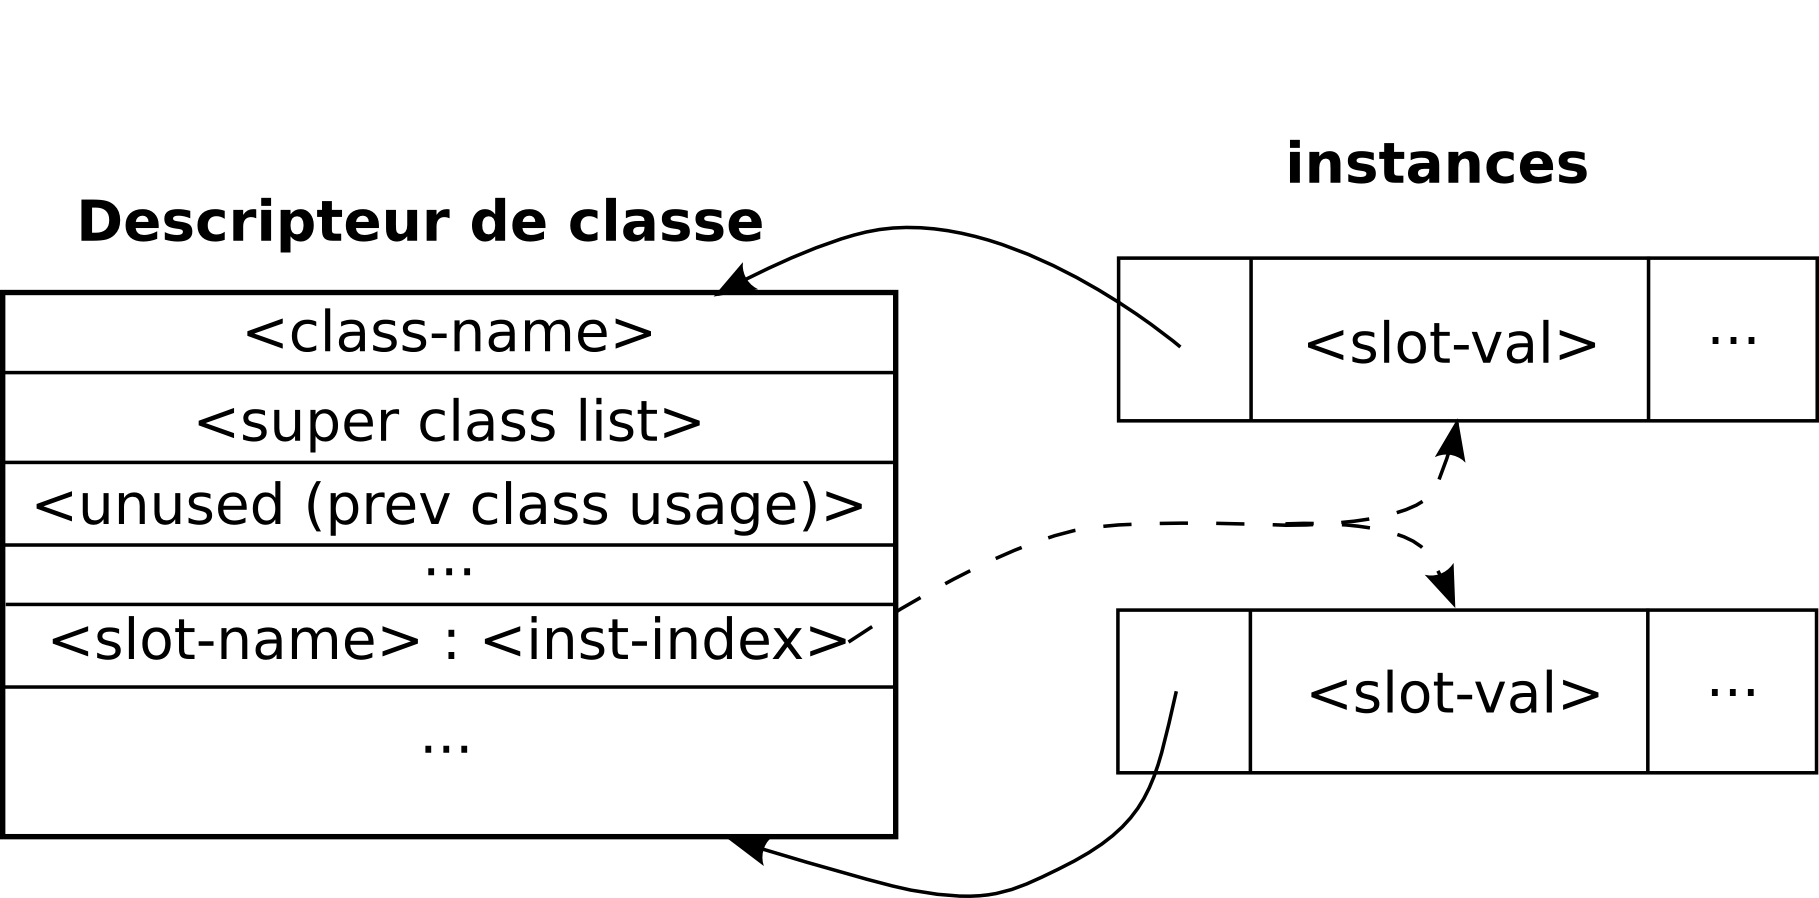
\includegraphics[scale=0.7]{oo-schema}
  \caption{Schématisation des structures créées dans la figure
    \ref{OO:obj-struct}}
  \label{OO:classdesc}
\end{figure}

Il aurait été possible de faire en sorte que ces index soient toujours
au même endroit pour une hiérarchie de classe donnée, mais nous avons
simplifié le problème dans notre implantation. En effet, les index
d'indirection se retrouvent au même endroit dans le descripteur de
classe, peu importe la classe. La conséquence de cette simplification
est que la taille des nouveaux descripteurs de classe augmente
linéairement en fonction du nombre d'attributs qui ont été déclarés
pour les classes précédemment définies. Une autre possibilité aurait
été de toujours placer les attributs au même endroit dans les
instances. Puisqu'en général peu de classes sont utilisées en
comparaison à la quantité d'instances créées, le choix effectué est un
bon compromis entre l'utilisation de la mémoire et la rapidité d'accès
aux attributs. Ces structures de données sont implantées en utilisant
des vecteurs \Schemelang. Ceux-ci ont été choisis dans le but de
donner un accès rapide aux attributs.

Lorsque la forme spéciale \scheme{define-class} est expansée,
plusieurs informations sont extraites et traitées afin de générer
correctement les fonctions de création et d'accès aux attributs. Entre
autres, il faut obtenir la liste complète de tous les attributs
hérités par les classes parents à la classe définie. Cette information
est stockée dans une table de hachage globale à l'expansion macro
nommée \scheme{mt-class-table} qui conserve l'information disponible
pour chaque classe déjà créée. Cette information, stockée sous forme
de méta descripteurs de classe, n'est disponible que pour l'expansion
macro. Ces descripteurs gardent une trace du nom des classes créées,
de leur hiérarchie et une liste de positions relatives aux
descripteurs de classes présents durant l'exécution. Ces positions
relatives indiquent où trouver les index d'indirection associés à
leurs attributs.

Lorsque les nouveaux attributs (non-hérités) sont inclus dans un
descripteur de classe de l'exécution, un compteur global (expansion
macro) est utilisé pour obtenir la position du nouveau champs dans le
vecteur correspondant à ce descripteur. Une fois toutes les positions
déterminées, la génération du descripteur de classe de l'exécution
peut être entamée. Un deuxième index, local celui-ci, est utilisé pour
trouvé l'index d'indirection des attributs dans l'instance. Ainsi,
l'index global pointe vers l'endroit où placer l'index d'indirection
des attributs d'instance dans le descripteur de classe de l'exécution.
Pour leurs parts, les index d'indirection indiquent où trouver les
attributs dans les instances. 

Une fois cette information en main, toutes les fonctions d'accès et de
modification d'attributs peuvent être générées sans problème. La
plupart contiendront des indirections pour l'accès aux champs, sauf
pour les attributs de classe qui eux, se retrouvent directement dans
les descripteurs de classe. La figure \ref{OO:slot-access} donne un
exemple concret de code généré effectuant l'accès au champs \scheme{x}
de la classe \scheme{point} définie dans la figure
\ref{OO:obj-struct}. Au total, trois indirections sont nécessaires à
l'obtention de la valeur d'un attribut d'instance. La première
indirection obtient le descripteur de classe de l'instance en
question. La deuxième cherche dans ce descripteur l'index
d'indirection qui donnera la position de l'attribut dans
l'instance. Puisque la position de cet index d'indirection est
globale, elle est directement insérée dans le code généré. Dans cette
exemple, cette position se trouve à l'index $2$ dans le descripteur de
classe. Finalement, la valeur de l'attribut est obtenue en effectuant
l'indirection sur l'instance.


\begin{figure}[htb!]
  \begin{verbatim}
(lambda (#:obj518)
  (vector-ref #:obj518 
              (vector-ref (instance-class-descriptor #:obj518) 
                          2)))
  \end{verbatim}
  \caption{Code généré pour l'accès à l'attribut \scheme{x} de la
    classe \scheme{point} de la figure \ref{OO:obj-struct}}
  \label{OO:slot-access}
\end{figure}

Deux constructeurs d'instances sont aussi générés. Le premier
(\scheme{make-<class-name>}) construit et initialise \emph{tous} les
champs d'une instance de la même manière que procède le constructeur
d'instance pour la forme \scheme{define-type} de Gambit-C. Le deuxième
(\scheme{make-<class-name>-instance}) ne prend aucun argument et
produit une instance non-initialisée qui pourra être passée à
\scheme{init!}, la fonction générique d'initialisation d'objets. Par
défaut, une instance de cette fonction générique est créée, et fait
exactement le même travail que le premier constructeur. De plus, une
fonction très rudimentaire d'introspection d'instance de classe est
implantée sous la forme d'instances de la fonction générique
\scheme{describe}.

Les choix d'implantation qui viennent d'être énumérés ont été faits
dans le but d'obtenir un compromis entre la rapidité du système et la
puissance expressive auquel il donne accès. Par exemple, on constate
qu'une indirection est faite sur une instance afin d'obtenir son
descripteur de classe, tandis qu'un pointeur vers ce descripteur de
classe aurait pu être placé directement (voir la figure
\ref{OO:slot-access}). Par contre, si un pointeur s'était retrouvé
directement dans la fonction d'accès \scheme{point-x}, il n'aurait
alors plus été possible de l'utiliser de manière polymorphique avec
les sous-classes de la classe \scheme{point} puisqu'il n'est pas
certain que l'attribut \scheme{x} se retrouvera au même endroit dans
une instance de ces sous-classes. Puisqu'un accès aux champs d'un
vecteur est une opération efficace en \Schemelang, nous avons préféré
opter pour la présence du polymorphisme qui apporte beaucoup en termes
d'expressivité.

Puisque le système objets est implanté en utilisant l'expanseur de
macros \scheme{define-macro} de Gambit-C, les données conservées sur
les classes définies durant cette expansion sont perdues lorsque
celle-ci est terminée. Par conséquent, il n'est pas possible de
modifier la hiérarchie de classe définie dans un module \Schemelang
(un fichier) à l'intérieur d'un autre module. Par exemple, une classe
\scheme{Alpha} définie dans un fichier \scheme{A} ne pourrait pas être
sous-classée dans un autre fichier \scheme{B}. Toutefois, il est
possible d'utiliser les hiérarchies de classes créées dans un premier
module à l'intérieur d'un autre module. L'implantation du support
intermodulaire du système objets n'a pas été abordée dû à la
complexité de la tâche et à la potentielle baisse de performance qui
pourrait découler d'un tel ajout.

\FloatBarrier
\subsection{Implantation de define-generic}
De manière similaire à la définition de nouvelles classes, des
informations sur les fonctions génériques définies et sur leurs
instances sont conservées dans une table de hachage globale durant
l'expansion macro et se nomme \scheme{mt-meth-table}. Ces informations
seront par la suite transférées vers l'exécution du programme sous la
forme de structures propres à chaque fonctions génériques qui se
nomment \scheme{<genfun-name>-meth-table}. Ces structures contiennent
le nom de la fonction générique, une table de hachage permettant de
vérifier rapidement l'existence d'une instance et une liste
\emph{triée} des instances permettant d'accélérer le polymorphisme de
fonctions génériques. La clé de cette table de hachage est basée sur
le type des arguments de l'instance stockée.

L'expansion de la définition d'une nouvelle fonction générique résulte
donc en la création de cette structure et d'une fonction portant le
nom de la fonction générique, qui a pour but de faire le choix de la
bonne instance à partir des paramètres qui lui sont passés. La
fonction de \textit{dispatch} générée pour la fonction générique
\scheme{init!} est illustrée dans la figure \ref{OO:init!-gf}. Le code
présenté a été légèrement modifié afin d'illustrer uniquement
l'essence du \textit{dispatch} effectué. On constate que dans un
premier temps, on cherche dans la table de hachage de cette fonction
générique si une instance associée aux types des arguments passés (ou
du \textit{cast} effectué) existe. Si ce ne pas le cas, on cherche
explicitement une instance admissible de manière polymorphe à ces
arguments.

\begin{figure}[htb!]
  \begin{schemecode}
(lambda (\#!key cast . args)
  (let ((types (cond ((pair? cast) cast) 
                     (else (map get-class-id args)))))
    (cond
      ((or (generic-function-get-instance init!-meth-table types))
           (find-polymorphic-instance? init!-meth-table 
                                       args types))
           => (lambda (method) 
                (apply (method-body method) args)))
      (else (error ...)))))
  \end{schemecode}
  \caption{Code expansé effectuant le \textit{dispatch} dynamique pour
    la fonction générique \scheme{init!}}
  \label{OO:init!-gf}
\end{figure}


L'algorithme qui détermine quelle instance est la plus spécifique pour
un ensemble d'argument donné est simple: on cherche à trouver la
première instance dont chacun des types est considéré équivalent au
type des arguments actuels \emph{dans une liste triée} des instances
en fonction de leur spécificité. Le critère de spécificité est
déterminé par la profondeur dans la hiérarchie du type des arguments
de l'instance, \ie par la somme du nombre de classes parents pour
chacun des types des arguments passés. En ce qui concerne les types
spéciaux comme \scheme{match-value}, ces types sont considérés comme
étant très spécifiques et donc prioritaires à une simple
correspondance du type d'un objet. La figure \ref{OO:polymorphism}
illustre le code utilisé pour réaliser ce \textit{dispatch}
polymorphique.

\begin{figure}[htb!]
  \begin{schemecode}
(define (find-polymorphic-instance? genfun actual-params actual-types)
  (let ((args-nb (length actual-params))
        (sorted-instances (generic-function-sorted-instances genfun)))
    (exists (lambda (method)
              (equivalent-types? (method-types method)
                                 actual-params
                                 actual-types))
            (filter (lambda (i) (= (length (method-types i)) args-nb))
                    sorted-instances))))
  \end{schemecode}
  \caption{Implantation de la recherche d'instances polymorphiques
    d'une fonction générique}
  \label{OO:polymorphism}
\end{figure}

À un certain moment la fonction \scheme{call-next-method} avait été
implantée en utilisant le mécanisme de variables à portée dynamique de
Gambit-C. Par contre, l'exécution du corps des méthodes à l'intérieur
d'un environnement dynamique ralentissait l'exécution de celles-ci
d'un facteur d'environ 15\%. Par conséquent, l'implantation de cette
fonction a été abandonnée. En effet, celle-ci permet d'écrire des
corps de méthodes légèrement plus génériques, mais l'utilisation du
\scheme{cast} permet de faire sensiblement le même travail sans avoir
à subir des pertes de performance.

\FloatBarrier
\subsection{Implantation de define-method}
L'expansion de la macro \scheme{define-method} consiste en la création
d'une structure de donnée qui contient le corps de l'instance définie
ainsi que les types associés aux arguments attendus. Cette structure
existera durant l'expansion et sera recréée lors de l'exécution du
programme afin d'être appelée par la fonction de \textit{dispatch}.


\FloatBarrier
\section{Performances} \label{OO:bench-sect}
Ce système de programmation orienté objets a été écrit dans le but
d'obtenir un compromis entre l'accès à des concepts de haut niveau et
de bonnes performances lors de l'exécution, notamment en ce qui
concerne l'accès aux membres d'instances de classes.

Dans un premier temps, les performances du système sont analysées de
manière théorique. Le tableau \ref{OO:complexity} donne la complexité
algorithmique des opérations utilisées. La création d'instances
directes, \ie utilisant les fonctions \scheme{make-<class-name>},
s'effectue en temps constant puisqu'il ne s'agit que de la création
d'un vecteur. Par contre, la création d'instances par des
constructeurs, \ie en utilisant \scheme{(new <class-name> ...)},
possède la complexité des appels de fonctions génériques directs. Par
\og appel direct \fg, il est sous-entendu que le type des arguments de
l'appel correspond aux types des arguments formels, et non de manière
polymorphe. Ces appels possèdent une complexité algorithmique linéaire
en fonction du nombre de paramètres que possède l'instance (appelons
le $p$). En effet, l'obtention d'une instance directe est faite par
l'entremise d'une recherche dans une table de hachage utilisant
\scheme{equal?} à titre de comparaison. Cette complexité augmente d'un
ordre supplémentaire lorsqu'aucune instance directe n'existe et qu'une
instance polymorphique est recherchée. En effet, une recherche
linéaire est effectuée sur chacune des instances existantes ($m$),
puis la compatibilité du type des arguments doit être effectué
($p$). Il est intéressant de noter que malgré la complexité
quadratique de cette opération, le nombre de paramètres ($p$) est
normalement très bas.  L'accès et la modification de membres de classe
se fait toutefois de manière constante.

\begin{table}
  \center
  \begin{tabular}{cc}
    \hline
    opération & complexité algorithmique \\
    \hline \hline
    création d'instances directe & $O(1)$\\
    création d'instances avec constructeurs & $O(p)$\\
    accès aux membres & $O(1)$ \\
    modification de membres & $O(1)$ \\
    \textit{dispatch} direct & $O(p)$\\
    \textit{dispatch} polymorphique & $O(mp)$\\
    \hline
  \end{tabular}
  \caption{Complexité algorithmique des opérations du système objets
    effectuées durant l'exécution}
  \label{OO:complexity}
\end{table}

Une comparaison pratique de performance a été effectuée avec d'autres
systèmes objets disponibles pour Gambit-C afin de mieux connaître les
constantes cachées dans la complexité des opérations effectuées durant
l'exécution. Il est aussi intéressant de comparer les performances du
système par rapport aux autres afin de confirmer l'obtention du
résultat désiré. Ces résultats sont présentés dans le tableau
\ref{OO:bench}. Ces derniers correspondent aux temps nécessaires à $1
000 000$ d'exécutions de chacune des opérations principales du système
objets. Les systèmes objets Meroon~\cite{MEROON}, OOPS~\cite{OOPS}
ainsi que les objets obtenus avec l'utilisation de la forme spéciale
\scheme{define-type} de Gambit-C ont été utilisés pour effectuer cette
comparaison. Le tableau \ref{OO:bench-rel} présente ces résultats
d'une manière relative au meilleur temps d'exécution du test pour
chaque opération vérifiée.

\begin{table}
  \center
  \begin{tabular}{ccccc}
    \hline
    Opération & define-type & Meroon & OOPS & class \\
    \hline \hline
    Création d'instances directes           & 0.005 & 0.215 & 1.423 & 0.007\\
    Création d'instances avec constructeurs & ND    & ND    & ND    & 2.173\\
    Accès aux membres                       & 0.006 & 0.126 & 3.120 & 0.014\\
    Modification de membres                 & 0.008 & 0.117 & 3.961 & 0.011\\
    \textit{Dispatch} direct                & 0.185 & 0.188 & 19.210 & 1.860\\
    \textit{Dispatch} polymorphique         & 0.213 & 0.773 & 18.995 & 5.786\\
    \hline
  \end{tabular}
  \caption{Temps d'exécution (en secondes) de $1 000 000$ d'itérations
    de tests comparatifs sur les opérations du système de
    programmation orientée objets développé avec d'autres systèmes
    objets existants}
  \label{OO:bench}
\end{table}

\begin{table}
  \center
  \begin{tabular}{ccccc}
    \hline
    Opération & define-type & Meroon & OOPS & class \\
    \hline \hline
    Création d'instances directes & 1.0 & 43.0 & 284.6 & 1.4 \\
    Création d'instances avec constructeurs & ND & ND & ND & 1.0 \\
    Accès aux membres & 1.0 & 21.0 & 520.0 & 2.3 \\
    Modification de membres & 1.0 & 14.6 & 495.1 & 1.4 \\
    \textit{Dispatch} direct & 1.0 & 1.0 & 103.8 & 10.0 \\
    \textit{Dispatch} polymorphique & 1.0 & 3.6 & 89.1 & 27.1 \\
    \hline
  \end{tabular}
  \caption{Comparaison de performances relatives au système le plus
    rapide (1.0) pour chaque opération du système objets.}
  \label{OO:bench-rel}
\end{table}

Ces résultats démontrent bien que les objectifs d'implantation ont été
atteints. En effet, le système développé (\scheme{class}) offre de
bonnes performances quant à la création d'instances et la manipulation
des membres de celles-ci. Malgré le fait que le système est environ un
ordre de grandeur plus lent que le système Meroon pour effectuer le
\textit{dispatch} dynamique de fonctions génériques, celui-ci offre
beaucoup plus d'expressivité dont l'utilisation de constructeurs ou de
discrimination sur des valeurs. Ainsi, le système développé offre
plusieurs concepts de haut niveau quant à la programmation orientée
objets et se compare aux autres systèmes d'objets performants
disponibles pour Gambit-C.

\FloatBarrier
\section{Conclusion}
Ainsi un système objets complet a été développé dans le but d'étendre
le langage \Schemelang et d'y inclure le paradigme de la programmation
orientée objets. Ce système objets permet la déclaration de classes avec
héritage multiple, polymorphisme et fonctions génériques effectuant du
\textit{dispatch} multiple. Ces choix de caractéristiques ont été
faits dans le but de donner le plus de liberté aux programmeurs de
jeux vidéo, tout en fournissant de bonnes performances, tant en temps
sur processeur qu'en utilisation de la mémoire.

Dans ce but, les structures de données utilisées pour l'implantation
d'instances de classe ne possèdent pas d'espaces inutilisés et ne
requièrent que trois indirections vectorielles afin d'accéder aux
champs de celles-ci. De même, les fonctions génériques utilisent des
mécanismes de tri pré-calculé afin d'accélérer le \textit{dispatch}
d'instances de fonctions génériques de manière polymorphe.

Il serait maintenant intéressant de modifier le système afin qu'il
supporte un protocole de méta objets. Un tel protocole donnerait accès
à une introspection très développée et permettrait aux utilisateurs de
modifier le comportement du système selon leurs besoins.

Aussi, une modification du système afin de le rendre compatible avec
des classes de manière inter-modulaire serait une grande amélioration
en ce qui concerne la modularité du code.

Par contre, une attention particulière devrait être portée aux coûts
en performance que ces modifications pourraient impliquer afin de
respecter la philosophie de base de ce système objets.

\clearpage

%%%%%%%%%%%%%%%%%%%%%%%%%%%%%%%%%%%%%%%%%%%%%%%%%%%%%%%%%%%%%%%%%%%%%%%%%%%%%%%
\chapter{Système de coroutines} \label{Chap:corout}
Les \textit{threads} constituent un outil de programmation important
permettant l'exécution parallèle matérielle ou logicielle de
code. L'utilisation de \textit{threads} dans un jeu vidéo peut être
très pertinente et permettrait d'exprimer de manière concise beaucoup
de concepts clés. Par exemple l'implantation de parties multi-joueurs
où ces derniers jouent à tours de rôles se représente bien par un
modèle parallèle, puisqu'il s'agit vraiment de deux parties distinctes
qui sont jouées en même temps.

Le langage \Schemelang tel que décrit par le standard~\cite{R5RS} ne fourni
pas de système de \textit{threads}. Par contre, le document SRFI
18~\cite{SRFI18} (\textit{Scheme Request For Implementation}) décrit
un \textit{API} (\textit{Application Programming Interface}) de
système de \textit{thread} concurrents. Le système
Gambit-C~\cite{Gambit4} supporte cet \textit{API} sous forme de
\textit{threads} verts, \ie  sous formes de concurrence logicielle et
non matérielle. Malheureusement, le coût d'utilisation des mécanismes
de synchronisation explicites est très élevé en temps de développement
et en utilisation du processeur lors de l'exécution.

Par contre, un système de coroutines (appelé aussi \textit{threads}
coopératifs) permettrait d'éviter d'avoir à spécifier explicitement
ces synchronisations entre entités. En effet, si le flot de contrôle
est changé durant des moments opportuns connus du programmeur, aucune
synchronisation supplémentaire n'est requise pour assurer la validité
d'accès concurrents à des sections critiques. En fait, le problème ne
se pose même plus, mais disparaît complètement. Ceci rend donc très
attrayant de tels systèmes pour le développement de jeux vidéo. Il
permettrait d'exprimer de manière simple des changements de contextes
dans le jeu, ou même, de modulariser le comportement de chacune des
entités du jeu. Pour ce faire et afin de conserver la modularité du
jeu, on peut imaginer une cascade de systèmes de coroutines dont un
premier niveau permettrait l'implantation de parties multi-joueurs et
un second niveau permettrait l'implantation du comportement d'entités
dans le jeu. La figure \ref{Corout:usecase} illustre de manière
générique cette idée. Dans ce schéma, les carrés noirs représentent
des système de coroutines et les coroutines sont représentées avec des
lignes pointillées. L'utilisation systèmes imbriqués permettrait ainsi
d'exprimer chaque concept de manière modulaire de manière complètement
transparente.

\begin{figure}[htb!]
  \center
  \includegraphics[scale=1.2]{corout-usecase-design}
  \caption{Exemple générique d'utilisation de systèmes de coroutines
    cascadés}
  \label{Corout:usecase}
\end{figure}

Gambit-C offre la possibilité de transformer son système de
\textit{threads} en système de coroutines lorsque le délais de
changement de contexte automatique est choisi comme étant
l'infini. Toutefois, il est impossible d'utiliser plusieurs systèmes
de coroutines avec cette approche. Ainsi, l'utilisation directe des
fonctionnalités de Gambit-C limite l'utilisation de coroutines au
développement d'un seul concept dans un jeu.

Afin de ne pas être limité par les fonctionnalités fournies par
Gambit-C, l'expressivité du langage \Schemelang peut être mise à profit. En
effet, grâce à la réification de continuations du calcul, la tâche de
l'implantation d'un système de coroutine fait sur mesure est tout à
fait accessible et réalisable sans changer le langage. Ce chapitre
présente un système de \textit{threads} \emph{coopératifs} développé
dans le but de bien répondre aux besoins de jeux vidéo quant à
l'écriture de code s'exécutant en concurrente de manière sécuritaire
tout en permettant l'utilisation récursive de ce système.


\FloatBarrier
\section{Description du langage}
Un système de \textit{threads} coopératifs implique donc que le
changement de contexte d'exécution associés aux changements de
\textit{threads} doivent être faits de manière explicite par les
utilisateurs. Ainsi, ces changements de contextes peuvent être faits
aux moments opportuns, pour assurer l'intégrité des
données. Toutefois, des synchronisations entre les différentes
coroutines pourraient être encore nécessaires afin de bien orchestrer
l'exécution de ces dernières. Afin de permettre aux coroutines de
communiquer entre elles, une synchronisation par passage de message
avec \textit{pattern matching} similaire à celle utilisée dans les
systèmes Termite~\cite{Termite_paper} ou Erlang~\cite{Erlang} a été
adoptée. Ce mécanisme permet de synchroniser de manière élégante les
coroutines naturellement.

De plus, le système a été conçu pour être utilisé récursivement. Il
est donc possible d'avoir une coroutine qui sera elle-même un système
de coroutine, et ainsi de suite. Cette fonctionnalité a été implantée
pour que le système soit le plus générique possible. De plus, l'idée
de système récursifs est aussi très près du langage \Schemelang dans lequel
la récursion de fonctions est très courante et commune grâce à
l'implantation de l'optimisation d'appels terminaux.

Un tel système de coroutine peut être également vu comme étant un
système de simulation basée sur les agents, par opposition aux
simulations basées sur des événements discrets. Le comportement des
entités est alors représenté par chacune des coroutines du
système. Dans cette optique, la notion de temps du système développé a
été abstraite grâce à l'introduction de compteurs de temps
(\textit{timers}). Il est donc possible de choisir non seulement une
granularité temporelle en spécifiant la fréquence de ce compteur, mais
il est aussi possible de spécifier un facteur d'accélération,
permettant d'accélérer la simulation en cours.

Le système se résume à un ordonnanceur de coroutine qui utilise une
file de coroutines prêtes à exécuter pour choisir la prochaine qui
doit prendre le contrôle. Aussi, une file de coroutines en attente sur
le temps et sur des conditions sont disponible pour une bonne
régulation du système. Lorsqu'une coroutine décide de passer la main à
la coroutine suivante ou lorsqu'elle ne doit plus attendre après le
temps ou une condition, elle se fait enfiler à la fin de la file
d'attente de coroutines prêtes. La figure \ref{Corout:system-schema}
illustre l'architecture globale du système.

\begin{figure}[htb!]
  \center
  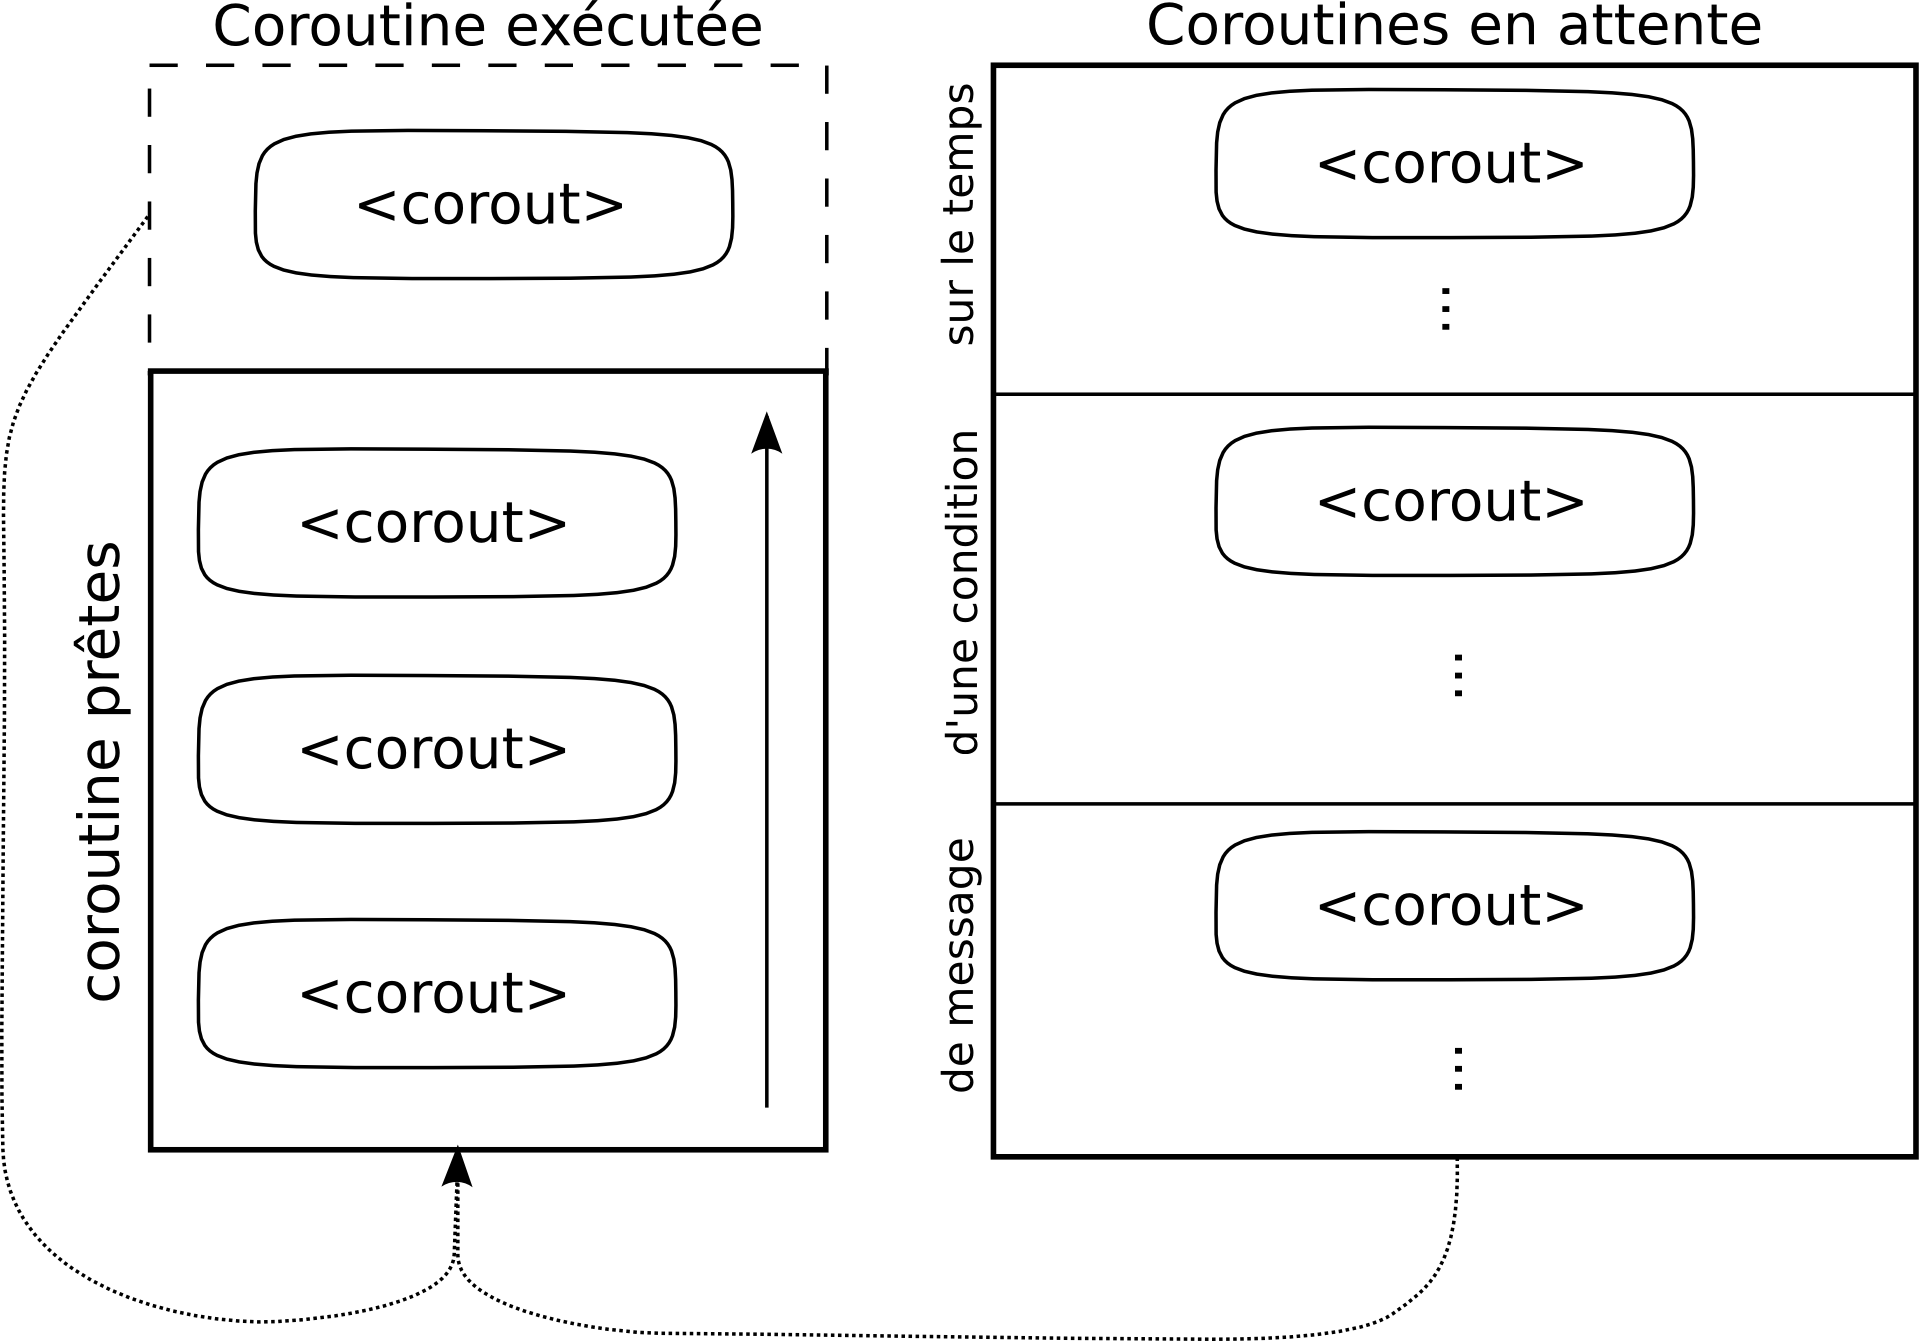
\includegraphics[scale=0.7]{corout-system}
  \caption{Architecture globale du système de coroutine}
  \label{Corout:system-schema}
\end{figure}

 Les sections suivantes décrivent un \textit{API} permettant
l'utilisation du système de coroutines développé.


\FloatBarrier
\subsection{Création de coroutines}
Les coroutines sont des objets en eux même et peuvent être créés de
manière externe au système de coroutines pour, par la suite, être
ajoutées à celui-ci. L'avantage de cette approche, utilisée aussi par
le système de \textit{threads} de Gambit-C, réside dans le fait que
les objets correspondant aux \textit{threads} peuvent être initialisés
à l'avance et conservés jusqu'au moment opportun de leurs ajout au
système. Une nouvelle instance de coroutine s'effectue avec

\begin{schemecode}
(new-corout <corout-id> <thunk>)
\end{schemecode}

\noindent
où \scheme{<corout-id>} est un symbol permettant d'identifier la
coroutine et le dernier argument est un \textit{thunk} (une fonction
ne prenant aucun argument) qui contient le corps de l'exécution de
cette coroutine.

La figure \ref{Corout:state-diag} illustre un diagramme des états
possibles pour une coroutine avec les transitions correspondantes. Sur
chacune des transition, un exemple d'appel de fonction effectuant
cette transition est donné. On constate ainsi qu'une coroutine est
soit prête, en attente ou bien terminée. L'attente d'une coroutine
peut être conditionnelle à la réception d'un message, au relâchement
d'une sémaphore ou à un certain délais de temps prescrit. De plus,
l'attente sur le temps peut être interruptible par la réception d'un
message. Cet état se produit lorsqu'une attente de message est
effectuée avec une attente bornée.

\begin{figure}[htb!]
  \center
  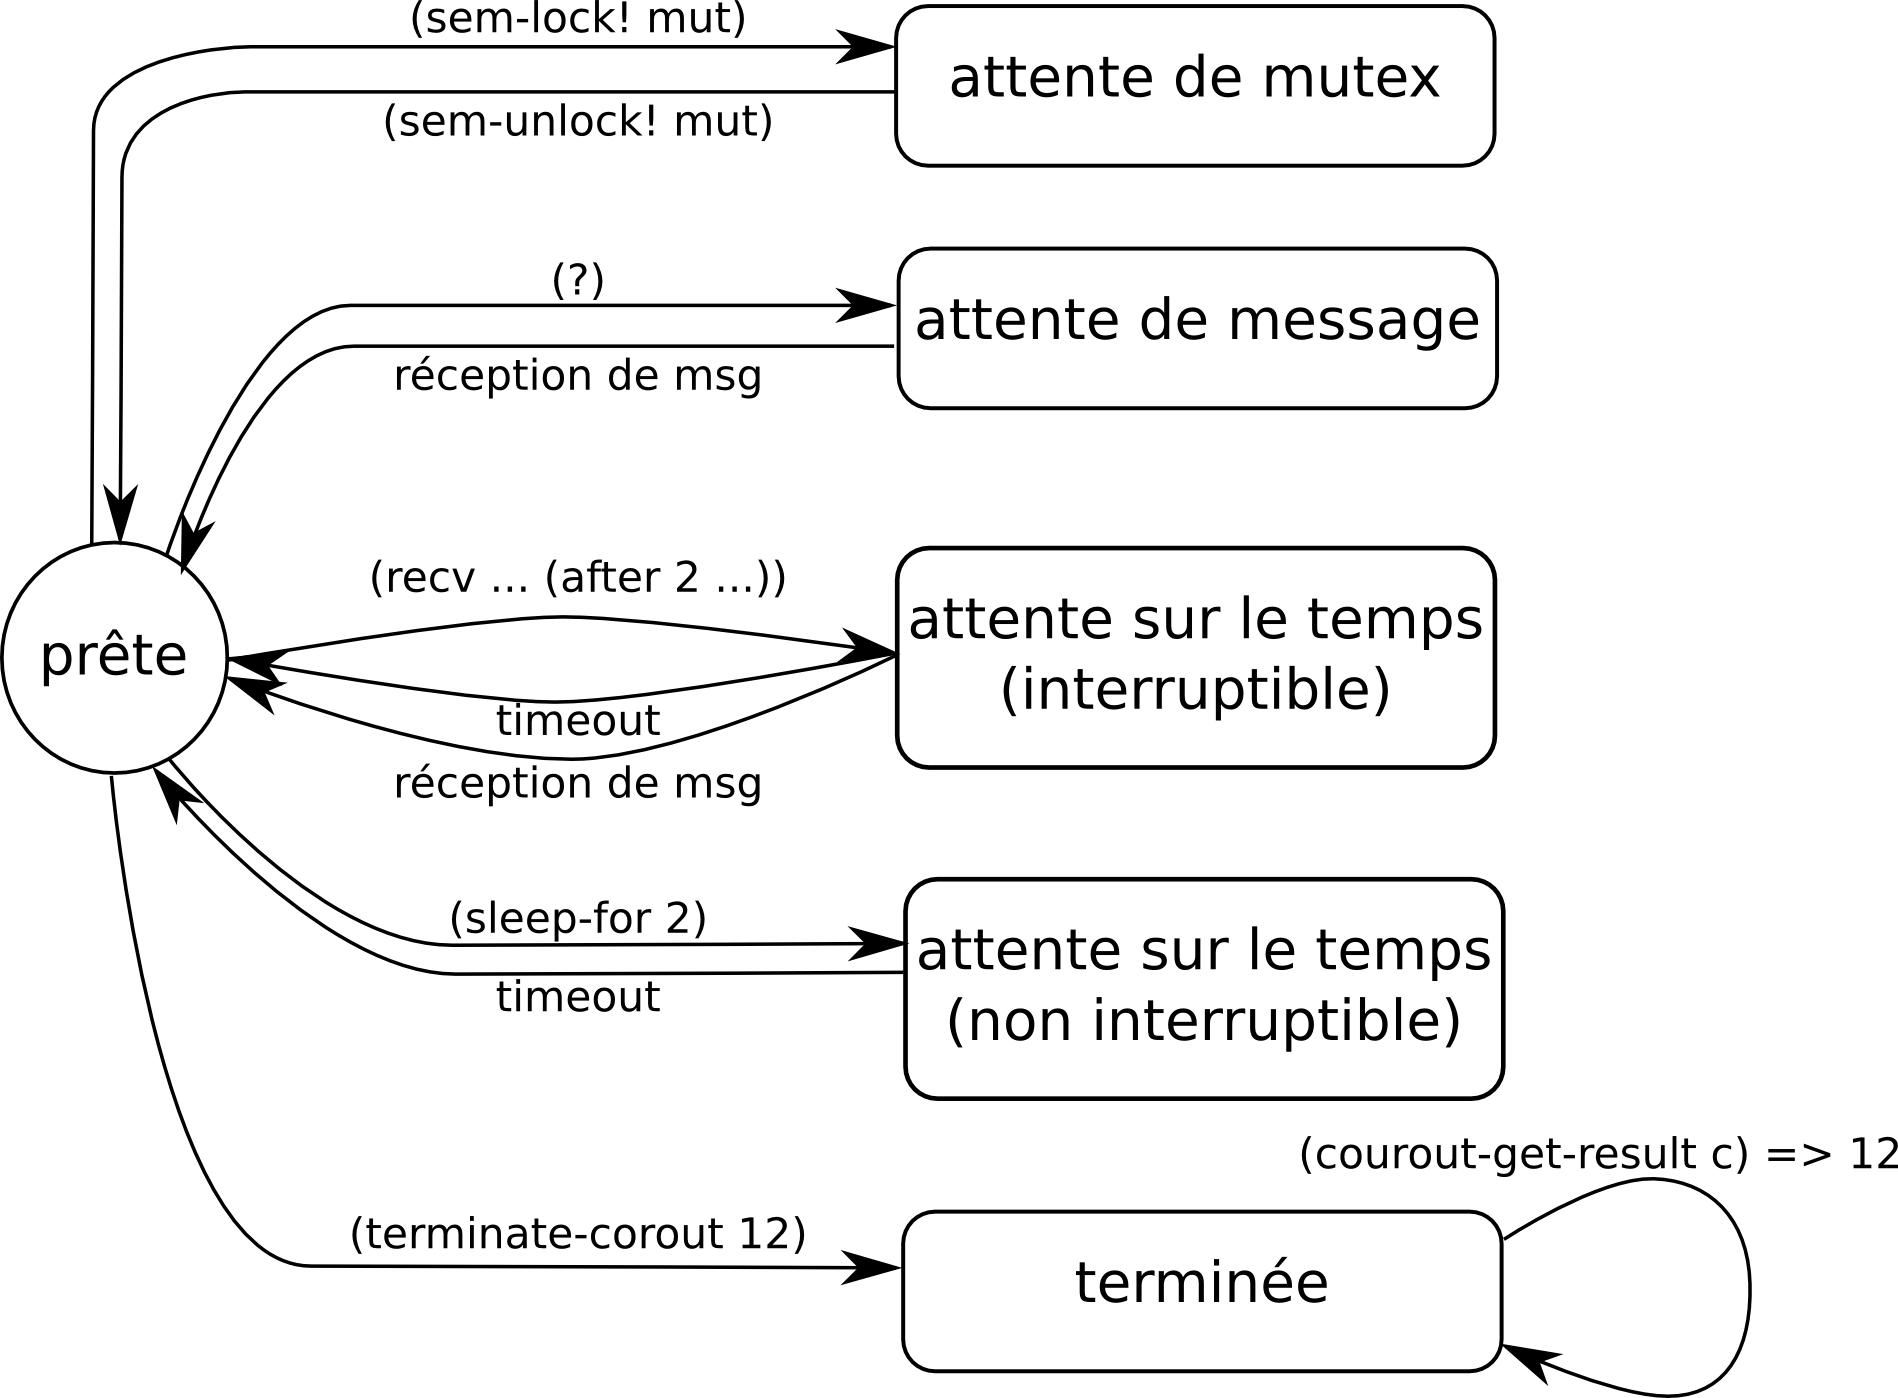
\includegraphics[scale=0.6]{corout-state-diag}
  \caption{Diagramme d'états d'une coroutine}
  \label{Corout:state-diag}
\end{figure}

L'objet créé pourra être par la suite ajouté à un nouveau système par
la fonction d'initialisation \scheme{boot} ou encore par une coroutine
d'une simulation existante avec la fonction
\scheme{spawn-brother}. Ces fonction sont décrites ci-dessous.


\FloatBarrier
\subsection{Démarrage du système}
Le système de coroutines peut être démarré en utilisant la fonction 

\begin{schemecode}
(boot <list of corout> [<timer>])
\end{schemecode}

\noindent
dont le premier argument doit être une liste contenant les coroutine
présentes lors du démarrage du système et, optionnellement un objet
correspondant à un compteur de temps pour le système. L'ordre des
coroutines dans la liste est significatif car il indique dans quel
ordre seront enfilées les coroutines dans la file d'attente de
coroutines prêtes. Ainsi, la première coroutine de la liste sera la
première à être exécutée. La création de \textit{timers} se fait par
un appel à la fonction

\begin{schemecode}
(start-timer! <period> [time-multiplier: <time-mult-value>]))
\end{schemecode}

\noindent
qui s'occupe de créer un objet faisant abstraction du temps. Ce
dernier sera rafraîchi selon la période (en seconde) indiquée en temps
réel. On peut ainsi faire varier la granularité de la simulation afin
de l'adapter aux besoins existant. Le paramètre optionnelle
\scheme{<time-mult-value>}, si spécifié, accélérera la simulation de
ce facteur. Ainsi, le temps dans la simulation passera deux fois plus
vite que le temps réel en utilisant une valeur de multiplicateur de
temps de deux. La fonction \scheme{(pause-timer! <timer>)} peut être
utilisée afin de mettre en pause et de repartir le compteur de temps.

La figure \ref{Corout:boot} présente un exemple de démarrage d'un
système de coroutine où le temps sera augmenté toutes les secondes et
où le résultat final de la simulation sera la somme des valeurs
retournées par chacune des coroutines. Il est important de noter qu'il
ne faut pas oublier d'arrêter le \textit{timer} lorsqu'il n'est plus
nécessaire.

\begin{figure}[htb!]
  \begin{schemecode}
(let* ((c1 (new-corout 'c1 (lambda () (display 1))))
       (c2 (new-corout 'c2 (lambda () (display 2))))
       (c3 (new-corout 'c3 (lambda () (display 3))))
       (timer (start-timer! 1.0)))
  (boot (list c1 c2 c3))) => \schemeresult{123}
  \end{schemecode}
  \caption{Exemple de démarrage d'un système de coroutines}
  \label{Corout:boot}
\end{figure}

Le système de coroutine a été conçu de manière à permettre de créer
des systèmes de coroutines de manière cascadée, \ie de créer des
coroutines qui sont elles-mêmes des systèmes de coroutines. De tels
systèmes récursifs comportent de nombreux avantages. En effet,
l'utilisation de tels systèmes facilite grandement la modularité de
l'utilisation du système de coroutine. En effet, il devient possible
de modulariser les différents aspects d'utilisations dans leurs
propres systèmes. Par exemple, dans le cadre de jeux simples, on peut
implanter des parties multi-joueurs en utilisant une coroutine par
partie. Ces coroutine peuvent alors elle-même contenir un système de
coroutine utilisé par la partie en elle-même.

La procédure de création de ces derniers est simple, il suffit de
démarrer un nouveau système de coroutine à l'intérieur d'une coroutine
existante. Lorsque des coroutines démarrent un nouveau système de
coroutines, l'objet d'abstraction du temps (\textit{timer}) du système
de coroutine primordial est automatiquement utilisé pour les systèmes
récursifs de manière à conserver une cohérence entre ceux-ci. Par
contre, un problème se pose: il devient alors impossible de pouvoir
retourner le contrôle aux coroutines appartenant au système
primordial, puisque \scheme{(yield)} ne fera que changer de contexte
que les coroutines du sous-système.

Ce problème est résolu par l'utilisation de la fonction
\scheme{(super-yield)} qui effectue un changement de contexte pour le
système de coroutine courant. Si le système courant ne se retrouve pas
dans un système cascadé, alors rien ne se produira. Une fonction
similaire, \scheme{(super-kill-all! <return-value>)} terminera
\emph{tous} les systèmes de coroutines se retrouvant dans
l'arborescence de système de coroutine présentement active. Un exemple
de système de coroutines en cascade est donné dans la figure
\ref{Corout:cascade}.  On constate que les appels à
\scheme{super-yield} ont bien effectué les changements de contextes de
des coroutines hôtes des sous-systèmes de coroutines (\scheme{s1} et
\scheme{s2}).

\begin{figure}[htb!]
  \begin{schemecode}
(let* ((ret (lambda (x) (pp `(now returning: ,x)) x))
       (c1 (new-corout 'c1 (lambda () (ret 1))))
       (c2 (new-corout 'c2 (lambda () (super-yield) (ret 2))))
       (c3 (new-corout 'c3 (lambda () (super-yield) (ret 3))))
       
       (c4 (new-corout 'c4 (lambda () (ret 4))))
       (c5 (new-corout 'c5 (lambda () (super-yield) (ret 5))))
       (c6 (new-corout 'c6 (lambda () (ret 6))))
       
       (s1 (new-corout 's1 (lambda () (boot (list c1 c2 c3)))))
       (s2 (new-corout 's2 (lambda () (boot (list c4 c5 c6))))))
  (boot (list s1 s2))
  (fold-l + 0 (map corout-get-result (list c1 c2 c3 c4 c5 c6))))
=> \schemeresult{(now returning: 1)}
   \schemeresult{(now returning: 4)}
   \schemeresult{(now returning: 2)}
   \schemeresult{(now returning: 5)}
   \schemeresult{(now returning: 6)}
   \schemeresult{(now returning: 3)}
   \schemeresult{21}
  \end{schemecode}
  \caption{Exemple de démarrage de système de coroutines en cascade}
  \label{Corout:cascade}
\end{figure}


\FloatBarrier
\subsection{Manipulation du flot de contrôle}
Puisque le contrôle du flot d'exécution entre les coroutines doit être
explicité par l'utilisateur, une bonne diversité de fonctions
permettent la manipulation de celui-ci. Il est important de noter que,
sauf avec avis contraire, toutes les fonctions décrites dans cette
section doivent être exécutée \emph{par} une coroutine, \ie dans leur
corps.

La fonction la plus simple de manipulation du flot d'exécution est
\scheme{(yield)}. Celle-ci arrête temporairement la coroutine actuelle
et passe le contrôle à la \emph{prochaine} coroutine disponible. Cette
dernière est déterminée en utilisant la prochaine coroutine présente
dans la file de coroutines prêtes, tel qu'illustré dans la figure
\ref{Corout:system-schema}. La coroutine effectuant l'appel à la
fonction \scheme{yield} sera alors placée à la fin de cette file
d'attente. Il en résulte que le retour du contrôle à cette coroutine
ne sera exécutée uniquement lorsque toutes les autres coroutines
prêtes auront décidée de passer la main à la coroutine suivante. Il
est également possible de choisir explicitement à quelle coroutine le
contrôle sera passé avec la fonction \scheme{(yield-to <corout>)}.

Une coroutine peut aussi décider de se mettre en attente pour une
certaine période de temps avec la fonction \scheme{(sleep-for <sec>)}
un certain nombre de secondes. Il en résultera que la coroutine
actuelle sera placée dans une file d'attente séparée et ne sera
réenfilée dans la file de coroutines prêtes uniquement lorsque le
délais prescrit sera dépassé. Cela n'implique pas que la coroutine
sera exécutée à ce moment là, car si cette file contient déjà des
coroutines en attentes, elle devra attendre son tour pour poursuivre
son exécution. Puisqu'une telle attente peu varier en fonction de la
plate-forme utilisée, elle introduit un certain indéterminisme dans le
système.

Il est également possible pour une coroutine d'ajouter de nouvelles
coroutines dans le système en utilisant les fonctions:

\begin{schemecode}
(spawn-brother <corout>)
(spawn-brother-thunk <corout-id> <thunk>)
\end{schemecode}

La première ajoute simplement la coroutine spécifiée dans la file de
coroutines prêtes. Cette coroutine \emph{ne doit pas} déjà être
présente dans le système. La deuxième fonction,
\scheme{spawn-brother-thunk}, sert de sucre syntaxique en créeant une
nouvelle coroutine ayant comme identificateur \scheme{<corout-id>} et
la fonction spécifiée comme corps avant d'ajouter cette dernière dans
le système.

Dans le cadre de l'écriture de jeux vidéo, la modularité des
coroutines est très importante. Afin de faciliter l'écriture modulaire
de corps des coroutines, des formes spéciales permettant d'utiliser un
style CPS ont été ajoutées. Ces dernière permettent l'altération le
fil d'exécution d'une coroutine en modifiant la continuation de son
calcul par celui d'une autre coroutine ou d'un \textit{thunk}. Ainsi,
un appel à la forme spéciale \scheme{(continue-with <corout>)} fera en
sorte que la continuation de la coroutine devienne celle de cette
autre coroutine. De manière similaire, \scheme{(continue-with-thunk!
  <thunk>)} utilisera la fonction passée comme continuation du
calcul. La figure \ref{Corout:cont-mod} présente un exemple utilisant
ces deux formes spéciales. Lorsque la coroutine \scheme{c1} s'exécute,
sa continue change pour celle de \scheme{c2} qui change à sont tour
pour la fonction \scheme{t}. Ainsi, la fin du corps des coroutines
\scheme{c1} et \scheme{c2} ne sera jamais exécutée puisque leurs
continuation ont été altérées.

\begin{figure}[htb!]
  \begin{schemecode}
(let* ((t (lambda () (pp 'bonjour)))
       (c2 (new corout 'c2
                (lambda () (continue-with-thunk! t) (pp 'allo ) 2)))
       (c1 (new corout 'c1
                (lambda () (continue-with c2) (pp 'salut) 1))))
  (boot (list c1))) => \schemeresult{bonjour}
  \end{schemecode}
  \caption{Exemple de modification de la continuation d'une coroutine}
  \label{Corout:cont-mod}
\end{figure}

Finalement, une coroutine peut changer sa continuation de manière plus
drastique en forçant la terminaison du fil d'exécution de celle-ci en
utilisant la fonction \scheme{(terminate-corout <return-val>)}. La
valeur de retour de la coroutine spécifiée en paramètre est conservée
dans la structure de donnée de la coroutine et peut être obtenue en
faisant appel à la fonction \scheme{(corout-get-result <corout>)}. Il
est aussi possible de faire terminer le système actuel de coroutine,
au complet, en faisant appel à \scheme{(kill-all!  <return-val>)}. La
valeur de retour finale de l'exécution du système sera alors la valeur
spécifiée.


\FloatBarrier
\subsection{Environnement dynamique}
Une certaine introspection est très utile pour un programmeur, surtout
pour des fins de déboggage.  Un environnement dynamique est disponible
pour les coroutines, lors de leurs exécution. Cet environnement donne
accès à de l'information sur ce dernier. il comprend les paramètres:

\begin{itemize}
\item \scheme{(current-corout)} : retourne l'instance de la coroutine
  actuellement exécutée. 

\item \scheme{(timer)} : retourne l'objet d'abstraction du temps
  associé avec le système courant. La valeur actuelle du temps peut
  être obtenue en appellent plutôt la fonction
  \scheme{(current-sim-time)}.
\end{itemize}



\subsection{Système de communication inter-coroutines}
Que ce soit afin d'informer une partie du score d'un autre joueur ou
d'un vaisseau spatial attendant le bon moment pour effectuer son
déplacement la synchronisation des entités d'un jeu est primordiale.
Le mécanisme principal de synchronisation des coroutines pour ce
système est basé sur le passage de messages, tel que fait dans le
système de programmation distribué Termite~\cite{Termite_paper}. Cette
approche semble naturelle pour la programmation de jeux vidéo où les
coroutines peuvent devenir des entités à part entière et pourraient
ainsi communiquer avec d'autres entités par ces mécanismes d'une
manière naturelle.

L'envoi de messages se fait par la fonction \scheme{(! <corout>
  <msg>)} qui s'occupe d'acheminer le message désiré à la coroutine
spécifiée. La réception de messages, quant à elle, se fait avec deux
fonctions distinctes et une forme spéciale:

\begin{itemize}
\item \scheme{(? [timeout: <sec>])} : Réception du premier message
  disponible avec attente bloquante. Un \textit{timeout} peut être
  spécifié afin de limiter l'attente faite. Si plusieurs messages sont
  disponibles, le premier arrivé sera alors retourné.

\item \scheme{(?? <predicat> [timeout: <secs>])} : Réception du
  premier message qui retourne vrai selon le prédicat spécifié. Le
  prédicat doit prendre un seul argument, un message reçu. Comme pour
  la fonction \scheme{?}, l'attente bloquante peut être interrompue
  après un délai de temps, si ce dernier est spécifié.

\item \scheme{(recv (<pattern> <body>) ...)} : Cette forme spéciale
  permet la réception sélective de messages selon des patrons de
  filtrage par motifs (\textit{pattern matching}). Ces patrons
  permettent d'exprimer la forme attendue du message et de lier des
  variables locales à des parties du message reçu afin de les utiliser
  dans le corps du patron. Lorsque plusieurs messages reçus peuvent
  correspondre aux motifs donnés, la sélection du message se fait en
  choisissant le premier message reçu qui correspond à au moins un
  patron. Si plusieurs patrons peuvent correspondre à ce message, le
  premier patron (selon l'ordre de définition) sera utilisé. Ainsi
  l'ordre de spécification des motifs est important et significatif.
\end{itemize}

Les valeurs de délai d'attente maximal spécifié pour la réception de
messages implique qu'il est possible qu'une réception échoue. Dans un
tel cas, une exception de type \scheme{mailbox-timeout-exception} est
lancée par la fonction de réception utilisée.

Les patrons utilisés dans le filtrage de motifs de la forme spéciale
\scheme{recv} diffèrent de ceux dans Termite. Ici, le patron doit être
une donnée \Schemelang. Lorsque, dans cette donnée, un symbole est précédé
d'une virgule (\textit{unquote}), le symbole est \emph{lié} à la
valeur trouvée à cet endroit du motif dans le message reçu. Les
formats de motifs reconnus sont les symboles, les mots clés, les
caractères, les valeurs booléennes, les nombres, les chaînes de
caractères, les listes et les vecteurs. Aussi, il est possible
d'ajouter des gardes (filtrage conditionnel au prédicat) en incluant
une liste de la forme \scheme{(where <pred-expr>)} après le motif de
filtrage. Le prédicat utilisé est simplement une expression
\Schemelang. Finalement, un patron spécial permettant d'effectuer des
attentes bornées dans le temps est disponible sous la forme
\scheme{(after <timeout> <body> ...)}. Ce patron spécial doit être
spécifié \emph{en dernier}, s'il est présent. La figure
\ref{Corout:recv-pat} illustre plusieurs motifs différents qui peuvent
être utilisés.

\begin{figure}[htb!]
  \begin{schemecode}
(recv (salut                      'got-salut)      ; symbol match
      ("bonjour"                  'bonjour)        ; string match
      (1011                       '11-or-1011?)    ; number match
      ((a ,b c)                   (string b \#\textbackslash k)) ; list match
      (\#(a b ,c)                  c)               ; vector match
      (,any-char                                   ; guarded match
       (where (char? any-char))   'got-a-char)
      ((tata 1 \#(toto ,x) "titi")                  ; complex match
       (where (number? x))        (+ x 1))
      (,anything                  anything)        ; can match anything
      (after 2                    'timeout!))      ; timeout
  \end{schemecode}
  \caption{Exemple de patrons pouvant être utilisés dans le filtrage
    par motifs de la forme spécial \scheme{recv}}
  \label{Corout:recv-pat}
\end{figure}

Une particularité intéressante de ce filtrage par motif est reliée au
fait qu'il est possible d'utiliser des patrons de manière dynamique,
\ie qui n'apparaissent pas dans la forme spéciale \scheme{recv}, mais
plutôt qui ont été spécifiés grâce à une autre forme spéciale,
\scheme{(with-dynamic-handlers ((<pattern> <handler-body>) ...)
  <body>)}. Tous les appels à \scheme{recv} se trouvant dans le corps
(\scheme{<body>}) de \scheme{with-dynamic-handlers} se trouveront
augmentés de ces nouveaux patrons. Il est important de mentionné que
ces patrons dynamiques seront toutefois considérés en dernier lieu. Il
est donc possible de factoriser des patrons communs et de les
appliquer à tous les appels de la forme spéciale de réception de
messages par filtrage de motifs.

Le filtrage par patron présenté se conforme à la sémantique définie
par les formes équivalente dans les système Termite~\cite{Termite} et
Erlang~\cite{Erlang} par le fait que la sélection du message reçu se
fait sur le premier message reçu qui correspond à au moins un patron
de filtrage. Ce choix semble raisonnable puisqu'il en résulte que la
sélection de message est complètement déterministe. En effet, la
réception de nouveaux messages (qui est indéterministe dû à
l'incertitude qu'apporte la fonction \scheme{sleep-for}) n'influence
pas le choix du message. Si un message déjà reçu correspond à un
patron il sera choisi peu importe l'arrivée d'un nouveau message. Il
en découle que le système de messagerie est robuste et fiable.

Aussi, un mécanisme de liste de diffusion a été inclus. Ce mécanisme
simple permet d'enregistrer des coroutine dans une liste de diffusion
et, par la suite, d'envoyer à toutes les coroutines inscrites des
messages de manière simultanée. Quoi que très primitif, ce système
permet d'émuler la base d'un système de programmation
réactive~\cite{FRP}. Les fonctions de gestion et d'utilisation de
listes de diffusions sont:

\begin{itemize}
\item \scheme{(subscribe <list-id> <corout>)} : Inscription de la
  coroutine spécifiée à la liste de diffusion identifiée par le symbole
  choisi. Si la liste n'existait pas, elle sera créée.

\item \scheme{(unsubscribe <list-id> <corout>)} : Désinscription d'une
  coroutine à une liste de diffusion.

\item \scheme{(broadcast <list-id> <msg>)} : Envoi d'un message à une
  liste de diffusion.
\end{itemize}

\noindent
Un identificateur de liste de diffusion est représenté par une donné
\Schemelang. L'avantage d'utiliser des données comme identificateur est
qu'il est alors possible de créer celui-ci durant
l'exécution. L'utilisation de variables \Schemelang pointant vers une
structure de donnés, plutôt que des données \Schemelang, offriraient de
meilleurs performances, mais ce dynamisme ne serait pas disponible.


\FloatBarrier
\subsection{Autres mécanismes de synchronisation}
Le mécanisme de messagerie sophistiqué du système de coroutine permet
d'effectuer de manière élégante les synchronisation nécessaire entre
les coroutines. Toutefois, certains problèmes pourraient être exprimés
plus facilement grâce à des moyens plus traditionnels de
synchronisation.  Pour ce faire, des
sémaphores~\cite{DIJKSTRA_SEMAPHORE} ont été ajoutées au système de
coroutine développé. Celles-ci permettent donc d'exprimer de manière
différente les contraintes de synchronisations qui peuvent être
nécessaire pour l'implantation d'un jeu. Les fonctions de manipulation
et de création de sémaphores sont données ci-bas:

\begin{itemize}
\item \scheme{(new-semaphore <init-value>)} : Création d'une nouvelle
  sémaphore ayant comme valeur initiale \scheme{<init-value>}.

\item \scheme{(new-mutex)} : Création d'une nouvelle sémaphore ayant
  comme valeur initiale 1.

\item \scheme{(sem-locked? <sem>)} : Permet de vérifier s'il reste des
  ressources disponibles dans une sémaphore. S'il en reste, la
  fonction retournera vrai, et faux sinon.

\item \scheme{(sem-lock! <sem>)} : Prend une ressource de la sémaphore
  spécifiée. Si aucune ressource n'est disponible, la coroutine se met
  en état d'attente bloquante jusqu'à ce qu'une ressource soit
  libérée.

\item \scheme{(sem-unlock! <sem>)} : Libère une ressource de la
  sémaphore spécifiée. Aucune vérification n'est faite pour s'assurer
  que la coroutine courante possède réellement cette ressource. Si des
  coroutines sont en attentes de cette ressource, la première à s'être
  mise en attente est alors réveillée et enfilée dans la file de
  coroutines prêtes.
\end{itemize}



\FloatBarrier
\section{Implantation}
L'implantation de ce système de coroutine est centralisée sur
l'utilisation des fonctions \scheme{continuation-capture} et
\scheme{continuation-return} afin de permettre la conservation de
l'état courant d'une coroutine.

Un net avantage lorsque le système est directement implanté par
l'utilisateur est qu'il répond sur mesure aux demandes de ce dernier
et donc il peut s'exprimer dans une syntaxe simple, tout en conservant
un contrôle fin sur le comportement du système.

Cette section explique les mécaniques internes du système de
coroutines développé, en expliquant non seulement les structures de
données utilisées, mais aussi les algorithmes utilisés.

\FloatBarrier
\subsection{Implantation des coroutines}
La structure de donnée des coroutine est implantée en utilisant le
système d'objets fourni dans le système Gambit-C. Une version orientée
objet est aussi disponible. La structure employée est illustrée dans
la figure \ref{Corout:corout-class}. Elle contient toutes les
informations essentielles au fonctionnement de celle-ci, dont entre
autre sa continuation (\scheme{kont}), sa boîte de messagerie, une
sauvegarde de l'environnement d'un sous-système de coroutine
(\scheme{state-env}), etc...

\begin{figure}[htb!]
  \begin{schemecode}
(define-type corout id kont mailbox state-env
                    sleeping? delta-t msg-lists result)

(define corout-unbound-result (gensym 'corout-unbound-result))

(define (new-corout id thunk)
  (let ((kont (lambda (dummy) (terminate-corout (thunk))))
        (mailbox (new-queue))
        (state-env \#f)
        (sleeping? \#f)
        (delta-t \#f)
        (msg-lists (empty-set))
        (result corout-unbound-result)
   (make-corout id kont mailbox state-env 
                sleeping? delta-t msg-lists result)))
  \end{schemecode}
  \caption{Structure de donnée représentant une coroutine}
  \label{Corout:corout-class}
\end{figure}

La continuation primordiale d'une coroutine est sa terminaison de
manière \og propre \fg, \ie en utilisant la fonction de terminaison de
coroutines. C'est ce qui permet à une coroutine ayant comme
\textit{thunk} uniquement \scheme{(lambda () 1)} de terminer
correctement avec la valeur de retour 1.

La variable d'état \scheme{sleeping?} permet d'indiquer à
l'ordonnanceur de savoir si la coroutine qui vient de céder le
contrôle a été mise en veille ou non, afin de savoir si cette dernière
doit retourner dans la file d'attente des coroutine prêtes. La figure
\ref{Corout:state-diag} illustre les états possibles contenus dans
\scheme{sleeping?}.

Afin de déterminer si la coroutine possède ou non une valeur de
retour, un symbole unique connu est utilisé afin d'initialiser la
valeur de retour d'une coroutine. Lorsque l'utilisateur demande à
obtenir la valeur de retour d'une coroutine, le contenu du membre
\scheme{result} est comparé à ce symbole afin de savoir si une valeur
de retour s'y trouve ou non, tel qu'illustré dans la figure
\ref{Corout:get-result}.

\begin{figure}[htb!]
  \begin{schemecode}
(define (corout-get-result c)
  (if (eq? (corout-result c) corout-unbound-result)
      (raise 'coroutine-not-terminated-exception)
      (corout-result c)))
  \end{schemecode}
  \caption{Obtention de la valeur de retour d'une coroutine}
  \label{Corout:get-result}
\end{figure}


\FloatBarrier
\subsection{Timers}
Les timers sont aussi implantés comme des structures
\textit{define-type}. Leurs rôle est de fournir une abstraction
temporelle pour le déroulement du système de coroutines, qui peut être
perçu comme une simulation. Cette classe très simple contient des
champs afin de tenir compte du temps courant de la simulation, de la
période du timer, etc...

Les timers doivent être rafraîchis régulièrement selon une période
fixe, ainsi il doivent être exécutés complètement à l'extérieur du
système de coroutine pour y arriver et donc, sont implantés en
utilisant le système de \textit{threads} de Gambit-C. Il en résulte
donc que ces derniers sont rafraîchis régulièrement de manière
concurrente avec le système de coroutines.

\subsection{Ordonnancement}
L'ordonnancement est le coeur du système de coroutine. Cet
ordonnancement évolue dans un environnement contenant l'état du
système de coroutines actif. Cet environnement est conservé dans une
structure de donnée globale et peut être accédé en appelant la
fonction ayant le nom du paramètre. Par exemple, le paramètre
d'environnement \scheme{current-corout} peut être accédé et modifié
par la fonction \scheme{(current-corout [<new-value>])}.

\begin{itemize}
\item \scheme{current-corout} : Paramètre contenant la coroutine
  actuellement exécutée. Lorsque celle-ci termine son exécution, sa
  valeur de retour doit être placée dans ce paramètre pour signaler à
  l'ordonnanceur la terminaison de la coroutine.
\item \scheme{q} : File d'attente des coroutines prêtes à être
  exécutées (\textit{ready queue}).
\item \scheme{timer} : \textit{Timer} utilisé pour la simulation.
\item \scheme{time-sleep-q} : File prioritaire implantée avec un arbre
  rouge-noir qui contient les coroutines en attente sur le temps.
\item \scheme{root-k} : Continuation primordiale, \ie continuation du
  système de coroutine courant.
\item \scheme{parent-state} : Sauvegarde de l'état du système de
  coroutine \emph{parent} au système actuel, pour des systèmes
  cascadés. Cet état est décrit par les paramètres présentés ici.
\item \scheme{dynamic-handlers} : Liste de patrons dynamiques utilisés
  avec la forme spéciale \scheme{recv}.
\item \scheme{sleeping-coroutines}: Nombres de coroutines en
  attentes. Cette variable est nécessaire parce que l'accès aux files
  \scheme{q} et \scheme{time-sleep-q} n'est pas suffisante. En effet,
  les coroutines peuvent être en attente sur une sémaphore ou sur la
  réception d'un message. Ainsi ce paramètre permet à l'ordonnanceur
  de savoir s'il existe toujours au moins une coroutine en attente.
\end{itemize}

La récursion du système fonctionne grâce à un système de sauvegarde de
cet état dans le paramètre d'environnement \scheme{parent-state} dans
un sens ou dans le champs \scheme{state-env} d'un objet de coroutine
dans l'autre.

L'algorithme d'ordonnancement, en lui même, est très simple. Ce
dernier est présenté intégralement dans la figure
\ref{Corout:scheduler}. Dans un premier temps, la coroutine ayant
suspendu son exécution est traitée. Si cette dernière a terminé son
exécution, elle sa valeur de retour est sauvegardé, sinon elle est
automatiquement remise dans la file d'attente des coroutines
prêtes. Par la suite, la file prioritaire de coroutines en attente sur
le temps est regardée afin réveiller toutes coroutines ayant dépassées
leurs délais de sommeil. Finalement, la première coroutine disponible
dans la file de coroutines prêtes est choisie comme prochaine
coroutine et son travail est poursuivi par un appel à
\scheme{resume-coroutine}. Si toutefois aucune coroutine ne se
trouvait dans la file \scheme{q}, alors une vérification des
coroutines en attente sur le temps est faite afin de déterminer s'il
reste du travail à faire. S'il y a des coroutines en attente sur le
temps, alors l'ordonnanceur se met en veille pour le délais d'attente
restant. Cette particularité se distingue nettement des simulations à
événements discrets qui auraient plutôt incrémentés leur horloge
interne directement de ce délais, comportement qui est indésirable
pour un jeu vidéo. Par contre, lorsqu'aucune coroutine n'est prête ou
ne dort sur le temps, alors le système ne peut plus rien faire. Dans
le cas où il existe d'autres coroutines en veille (par exemple sur
l'attente d'un message), alors le système est en position
d'interblocage. Sinon, le travail est terminé et donc, l'état du
système parent est rétabli et la continuation primordiale est
invoquée.

\begin{figure}[htb!]
  \begin{schemecode}
(define (corout-scheduler)
  (manage-return-value)
  (wake-up-sleepers)
  (current-corout (dequeue! (q)))
  (cond
   ((corout? (current-corout)) (resume-coroutine))

   ((not (time-sleep-q-empty? (time-sleep-q)))
    (begin
      (let* ((next-wake-time
              (time-sleep-q-el-wake-time 
                (time-sleep-q-peek? (time-sleep-q)))))
        (thread-sleep! (/ (- next-wake-time (current-sim-time))
                          (timer-time-multiplier (timer)))))
      (current-corout \_\_\_scheduler-is-spleeping\_\_\_)
      (corout-scheduler)))
      
   (else
    (let ((finish-scheduling (root-k))
          (ret-val (void)))
      (if (> (sleeping-coroutines) 0)
          (error "Deadlock detected in coroutine system..."))
      (restore-state (parent-state))
      (continuation-return finish-scheduling ret-val)))))
  \end{schemecode}
  \caption{Algorithme d'ordonnancement}
  \label{Corout:scheduler}
\end{figure}

Le changement de contexte et le retour au contexte d'une coroutine
sont faits, à la base, par les fonctions \scheme{yield} et
\scheme{resume-coroutine}, illustrées respectivement dans les figures
\ref{Corout:yield} et \ref{Corout:resume-corout}. La figure
\ref{Corout:yield} illustre aussi la version permettant le changement
de contexte d'un système de coroutine récursif. Ces dernières
illustrent la base même du système de coroutine, où la réification de
continuations permet la sauvegarde de l'état présent du calcul pour
une utilisation future. Comme l'indique la figure
\ref{Corout:resume-corout}, l'état de ces calculs sont poursuivis
simplement par un retour à ces continuations sauvegardées dans la
structure de donnée des coroutine. La valeur utilisée pour le retour a
ces continuations est complètement arbitraire et sera ignorée par
celle-ci.

\begin{figure}[htb!]
  \begin{schemecode}
(define (yield)
  (continuation-capture
   (lambda (k)
     (corout-kont-set! (current-corout) k)
     (corout-scheduler))))

(define (super-yield)
  (continuation-capture
   (lambda (k)
     (let ((parent (parent-state)))
       (if parent
          (let ((state (save-state)))
            (restore-state parent)
            (let ((current-c (current-corout)))
              (corout-state-env-set! current-c state)
              (corout-kont-set! current-c k))
            (corout-scheduler)))))))
  \end{schemecode}
  \caption{Fonctions de changement de contexte explicites}
  \label{Corout:yield}
\end{figure}

\begin{figure}[htb!]
  \begin{schemecode}
(define (resume-coroutine)
  (let ((kontinuation (corout-kont (current-corout))))
    (if (corout-state-env (current-corout))
        (let ((state (save-state)))
          (restore-state (corout-state-env (current-corout)))
          (parent-state state)))
    (if (procedure? kontinuation)
        (kontinuation 'go)
        (continuation-return kontinuation 'go))))
  \end{schemecode}
  \caption{Implantation du retour au contexte d'une coroutine}
  \label{Corout:resume-corout}
\end{figure}


\FloatBarrier
\subsection{Système de messagerie}
La fonctionnalité de messagerie du système de coroutines est à la base
très simple. Comme l'illustre la figure \ref{Corout:corout-class},
chaque objet coroutine possède une boîte de réception de
messages. Cette boîte est implantée comme une file d'attente,
similairement à la file d'attente des coroutines prêtes utilisée par
l'ordonnanceur.

L'envoi de message consiste à ajouter un nouveau message dans cette
file d'attente. Après cet ajout, le système vérifie si la coroutine
réceptrice était en attente d'un message et si c'est le cas, alors
cette dernière est remise en action dans l'ordonnanceur. La figure
\ref{Corout:!} illustre ce procédé d'acheminement de
message. Puisqu'il est possible de spécifier une valeur d'attente
maximale de messages, la coroutine en attente pourrait se retrouver
dans la file d'attente sur le temps des coroutines. Afin de distinguer
une telle attente bornée d'un appel à \scheme{sleep-for}, l'état
\scheme{interruptible?} du champs \scheme{sleeping?} d'une coroutine
est utilisé.

\begin{figure}[htb!]
  \begin{schemecode}
(define (! dest-corout msg)
  (enqueue! (corout-mailbox dest-corout) msg)
  (cond ((sleeping-on-msg? dest-corout)
         (corout-set-sleeping-mode! dest-corout \#f)
         (corout-enqueue! (q) dest-corout))
        ((and (sleeping-over-time? dest-corout)
              (interruptible? dest-corout))
         (time-sleep-q-remove! (sleeping-over-time?->node dest-corout))
         (corout-set-sleeping-mode! dest-corout \#f)
         (corout-enqueue! (q) dest-corout))))
  \end{schemecode}
  \caption{Envoi de messages entre coroutines}
  \label{Corout:!}
\end{figure}

Pour la réception de messages, la coroutine actuelle vérifie si un
message est disponible dans sa boîte de réception et, si c'est le cas,
elle retourne le premier message enfilé dans celle-ci. Lorsqu'aucun
message n'est disponible, la coroutine attend alors jusqu'à la
réception d'un nouveau message avec une attente bornée dans le temps
ou pas. Pour une attente bornée, la coroutine est mise en veille pour
la durée spécifiée, en spécifiant qu'elle peut être interrompue par la
réception d'un message. Sinon, alors l'état de la coroutine est
conservée et elle est considérée comme dormante en attente de
message. Si le délais d'attente est dépassé, alors une exception est
lancée à l'utilisateur. La figure \ref{Corout:?}  illustre
l'implantation de la fonction \scheme{?}, la plus simple pour la
réception de message. Elle permet par contre de donner une bonne idée
du procédé employé.

\begin{figure}[htb!]
  \begin{schemecode}
(define (? \#!key (timeout 'infinity))
  (let ((mailbox (corout-mailbox (current-corout))))
    (if (empty-queue? mailbox)
        (if (not (eq? timeout 'infinity))
            (sleep-for timeout interruptible?: \#t)
            (continuation-capture
             (lambda (k)
               (let ((corout (current-corout)))
                 (corout-kont-set! corout k)
                 (corout-set-sleeping-mode! corout (sleeping-on-msg))
                 (corout-scheduler))))))
    (if (empty-queue? mailbox)
        (raise mailbox-timeout-exception)
        (dequeue! mailbox))))
  \end{schemecode}
  \caption{Réception de messages avec la fonction \scheme{?}}
  \label{Corout:?}
\end{figure}

L'implantation de la forme spéciale de réception de messages
\scheme{recv} est complexe et ne sera pas expliquée en détails. Cette
dernière est implantée par une macro \Schemelang qui transforme les patrons
de filtrage données dans une deuxième forme spéciale de filtrage par
motifs appelée \scheme{match}. Le code généré par la macro
\scheme{recv} tente d'effectuer le filtrage par motifs sur chacun des
messages présents dans la boîte de réception de la coroutine
actuelle. Ainsi, le premier messages (dans leur ordre d'arrivé) qui se
conforme à un des patrons de filtrage sera retenu. La figure
\ref{Corout:recv-order} illustre ce comportement.

 L'expansion macro du corps de la coroutine \scheme{c1} est donnée
 dans la figure \ref{Corout:recv-exp}. On constate que le patron donné
 est vérifié en premier sur chaque messages. Par la suite, si aucun
 messages ne correspondent à ce patron, une vérification est faite
 parmi les patrons dynamiques afin de trouver un message pouvant être
 utilisé. Si aucun message n'est trouvé, alors la coroutine est mise
 en veille pour une seconde et pourrait être interrompue par l'arrivée
 d'un nouveau message. Il est intéressant de noter que lorsqu'un
 message est trouvé dans la boîte aux lettres d'une coroutine, un
 deuxième appel à la macro \scheme{match} est fait afin d'exécuter le
 corps du patron dans un environnement effectuant les liaisons
 déclarées dans le motif du patron. Il en résulte ainsi une légère
 perte de performances, mais l'optimisation de cette double recherche
 du motif est complexe~\cite{Marc-Erlang}. Ainsi, puisque
 l'utilisation de cette forme spéciale a été mise de côté vers la fin
 de la recherche effectuée pour ce mémoire, cette optimisation a été
 omise pour des fins de simplicité.

\begin{figure}[htb!]
  \begin{schemecode}
(let* ((c1 (new-corout 'c1 (lambda ()
                             (let loop ()
                               (recv
                                (ping (display 'ping-) (loop))
                                (pong (display 'pong-) (loop))
                                (after 1 (display 'finished!)))))))
       (c2 (new-corout 'c2 (lambda () (! c1 'pong))))
       (c3 (new-corout 'c3 (lambda () (! c1 'ping)))))

  (boot (list c2 c3 c1))) => \schemeresult{pong-ping-finished!}
  \end{schemecode}
  \caption{Illustration des priorités de réception de messages avec la
    forme spéciale \scheme{recv}}
  \label{Corout:recv-order}
\end{figure}

\begin{figure}[htb!]
  \begin{schemecode}
(let loop ()
  (let ((\#:mailbox44 (corout-mailbox (current-corout))))
    (let \#:loop43 ()
      (cond ((queue-find-and-remove!
              (lambda (\#:msg45)
                (match \#:msg45 (ping \#t) (pong \#t) (,\_ \#f)))
              \#:mailbox44)
             => (lambda (\#:msg46)
                  (match \#:msg46
                         (ping (display 'ping-) (loop))
                         (pong (display 'pong-) (loop))
                         (,\_ \#f))))
            
            ((find-value (lambda (pred) (pred)) (dynamic-handlers))
             => (lambda (res) (unbox res) (\#:loop43)))
            
            (else
             (let ((msg-q-size (queue-size \#:mailbox44)))
               (sleep-for 1 interruptible?: \#t)
               (if (= (queue-size \#:mailbox44) msg-q-size)
                   (display 'finished!)
                   (\#:loop43))))))))
  \end{schemecode}
  \caption{Expansion macro du corps de la coroutine \scheme{c1} de la
    figure \ref{Corout:recv-order}}
  \label{Corout:recv-exp}
\end{figure}


\FloatBarrier
\section{Performances}
Afin d'obtenir une idée des performances du système développé, ce
dernier est comparé à d'autres systèmes similaires sur les fonctions
critiques de ces derniers. La comparaison est effectuée selon le temps
(en secondes) pour faire un million de ces opérations critiques. Les
opérations critiques choisies sont le changement de contexte
(\scheme{yield}), l'envoi et la réception de messages simple
(\scheme{!} et \scheme{?}) ainsi que l'envoi et la réception de
messages avec filtrage (\scheme{!} et \scheme{recv}). Le tableau
\ref{Corout:bench} présente ces résultats. Le tableau
\ref{Corout:bench-rel} présente ces mêmes résultat de manière relative
dans le but de mieux illustrer les différences de performances.

\label{Corout:bench-section}

\begin{table}
  \center
  \begin{tabular}{cccccc}
    \hline
    Opération & Coroutines & Gambit-C & Termite & Erlang\\
    \hline \hline
    Changement de contexte  & 4.648 & 0.737 & ND    &    ND\\
    Messagerie simple       & 1.798 & 2.374 & 6.992 &    ND\\
    Réception avec filtrage & 5.098 & ND    & 4.877 & 2.575\\
    \hline
  \end{tabular}
  \caption{Temps d'exécution (en secondes) de 1000000 d'itérations de
    tests comparatifs entre le système développé et d'autres systèmes
    similaires}
  \label{Corout:bench}
\end{table}

\begin{table}
  \center
  \begin{tabular}{cccccc}
    \hline
    Opération & Coroutines & Gambit-C & Termite & Erlang\\
    \hline \hline
    Changement de contexte  & 6.3 & 1.0 & ND  & ND \\
    Messagerie simple       & 1.0 & 1.3 & 3.9 & ND \\
    Réception avec filtrage & 2.0 & ND  & 1.9 & 1.0 \\
    \hline
  \end{tabular}
  \caption{Comparaison de performances relative au système le plus
    rapide (1.0) en fonction des données de la table
    \ref{Corout:bench}}
  \label{Corout:bench-rel}
\end{table}

La comparaison du temps de changement de contexte est uniquement
effectué avec Gambit-C puisque Termite et Erlang ne sont pas des
systèmes de coroutines, mais plutôt des systèmes de programmation
concurrente. On constate que le changement de contexte est environ six
fois plus lent que celui effectué par Gambit-C. Puisque le code de
\scheme{yield} est déjà très épuré, ce test comparatif indique qu'il
s'agit plutôt de l'ordonnanceur de notre système est plus lent que
celui de Gambit-C. 

En ce qui concerne l'envoi et la réception de messages simples, notre
système est comparé aux la fonctions
\scheme{thread-send}/\scheme{thread-receive} de Gambit-C et aux
fonctions \scheme{!} et \scheme{?} de Termite. On constate que notre
système offre des meilleurs performances pour ce test
comparatif. L'écart au système Gambit-C se justifie probablement par
le fait que l'utilisation d'outils de synchronisation n'est pas
nécessaire dans notre système. Termite offre quant-à-lui des
performances plutôt surprenantes pour ce test comparatif puisqu'il est
non seulement quatre fois plus lent que notre système, mais il est
aussi presque trois fois plus lent que lui-même pour la réception de
messages en utilisant du filtrage par motifs.

Finalement, la comparaison de filtrage par motif entre notre système,
Termite et Erlang indique que notre système et Termite offrent des
performances équivalentes, soient environ deux fois plus lentes que
celles offertes par Erlang. Ce résultat n'est pas très surprenant
puisque Erlang est réputé comme étant très efficace. Toutefois,
plusieurs optimisations sur la réception de message par filtrage
pourraient être effectuées afin d'améliorer cette performance.


\FloatBarrier
\section{Conclusion}
Ainsi, un système de coroutine a été implanté qui fournit aux
programmeurs de jeux vidéo une interface à un système permettant
d'exprimer des problèmes de changements de contextes (notamment dans
le cadre de jeux multi-joueurs), sans avoir à se soucier de
synchroniser les coroutines pour éviter les problèmes de sections
critiques.

Ce système offre ainsi une interface similaire à celle offerte par le
système Termite~\cite{Termite_paper}, orientée sur un calcul sériel au
lieu de distribué. Il est ainsi possible de concevoir des coroutines
comme des entités évoluant dans un même environnement de manière
successive (comme c'est souvent le cas dans un jeu vidéo).

Le système a également été généralisé de manière à permettre une
utilisation en cascade de systèmes de coroutines. Ainsi, l'utilisation
du système ne se limite pas à un usage monolithique, mais permet de
séparer de tâches en sous-systèmes de coroutines.

L'utilisation de synchronisation de coroutines par envoi et réception
de messages est très naturelle et donc facile à utiliser. Lorsqu'elle
est combinée avec des listes de diffusion de message, on obtient un
style de programmation se rapprochant beaucoup des système de
programmation réactive~\cite{FRP}. Cette approche est très
intéressante pour les jeux vidéo car elle intègre le concept de flot
temporel par l'entremise de signaux envoyés entre les
entités~\cite{yampa}.

Il serait maintenant intéressant d'ajouter un mécanisme de profilage
de coroutine au système développé. Un tel mécanisme permettrait
d'avoir, entre autres, une meilleur idée du temps moyen que prend une
coroutine donnée avant de céder le contrôle dans le but de mieux
balancer ou d'optimiser ces dernières.

\clearpage

%%%%%%%%%%%%%%%%%%%%%%%%%%%%%%%%%%%%%%%%%%%%%%%%%%%%%%%%%%%%%%%%%%%%%%%%%%%%%%%
\chapter{Évaluation et expériences}\label{Chap:exp}
Afin de déterminer les forces et les faiblesses du développement de
jeux vidéo en \Schemelang, des jeux doivent être développés en
augmentant graduellement la complexité de ceux-ci pour permettre de
trouver et résoudre de manière itérative les problèmes reliés à leur
développement. Un jeu simple comprend les problèmes les plus
fondamentaux qu'un jeu puisse avoir: détection de collisions,
animations, concept de niveaux, etc... Ainsi, ces problèmes peuvent
être adressés dans un premier temps, puis de nouveaux problèmes
peuvent être entrepris par la suite en développant un jeu plus
complexe. Aussi, cette approche permet de bâtir une infrastructure de
développement de jeux vidéo qui réduit la difficulté du développement
de jeux plus complexes.

Le jeu choisi pour la première phase de développement est \si
(1978). Ce dernier date de la période des jeux d'arcades et, tout en
étant très simple, adresse plusieurs problèmes fondamentaux
qu'impliquent les jeux vidéo modernes: interactions avec usager
rapide, des niveaux, de la détection de collision et même des parties
multi-joueurs. Puisque le graphisme de ce jeux est très rudimentaire,
il consiste en un très bon choix pour un premier jeu, car il permet de
concentrer le développement sur le moteur de celui-ci. Le
développement de ce jeu est traité dans la section \ref{Exp:SI}. Le
développement de ce dernier a permis de faire face à plusieurs
problèmes reliés au développement de jeu dont le rendu graphique, la
détection et résolution de collision et sur le flot de contrôle du
jeu. Son développement a permis la création du système orienté objet
décrit dans le chapitre \ref{Chap:OO} et du système de coroutine
présenté dans le chapitre \ref{Chap:corout}.

Par la suite, le jeu \lr (1983) a été développé. Ce dernier date de
l'époque des premiers ordinateurs personnels et est plus élaboré. Par
contre, c'est la version arcade du jeu (1984) qui a été reprise. Tout
en conservant les problèmes fondamentaux traités dans \si, ce jeu
étend le concept de niveaux déjà traités, introduit la notion
d'intelligence artificielle et possède des entités possédant des états
plus complexes. De plus, le développement de \lr a pour but de
consolider les techniques développées pour la création du premier
jeu. Le développement de ce jeu est traité dans la section
\ref{Exp:ld}. Les nouveaux problèmes rencontrés furent principalement
reliés à une gestion des états et du rendu plus complexe des objets et
à de la plus grande quantité d'objets présent dans le jeu. Les outils
et techniques déjà développés ont toute fois permis d'aisément
résoudre ces derniers.

Ainsi, ce chapitre a pour but d'expliquer le cheminement du travail
nécessaire à l'écriture de ces deux jeux afin de répondre à la
problématique de base traité par ce document.


\FloatBarrier
\section{Développement de \si} \label{Exp:SI}
Ce jeu consiste à \og sauver la galaxie \fg en éliminant une armée
d'envahisseurs extra-terrestre grâce à un vaisseau spatial équipé de
lasers et bénéficiant de la présence de trois boucliers. Le joueur ne
peut se déplacer que de gauche à droite et tirer des lasers. Les
ennemis sont placés en formations et se déplacent aussi latéralement
jusqu'à ce qu'ils frappent un côté de l'écran. Ils descendent alors
d'une rangée, se rapprochant ainsi du joueur. La vitesse de
déplacement des ennemis est inversement proportionnelle à leurs
nombre. Le niveau se termine lorsque tous les ennemis sont
détruits. Alors, le prochain niveau (qui est exactement le même que le
précédant) débute. La figure \ref{Exp:si-screen} illustre une capture
d'écran du jeu développé.

\begin{figure}[htb!]
  \center
  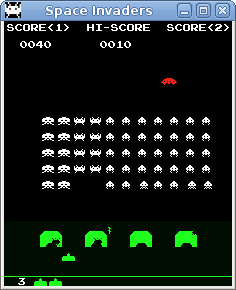
\includegraphics[scale=0.7]{space-invaders-screenshot}
  \caption{Capture d'écran du jeu \si}
  \label{Exp:si-screen}
\end{figure}

L'objectif visé en développant \si est simple: écrire un premier jeu
qui permet d'exposer les problèmes fondamentaux reliés au
développement de jeux vidéo et résoudre ces problème en tentant de
tirer profit de la puissance expressive du langage \Schemelang. Pour y
arriver, une approche de développement itératif (en spirale) a été
utilisée.

Une première version a été développée dans le but d'avoir
l'infrastructure de base du jeu et d'identifier les problèmes
rencontrés au cours du développement. Le développement de cette
première version est décrit dans la section \ref{Exp:sp1}.

Par la suite, une deuxième version fut écrite afin de répondre à
certaines lacunes que présentait la première version du jeu. Pour ce
faire, le développement du système objets présenté dans le chapitre
\ref{Chap:OO} fut entrepris. Cette démarche d'amélioration du jeu est
décrite dans la section \ref{Exp:sp2}.

Finalement, une version expérimentale fut développée. Cette version
tentait de s'éloigner de l'architecture classique de jeu vidéo où une
boucle principale (\textit{main loop}) gère l'état du système en
entier. L'idée était de tenter de fusionner le système objets et le
système de coroutine afin que tous les objets du jeu soient eux-mêmes
des coroutines, en espérant ainsi simplifier l'écriture d'entités du
jeu. En expérimentant ainsi sur le contrôle de flot du jeu, il est
possible de démontrer si l'utilisation de \Schemelang permet de faciliter
de telles expérimentations. Cette dernière version du jeu est décrite
dans la section \ref{Exp:sp3}


\FloatBarrier
\subsection{Version initiale} \label{Exp:sp1}
Dans un premier temps, l'analyse de la version arcade du jeu
disponible sur l'émulateur MAME~\cite{MAME}. Ce dernier est un système
émulant plusieurs architectures de machines arcades et permet de jouer
sur PC aux versions originales de ces jeux. Plusieurs problèmes
potentiels ont alors été identifiés:

\begin{itemize}
\item Rendu graphique du jeu
\item Flot du contrôle logique du jeu
\item Animations
\item Structures de données
\item Détection et résolution de collisions
\item Parties multi-joueurs
\end{itemize}


\FloatBarrier
\subsubsection{Rendu graphique}
Afin d'effectuer le rendu graphique du jeu, une librairie de lecture
et chargement d'images a dû être écrite. Plutôt que d'utiliser une
librairie C déjà existante pour faire ce travail, le choix de
l'écriture de cette librairie visait à limiter les dépendances
externes et d'avoir autant que possible de code en \Schemelang. Par
contre, les librairie SDL~\cite{SDL} et \textit{OpenGL}~\cite{OpenGL}
ont été utilisées afin de simplifier la gestion d'entrées/sorties, du
fenêtrage et du rendu de l'application. L'utilisation des interfaces
aux fonctions étrangères (\textit{Foreign Function Interface}) du
système Gambit-C ont fait en sorte que la tâche d'accès et
d'utilisation de ces librairies fut triviale.

Cette librairie de lecture et de chargement d'images s'occupe de lire
des images en format textuel \textit{ppm}, qui est l'un des formats
les plus simples pour décrire une image \textit{bitmap}. Le système
s'attend à lire des images sous forme de \og fontes \fg, \ie des
images contenant plusieurs sous-images. Ce choix semble raisonnable
car une entité de jeu vidéo est souvent représentée par plusieurs
images. Ceci permet donc de garder ces dernières dans une même
image. Un fichier descriptif de la fonte, sous forme de S-expressions,
doit être présent afin de permettre une interprétation correcte de la
fonte lue. Par exemple, l'image fournie dans la figure \ref{Exp:font}
doit être accompagnée d'un fichier de même nom, portant une extension
\emph{.scm} conteant la description \scheme{((colors: (white green
  red)) (chars: (0 1)))}.

\begin{figure}[htb!]
  \center
  
\includegraphics[scale=0.3]{font-example}
  \caption{Exemple de fontes utilisée dans \si.}
  \label{Exp:font}
\end{figure}

Cette fonte peut alors être lue et chargée en mémoire vidéo grâce à la
forme spéciale:

\begin{schemecode}
(define-uniform-font <font-name> <width> <height> 
                     [static] [loop-x] [loop-y])
\end{schemecode}

Cette dernière effectue la génération de code C permettant la lecture
et le chargement de la fonte spécifiée, à condition que celle-ci soit
uniforme, \ie que toutes les sous images soient de même
taille. L'option \scheme{static} permet d'effectuer la lecture durant
l'expansion macro et d'inclure l'image dans le code source généré.
Les options \scheme{loop-x} et \scheme{loop-y} permettent de spécifier
le comportement à entreprendre lorsque l'image est agrandie. Par
défaut, l'image est lue dynamiquement et est étirée lorsqu'elle est
agrandie, mais elle peut être lue dynamiquement et/ou répétée lorsque
agrandie dans la direction de l'axe des X ou des Y.

Cette librairie est très simple puisqu'elle ne traite que des fontes
aux sous-images de taille uniformes. Ce choix fut effectué puisqu'il
était bien adapté aux jeux développés et dans le but de ne pas trop
complexifier la tâche de la création des jeux.


\FloatBarrier
\subsubsection{Logique du jeu}
Le flot de contrôle de la logique de ce jeu fut expérimental dès le
départ. Dans la première version développée, une simulation par
événements discrets a été utilisée. L'idée derrière ce choix provenait
du fait que dans un jeu vidéo, la progression peut être considérée
comme une série d'événements discrets. Par exemple, le laser avance,
le joueur se déplace à droite, le vaisseau ennemi explose,
etc... Ainsi, un petit système de simulation par événements discrets a
été développé et utilisé. Ce dernier fut implanté de manière très
simple en utilisant un monceau triant les événements ordonnancés de
manière croissante en fonction du temps de leurs arrivé dans la
simulation. Ces évènements étaient des \textit{thunk}, fermetures
\Schemelang sans arguments, effectuant le travail à accomplir par
l'évènement. Lorsqu'un évènement se termine, l'ordonnanceur choisi
alors le prochain et appelle le corps de celui-ci. Il est également
possible pour un évènement d'ordonnancer un autre évènement grâce à la
forme spéciale \scheme{(in <secs> <thunk>)} qui enregistre cette
nouvelle fermeture dans le système de manière à ce qu'elle se fasse
appelée dans /scheme{<secs>} secondes. Contrairement aux simulation à
évènements discrets habituelles, les attentes du systèmes entre les
évènements sont effectuées par l'ordonnanceur de manière à respecter
les délais demandés par les évènements.

La figure \ref{Exp:des} illustre des événements qui sont ordonnancés
au tout début d'une partie. Ainsi le premier événement se chargera de
faire un \textit{dispatch} d'autres événements débutant la partie. Les
deux derniers événements sont des événements de gestion d'affichage et
d'entrées/sorties du jeu.

\begin{figure}[htb!]
  \begin{schemecode}
(schedule-event! sim 0
  (lambda () (new-player! level)
             (in 0 (create-init-invader-move-event level))
             (in 1 (create-invader-laser-event level))
             (in (mothership-random-delay)
                 (create-new-mothership-event level))))
 
(schedule-event! sim 0 (create-main-manager-event level))
(schedule-event! sim 0 (create-redraw-event level))
  \end{schemecode}
  \caption{Exemple de code de simulation par événements discrets}
  \label{Exp:des}
\end{figure}

Ces événements doivent donc s'occuper de poursuivre le calcul du jeu
leur étant assigné en réordonnant de nouveaux événements
ultérieurement dans le jeu. Par exemple, la figure \ref{Exp:mother-ev}
illustre l'évènement principal implantant le comportement désiré pour
le vaisseau mère des ennemis.

\begin{figure}[htb!]
  \begin{schemecode}
(define (create-mothership-event level)
 (define mothership-event
   (synchronized-event-thunk level
     (let ((mothership (level-mothership level)))
       (if mothership
           (let ((collision-occured? (move-object! level mothership)))
             (if (or (not collision-occured?)
                     (is-explosion? collision-occured?)
                     (eq? collision-occured? 'message))
                 (in mothership-update-interval mothership-event)))))))
  mothership-event)
  \end{schemecode}
  \caption{Évènement représentant le vaisseau ennemie de type
    \textit{mothership}.}
  \label{Exp:mother-ev}
\end{figure}

Cet exemple illustre bien deux désavantages provenant de l'utilisation
d'évènements discrets pour implanter le comportement d'entités dans un
jeu. Le premier désavantage est que la plupart des évènements sont
récursifs, et donc ils se réordonnancent par eux-mêmes un peu plus
tard dans le temps. Ceci résulte en une écriture moins intuitive de ce
comportement. Aussi, lorsqu'un évènement est déjà prévu, il est
possible que l'état du jeu change entre temps rendant cet évènement
désuet. Pour le vaisseau mère, il est possible que son prochain
déplacement ait été déjà prévu, mais que ce dernier a explosé suite à
la collision avec un laser du joueur. De tels événements sont donc
prompts à donner des erreurs dues à des inconsistances entre l'état du
jeu attendu et l'état réel lorsque se produit un événement.

Aussi, il est important de faire bien attention à doser le calcul
effectué par un événement de manière à ne pas monopoliser le temps du
processeur utilisé. Ainsi, les évènements sont souvent réordonnancés
avec un intervalle de temps de zéro, de manière à laisser la chance
aux autres évènements de s'exécuter, tout en forçant l'évènement
courant de s'exécuter le plus tôt possible.

Toutefois, cette approche semble avoir été très bénéfique pour la
création d'animations. En effet, en combinant des événements discrets
avec un style d'écriture en CPS, il est possible de bien modulariser
des animations dans le jeu. Par exemple, l'animation du début de jeu
peut être écrite sous forme CPS de manière à ce que la suite de cette
animation puisse être n'importe quel autre événement. La figure
\ref{Exp:anim} illustre une partie de l'implantation de l'animation de
début de partie. Celle-ci reçoit une continuation en paramètre. Elle
termine son animation en utilisant une animation CPS s'occupant de
faire clignoter le score du joueur. Puisqu'il s'agit de la fin de
l'animation de début de partie, la continuation est passée directement
en paramètre à cette animation de clignotement (optimisation d'appel
terminal). On a pu ainsi facilement utiliser l'animation de
clignotement, et ce de manière très modulaire, dans notre animation de
début de partie. Cette figure illustre un exemple d'utilisation de
cette animation en réécrivant de manière plus complète l'événement de
début de partie de la figure \ref{Exp:des}.

\begin{figure}[htb!]
  \begin{schemecode}
(define (start-of-game-animation-event level continuation)
  (lambda ()
    ...
    (in 0 (create-text-flash-animation-event level
            (level-get level score-msg-obj)
            animation-duration new-cont))))
(schedule-event! sim 0
  (start-of-game-animation-event level
    (generate-invaders-event level
      (lambda ()
        (new-player! level)
        (in 0 (create-init-invader-move-event level))
        (in 1 (create-invader-laser-event level))
        (in (mothership-random-delay)
            (create-new-mothership-event level))))))
  \end{schemecode}
  \caption{Exemple d'animation combinant les événements discrets et
    une programmation CPS}
  \label{Exp:anim}
\end{figure}


\FloatBarrier
\subsubsection{Structures de donnés}
Les structures de données utilisées dans \si furent définies par la
forme spéciale \scheme{define-type} de Gambit-C. Elles ont utilisé
l'héritage simple que permet cette forme de manière à tirer profit du
maximum de polymorphisme et de modularisation de code possible. La
figure \ref{Exp:deftyp-objs} donne certaines définitions des
structures employées.

\begin{figure}[htb!]
  \begin{schemecode}
(define-type game-object id type pos state color speed
  extender: define-type-of-game-object)
(define-type-of-game-object invader-ship row col)
(define-type-of-game-object player-ship)
(define-type-of-game-object message-obj text)
...
  \end{schemecode}
  \caption{Structures de données utilisées dans la première version de
    \si}
  \label{Exp:deftyp-objs}
\end{figure}

L'avantage principal de l'utilisation de ces structures est qu'elles
sont très performantes (voir la table \ref{OO:bench}). Par contre,
elles ne permettent pas d'avoir des champs communs à toutes les
instances d'un type donné. Il en résulte que l'expression du fait que
toutes les instances du type \scheme{player-ship} doivent être
associés à une boîte englobante (\textit{bounding box}) de 13 par 8
pixels est difficile à exprimer. Ces informations pourraient être
ajoutées dans chaque instances, mais ce serait un gaspillage important
d'espace mémoire puisque ces données sont communes à toutes les
instances de ce type. Ainsi, pour cette version de \textit{Space
  Invaders}, un système manuel de type \emph{très rudimentaire} a été
utilisé. Une structure de donnée décrivant un type est créée. Cette
dernière contient les données communes aux instances de ce type. Un
pointeur vers le bon type est par la suite ajouté dans le champs
\scheme{game-object-type} de chacune des instances du
jeu. L'utilisation de ce petit système de type demande ainsi une
écriture de code fastidieuse qui ne devrait pas être nécessaire.


\FloatBarrier
\subsubsection{Détection et résolution de collisions}
La détection de collisions sur ces objets a pu être faite de manière
efficace et modulaire grâce aux types qui contiennent de l'information
sur les boîtes englobantes des objets. Puisqu'il n'y a jamais beaucoup
d'objets présents dans le jeu en même temps, une détection très
rudimentaire de collisions fut utilisée. Cette dernière est présentée
dans la figure \ref{Exp:dc-si1}.

\begin{figure}[htb!]
  \begin{schemecode}
(define (detect-collision? obj level)
  (or (exists (lambda (collision-obj)
                (if (shield? collision-obj)
                    (obj-shield-collision? obj collision-obj)
                    (obj-obj-collision? obj collision-obj)))
              (level-all-objects level))
      (obj-wall-collision? obj (game-level-walls level))))
  \end{schemecode}
  \caption{Détection de collision dans \si}
  \label{Exp:dc-si1}
\end{figure}

Par contre, Un problème majeur relié à l'utilisation de ces structures
de données est apparu lorsque la \emph{résolution de collisions} a due
être implantée. En effet, cette résolution dépend du types des deux
objets entrant mutuellement en collision. La figure
\ref{Exp:si1-col-res} illustre bien le problème rencontré. On constate
que les types des objets doivent être manuellement analysés de manière
à utiliser la bonne fonction de résolution qui, elle aussi, se doit
d'analyser le type de l'objet reçu de manière a choisir la bonne
résolution à adopter. Il en résulte en du code très lourd, où il est
très facile d'introduire des erreurs.

\begin{figure}[htb!]
  \begin{schemecode}
(define (resolve-collision! level obj coll-obj)
  (cond
   ((player-ship? obj) (resolve-player-collision! level obj coll-obj))
   ((laser-obj? obj) (resolve-laser-collision! level obj coll-obj))
   ...))
(define (resolve-laser-collision! level laser-obj collision-obj)
  (cond ((invader-ship? collision-obj) ...)
        ((laser-obj? collision-obj) ...)
        ((player-ship? collision-obj) ...)
        ...))
  \end{schemecode}
  \caption{Résolution de collisions dans la première version de \si}
  \label{Exp:si1-col-res}
\end{figure}


\FloatBarrier
\subsubsection{Parties multi-joueurs}
Les parties multi-joueurs de \si sont très simples. Chaque joueur joue
en alternance jusqu'à se que son vaisseau se fasse détruire. Ainsi,
cela implique de conserver deux parties du jeu en \emph{parallèle}, où
une seule des deux avance à la fois. Avec un flot de contrôle sous
forme de simulation par événements discrets, cela implique d'avoir
deux simulations exécutées en parallèle. Puisque le système de
simulation ne permet pas d'arrêter une simulation et d'en avoir une
deuxième se produisant en même temps, une autre approche a été
utilisée. Un système de coroutines dans lequel les simulations sont
exécutées à l'intérieur de coroutines différentes a été développé et
utilisé. Ainsi, le changement de contexte peut être manuellement
utilisé lorsqu'un joueur meurt afin de réactiver la partie du prochain
joueur.

C'est de cette idée qu'est né le système de coroutine présenté dans le
chapitre \ref{Chap:corout}. Il fut initialement beaucoup plus simple
que celui présenté dans ce chapitre, mais les composantes de base
restent les mêmes. La figure \ref{Exp:si-mort} résume la procédure
utilisée lors de la mort d'un joueur. Après avoir effectué la gestion
des objets dans le niveau, un mutex est bloqué afin de permettre
l'arrêt des animations du jeu, chose requise pour l'animation de mort
d'un joueur. Ce mutex provient du système d'événement discret qui fut,
par la suite, intégré au système de coroutine. Par la suite,
l'animation de mort d'un joueur est lancée, avec comme continuation
\scheme{continuation}. Cette dernière, dans le cas où le joueur n'a
pas terminé sa partie, s'occupe d'effectuer le changement de
coroutines, après avoir informé l'autre coroutine de certaines
informations au préalable. Il est intéressant de noter que juste avant
le changement de contexte, un événement très prioritaire doit être
ordonnancé de manière à se produire immédiatement au retour du
contexte de la coroutine. Il s'agit de l'animation ré-introduisant la
partie du joueur actuel.

\begin{figure}[htb!]
  \begin{schemecode}
(define (explode-player! level player)
  (level-loose-1-life! level)
  (level-add-object! level player-expl-obj)
  (level-remove-object! level player)
  (let ((continuation
         (if (<= (game-level-lives level) 0)
             (begin ...)
             (lambda ()
               (if (2p-game-level? level)
                   (begin
                     (send-update-msg-to-other level \#f)
                     (in NOW! (start-of-game-animation-event
                               level (return-to-player-event level)))
                     (yield-corout))
                   (begin ...))))))
     (in 0 (lambda ()
            (sem-lock! (level-mutex level))
            (in 0 (player-explosion-animation-event
                   level expl-obj animation-duration continuation))))))
   \end{schemecode}
  \caption{Événement de mort d'un joueur}
  \label{Exp:si-mort}
\end{figure}


\FloatBarrier
\subsubsection{Conclusion}
Ainsi, l'écriture de cette première version de \si a permis
d'identifier plusieurs problèmes reliés au développement de jeux vidéo
(détection et résolution de collisions, parties multi-joueurs,
etc...). En plus de permettre d'expérimenter sur le type de flot de
contrôle utilisé pour développer ce jeu, \Schemelang a permis de faire
rapidement plusieurs outils non triviaux pour l'implantation du jeu,
dont un système de fontes et un petit système de coroutines.

Par contre, certains problèmes ne possèdent pas des solutions
satisfaisantes. En effet, la résolution de collision est très
fastidieuse et aurait besoin d'être modularisée et améliorée. Aussi,
la technique de flot de contrôle expérimentale utilisée (simulation
par événements discrets), fonctionne bien pour certains aspects, mais
ne semble pas naturelle pour d'autres. Ainsi, le flot de contrôle
pourrait aussi être amélioré de manière à exprimer de manière plus
naturelle le comportement des entités du jeu.


\FloatBarrier
\subsection{Version orientée objet} \label{Exp:sp2}
Une nouvelle version de \si fut développée afin de pallier à une
lacune existante dans la première version écrite: le problème relié
aux types de structures de données qui engendrait des cascades
fastidieuses de vérifications de types pour, entre autres, la
résolution de collisions (voir la figure \ref{Exp:si1-col-res}).

Initialement, plusieurs systèmes objets existant pour Gambit-C furent
mis à l'essai pour pallier à ce problème, mais aucun ne répondait bien
aux besoins présents. Certains offraient beaucoup de puissance
expressive, mais avec un coût de performance trop élevé tandis que
d'autre, plus performants, étaient trop restrictifs dans l'interface
offerte. Pour ces raisons, un système de programmation orientée objet
fut développé de manière à bien répondre aux besoins dans
\textit{Space Invaders}, sans apporter un coût d'utilisation trop
élevé. Ce système fait l'objet du chapitre \ref{Chap:OO}.

Ainsi, les objets sont maintenant déclarés comme des classes
appartenant à une hiérarchie relativement simple et tirant profit de
la possibilité de concevoir des hiérarchies multiples afin d'apposer
des propriétés aux objets du jeux. La figure \ref{Exp:sp2-class}
illustre un échantillon de la hiérarchie de classes utilisée dans le
jeu. On constate que les champs communs à toutes les instances ont été
ajoutés comme membres de classe. Une classe abstraite,
\scheme{sprite-obj}, a aussi été ajoutée afin de donner la propriété
de \textit{sprite} aux objets dont le rendu dépend d'images dans une
fonte. Par la suite, la classe \scheme{invader-ship} devient enfant de
ces deux classes, tout en ajoutant les deux champs communs à tous les
types d'\textit{invader}. Cette dernière est sous-classée par les
trois types d'ennemis existant (à l'exception du vaisseau mère qui est
traité à part). Puisque chaque type d'\textit{invader} possède sa
propre classe, on peut alors spécifier les valeurs des champs de
classes pour chacune de celles-ci de manière simple et
claire. L'utilisation de ces champs pourra être, par la suite, faite
de manière complètement uniforme et transparente. La macro
\scheme{setup-static-fields} a été écrite afin de permettre d'assigner
les champs de classes pour les classes enfants de
\scheme{game-object}.

\begin{figure}[htb!]
  \begin{schemecode}
(define-class game-object ()
  (slot: id) (slot: pos) (slot: state) (slot: color) (slot: speed)
  (class-slot: sprite-id) (class-slot: bbox)
  (class-slot: state-num) (class-slot: score-value))
(define-class sprite-obj ())
(define-class invader-ship (game-object sprite-obj) (slot: row) (slot: col))
(define-class easy-invader   (invader-ship))
(define-class medium-invader (invader-ship))
(define-class hard-invader   (invader-ship))
(setup-static-fields! easy-invader 'easy (make-rect 0 0 12 8) 2 10)
(setup-static-fields! medium-invader 'medium (make-rect 0 0 12 8) 2 20)
(setup-static-fields! hard-invader 'hard (make-rect 0 0 12 8) 2 30)
  \end{schemecode}
  \caption{Aperçu de la hiérarchie de classe du jeu}
  \label{Exp:sp2-class}
\end{figure}

L'attrait principal du développement et de l'intégration du système
objet pour la création du jeu réside dans l'utilisation des fonctions
génériques. L'utilisation de celles-ci permet d'utiliser des
opérations spécifiques aux objets de manière complètement
transparente, rendant ainsi l'écriture de ces parties du code plus
élégante et solides face aux changements éventuels des structures de
donnés ou de l'architecture du jeu.

Trois fonctions génériques ont été utilisées pour améliorer \si:
\scheme{detect-collision?}, \scheme{resolve-collision!} et
\scheme{render} qui effectuent respectivement la détection de
collisions, la résolution de collisions et le rendu graphique des
objets. La figure \ref{Exp:si2-genfun} donne un aperçu de
l'utilisation faite de la fonction générique
\scheme{resolve-collision!}. Des instances de cette dernière sont
définies pour les paires de collisions possibles dans le jeu et le
système s'occupe de faire automatiquement le choix dynamique de la
bonne instance en fonction des objets passés en paramètre. Le code
résultant est beaucoup plus modulaire et clair que celui de la version
précédente du jeu.

\begin{figure}[htb!]
  \begin{schemecode}
(define-method (resolve-collision! level (laser laser-obj) (inv invader-ship))
  (invader-ship? inv) 
  (level-increase-score! level inv)
  (destroy-laser! level laser)
  (explode-invader! level inv))

(define-method (resolve-collision! level (laser1 laser-obj) (laser2 laser-obj))
  (let ((inv-laser (if (player\_laser? laser1) laser2 laser1)))
    (explode-laser! level inv-laser)
    (destroy-laser! level inv-laser)))
...
(define (move-object! level obj)
  (move-object-raw! obj)
  (let ((collision-obj (detect-collision? obj level)))
    (if collision-obj
        (begin (resolve-collision! level obj collision-obj)
               collision-obj)
        \#f)))
  \end{schemecode}
  \caption{Exemple de définition et d'utilisation d'une fonction
    générique dans \si}
  \label{Exp:si2-genfun}
\end{figure}

La deuxième version du jeu apporte beaucoup d'améliorations face au
développement de jeu vidéo en \Schemelang grâce à l'utilisation de la
programmation orientée objet. La modularité et l'abstraction du code
de la première version a été améliorée de grâce à l'utilisation d'une
hiérarchie de classes annotée de propriétés et comportant des membres
de classe et des fonctions génériques pour effectuer de manière
transparente les actions de base sur les instances de ces classes. Par
contre, un problème n'a toujours pas été adressé dans cette nouvelle
version. En effet, le flot de contrôle implanté par une simulation à
événement discret n'a pas été modifié afin de mieux l'adapter aux
comportements des entités du jeu.


\FloatBarrier
\subsection{Version avec flot de contrôle sous forme de coroutines} \label{Exp:sp3}
Ainsi, après deux version du jeu, \si possède toujours certains
problèmes dont le flot de contrôle utilisé qui n'est très bien adapté
aux objets du jeu. Afin d'adresser ce problème, le système de
coroutines utilisé pour l'implatation de parties multi-joueurs a été
étendu de manière à ce que le flot de contrôle des entités du jeu soit
exprimé plutôt sous forme de \emph{coroutines}. Ce système est
présenté dans le chapitre \ref{Chap:corout}. Cette approche sur le
contrôle de flot est aussi expérimentale, mais l'utilisation d'une
simulation à événements discrets a laissée croire que la description
du comportent des entités sous forme de \textit{threads} serait plus
naturelle. En effet, en utilisant des événements discrets, le corps
des événements devait faire en sorte que l'événement se poursuive en
se réordonnançant un peu plus tard, donnant ainsi la chance aux autres
événements de s'exécuter. Ce phénomène correspond très bien à la
fonction \scheme{yield} du système de coroutine qui interrompt de
manière temporaire l'exécution d'une coroutine afin de laisser la
chance aux autres coroutines de continuer leur travail.

Ainsi, dans cette nouvelle version du jeu, \emph{tous} les objets sont
maintenant des coroutines exécutant leurs comportement de manière
indépendante. Pour ce, une version orientée objet du système de
coroutine fut produite. La figure \ref{Exp:si3-class} illustre
l'intégration du système de coroutine aux objets du jeu. L'utilisation
de constructeurs permet l'appel du constructeur de base des coroutines
afin de spécifier le comportement que devra entreprendre l'objet. Ce
corps est déterminé de manière dynamique avec la fonction générique
\scheme{behaviour} et sera exécuté dans un environnement contenant des
gestionnaires de messages dynamiques, communs à tous les objets,
permettant de pauser le jeu ou de détruire ces derniers.

\begin{figure}[htb!]
  \begin{schemecode}
(define-class game-object (corout)
  (slot: pos)
  (slot: state)
  (slot: color)
  (slot: speed)
  (class-slot: sprite-id)
  (class-slot: bbox)
  (class-slot: state-num)
  (class-slot: score-value)
  (constructor: (lambda (obj id pos state color speed level)
                  (init! cast: '(corout * *) obj id
                         (lambda ()(with-dynamic-handlers
                                    ((pause (pause obj level))
                                     (die   (die   obj level)))
                                    ((behaviour obj level)))))
                  (set-fields! obj game-object
                    ((pos pos)     (state state)
                     (color color) (speed speed))))))
  \end{schemecode}
  \caption{Classe de base des objets en tant que coroutine}
  \label{Exp:si3-class}
\end{figure}

Malgré l'idéologie prometteuse d'avoir des objets indépendant régis
chacun par leurs propres comportements, l'implantation du comportement
des entités du jeu est devenu très rapidement
\emph{cauchemardesque}. En effet, puisque toutes les entités possèdent
leurs fils d'exécution et que ceux-ci sont tous équivalents, la
\emph{synchronisation} entre ces dernière est primordiale et implique
des protocoles de communication complexes entre les objets. Ces
protocoles doivent régir tout le comportent du jeu et, en bout de
ligne, le flot de contrôle devient soudainement très difficile à
exprimer. Ainsi, des méta-objets ont dû être introduits afin
d'effectuer la synchronisation entre les objets de base, comme les
ennemis. La figure \ref{Exp:inv-cnt} donne le comportement du
méta-objet régissant l'activité d'une rangée d'\textit{invader}. Ce
dernier utilise des listes de diffusions pour envoyer des messages aux
\textit{invader} de la rangée qu'il coordonne. Il possède deux états:
l'état initial qui attend la réception d'un message lui indiquant que
c'est le tour de sa rangée de se déplacer et un deuxième état
consistant à une barrière de synchronisation effectuant l'attente de
la réception du message \scheme{moved} de la part de tous les
\textit{invader} de la rangée. Puis, il vérifie si une collision s'est
produite avec un mur durant se déplacement et effectue la gestion de
cette collision si c'est le cas en avertissant les autres contrôleurs
de la situation.

De plus, l'utilisation intensive (voir abusive) du système de
coroutine couplé avec le système d'objets a résulté en une chute
dramatique des performances du jeu. Cette chute de performance a
permis d'améliorer le système de coroutine en implantant un système de
profilage des coroutine afin de visualiser quelles coroutines
monopolisaient le contrôle de l'ordonnanceur pour une durée trop
longue. Il était ainsi possible d'optimiser certaines coroutines afin
d'améliorer les performances globales du système. Toutefois, même
après effectuer ces optimisations, les performances du jeu demeuraient
très mauvaises et donc, la troisième itération de \si fut abandonné en
cours de route. La majeur partie de la logique du jeu fut implanté
sous forme de coroutines. Cette version a permis de réaliser que
l'approche plus tradionnelle pour le flot de contrôle serait plus
appropriée que les approches utilisées pour implanter \si. Par contre,
cette expérimentation sur la technique de flot de contrôle a permis de
démontrer la facilité avec laquelle il a été possible de modifier le
coeur du jeu pour essayer de nouvelles options quant à l'architecture
du programme et de son flot de contrôle.

\begin{figure}[htb!]
  \begin{schemecode}
(define (invader-controller)
  (define (init-state)
    (recv
     (init
      (subscribe instant-components (self))
      (broadcast `(invader-row ,(Inv-Controller-row (self)))
                 'move)
      (wait-state))))
  (define-wait-state wait-state moved (inv-nb)
    (recv
     (go-down-warning
      (let ((row-nb (Inv-Controller-row (self))))
        (broadcast `(invader-row ,row-nb) 'wall-collision)
        (for i 0 (< i invader-row-number)
             (if (not (= i row-nb))
                 (if (not (zero? (msg-list-size `(invader-row ,i))))
                     (let ((move-back? (< i row-nb)))
                       (broadcast `(invader-row ,i)
                                  `(wall-collision ,move-back? \#f))))
                 (broadcast `(invader-row ,i)
                            `(wall-collision  \#t ,(self))))))
      (wait-state))
     (after 0
            (wait-for-next-instant)
            (broadcast `(row-controller
                         ,(next-row (Inv-Controller-row (self))))
                       'init)
            (unsubscribe instant-components (self))
            (init-state))))
  (init-state))
  \end{schemecode}
  \caption{Comportement du méta-objet \scheme{invader-controller} qui
    régi le comportement d'une rangée d'\textit{invaders}}
  \label{Exp:inv-cnt}
\end{figure}


\FloatBarrier
\subsection{Conclusion}
Ainsi, le développement de \si en \Schemelang fut très riche en
expériences. Il a permis de trouver plusieurs problèmes reliés au
développement de jeux vidéo. Ces derniers ont été résolus en utilisant
le mieux possible les avantages qu'offrent un langage de haut niveau
tel que \Schemelang en utilisant les fonctions d'ordres supérieures, un
style de programmation CPS et en développant un système de coroutines.

La création d'un système de programmation orienté objet a grandement
permis d'améliorer la qualité du code écrit lors du développement de
la première version du jeu grâce à l'utilisation des fonctions
génériques permettant de faire un choix dynamique de procédures en
fonctions des objets passés en paramètres. Notamment, la résolution de
collision , qui dépend du types des deux objets en question, a pu être
écrite de manière très élégante et modulaire grâce aux fonction
génériques.

L'expérimentation effectuée sur le flot de contrôle du jeu a permis de
démontrer que l'architecture du moteur peut être modifiée afin de
mettre à l'essai de nouvelles techniques de gestion du flot de
contrôle pour jeu. L'utilisation du système de coroutines permis
d'implanter efficacement une version multi-joueurs du jeu, mais fut
inappropriée pour effectuer la gestion complète du flot de contrôle du
jeu.

Puisque \si est un jeu très simple, la gestion mémoire automatique n'a
jamais constituée un obstacle au développement puisque trop peu
d'objets étaient utilisés et les pauses dues à la récupération mémoire
utilisaient environ 2 millisecondes, soit environ 1\% du temps
processeur requis pour le rendu d'une image.

Il serait maintenant intéressant d'implanter un jeu plus complexe afin
de valider si les techniques utilisées pour \si sont toujours
applicables et de voir si elles s'étendent bien aux nouveaux défis de
programmations résultant de l'implantation d'un tel jeu.


\FloatBarrier
\section{Développement de \lr} \label{Exp:ld}
Après avoir développé \textit{Space Invaders}, un deuxième jeu a dû
être développé afin de consolider les techniques
développées. Le jeu \lr a été choisi dans le but de remplir cette
tâche pour plusieurs raisons. Principalement, ce jeu contient de
nouveaux éléments qui n'étaient pas présent dans \si comme le concept
d'intelligence artificielle et étendait d'autre concepts qui y étaient
très primitifs comme le concept de niveaux et d'états d'entités.

Ce jeu consiste à tenter de capturer tout l'or dispersé dans le niveau
en évitant de rentrer en contact avec les robots ennemis. Pour y
arriver, le joueur doit grimper des échelles, passer sur des cordes et
utiliser son pistolet laser qui permet de faire des trous à la gauche
ou à la droite du joueur. Ces trous se referment après un délais
prescrits et donc les joueurs doivent se dépêcher afin d'éviter de
rester pris au piège à l'intérieur d'un trou. Lorsque tout l'or est en
possession du joueur, une échelle de sortie apparaît et mène le joueur
au niveau suivant. La joueur dispose de trois vies pour se rendre le
plus loin possible dans le jeu et obtenir le meilleur score
possible. La figure \ref{Exp:ld-screen} illustre une capture d'écran
du jeu développé.

\begin{figure}[htb!]
  \center
  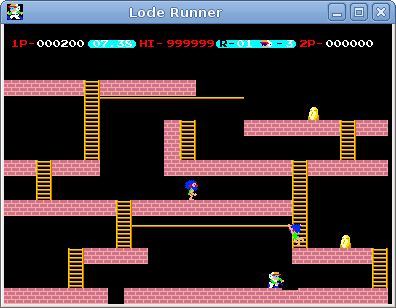
\includegraphics[scale=0.6]{lode-runner-screenshot}
  \caption{Capture d'écran du jeu \lr développé}
  \label{Exp:ld-screen}
\end{figure}


\FloatBarrier
\subsection{Logique du jeu}
Afin de développer ce jeu, les meilleurs techniques utilisées pour le
développement de \si ont été réutilisées et raffinées pour les besoins
plus grands de \lr. Par contre, le flot de contrôle de la logique du
jeu est régi de manière beaucoup plus conservatrice en utilisant une
boucle principale effectuant le travail à faire pour chaque image du
jeu (\textit{Game Loop}). Il en résulte qu'une fonction générique
\scheme{animate} est appelée avant le rendu de chaque image de manière
à effectuer le travail que doit accomplir chaque objet avant ce
rendu. La figure \ref{Exp:lr-main} illustre une partie de la boucle
principale du jeu et l'instance de la fonction générique
\scheme{advance-frame!} pour un niveau de jeu. Cette figure illustre
la simplicité du flot de contrôle du jeu résultante grâce à
l'utilisation de fonction génériques et de fonctions d'ordre
supérieures.

\begin{figure}[htb!]
  \begin{schemecode}
(define-method (advance-frame! (level level) keys-down keys-up)
  (cond ((level-get 'player level) =>
         (lambda (player)
           (player-velocity-set! player point-zero))))
  (cond
   ((level-paused? level) 'do-nothing)
   ...
   (else
    (update! level level current-time (lambda (t) (+ t (fl/ 1. (FPS)))))
    (if (> (level-current-time level) (level-time-limit level))
        (level-game-over! level)
        (begin
          (for-each (flip process-key level) keys-down)
          (for-each (flip animate level) (level-objects level)))))))

;; Game loop
(let loop ((level (current-level)))
  (if exit-requested? (quit))
  (poll-SDL-events)
  (advance-frame! level (key-down-table-keys) (key-up-table-keys))
  (render-scene screen level)
  (loop (current-level)))
  \end{schemecode}
  \caption{Boucle principale du jeu \lr}
  \label{Exp:lr-main}
\end{figure}

Par contre, l'utilisation d'une telle boucle fait en sorte que la
vitesse du jeu dépend directement du taux de rafraîchissement de
celui-ci.


\FloatBarrier
\subsection{Gestion de l'état des objets}
Les entités du jeu \lr sont sensiblement plus complexes que celles
présente dans le jeu précédant. En effet, ces dernières possèdent sont
animés et réagissent différemment en fonction du contexte de
celle-ci. Encore une fois, ce sujet est traité de manière
traditionnelle en utilisant des états d'objets et des machines à états
afin de régir leurs comportements et les animations de ceux-ci. La
figure \ref{Exp:hl} donne le contenu de la classe \scheme{human-like}
qui sert de base aux classes \scheme{player} et \scheme{robot} qui
implantent respectivement les instances du joueurs et des robots
ennemis. Elle démontre bien la complexité de l'état de ces entités.

\begin{figure}[htb!]
  \begin{schemecode}
(define-class human-like (game-object moving statefull)
  (slot: can-climb-up?)
  (slot: can-go-down?)
  (slot: can-use-rope?)
  (slot: can-walk?)
  (slot: droped-rope?)
  (slot: stuck-in-hole?)
  (slot: facing-direction)
  (slot: walk-cycle-state)
  (slot: shooting?)
  (slot: escaping?)
  (constructor: (lambda (self x0 y0 initial-velocity id) ...)))
  \end{schemecode}
  \caption{Définition de la classe \scheme{human-like} dans le jeu \lr}
  \label{Exp:hl}
\end{figure}

La fonction générique \scheme{change-state!}  utilise l'état des
instances de ces classes pour déterminer l'animation qui doit être
utilisée afin d'obtenir un rendu cohérent de l'entité. La figure
\ref{Exp:lr-change-state} contient la gestion principale de l'état des
entités appartenant à la hiérarchie de la classe
\scheme{human-like}. Ici, avant le rendu de chaque image, l'état de
chaque objet est vérifié et mis-à-jour. Puisque les états possibles
d'une instance de la class \scheme{human-like} ne sont pas
orthogonaux, \ie que plusieurs états correspondant à des animations
différentes peuvent être présent en même temps, l'ordre de la
modification de l'état est significative. Si ces derniers avaient été
orthogonaux, la gestion de ceux-ci aurait pu être effectuée en
utilisant la discrimination de méthodes sur les valeurs de ces
états. Le code résultant aurait donc été très limpide.

\begin{figure}[htb!]
  \begin{schemecode}
(define-method (change-state! (hl human-like) level)
  (let* ((v (moving-velocity hl)))
    (cond
     ((eq? (human-like-escaping? hl) 'escaping) (ascend-cycle! hl))
     ((human-like-shooting? hl)                 (shoot-cycle hl))
     ((human-like-stuck-in-hole? hl)            (dying-cycle! hl))
     ((and (not (zero? (point-x v))) 
           (human-like-can-walk? hl))
                                                (walk-cycle! hl))
     ((human-like-can-use-rope? hl)
       (if (or (not (zero? (point-x v)))
               (not (memq (human-like-state hl) rope-states)))
           (rope-cycle! hl)
           'keep-same-state^\_^))
     ((not (human-like-can-go-forward? hl))     (fall-cycle! hl))
     ((not (zero? (point-y v)))                 (ascend-cycle! hl))
     (else (reset-walk-cycle! hl)))))
  \end{schemecode}
  \caption{Gestion de l'état d'une entité appartenant à la hiérarchie
    de type \scheme{human-like} dans \lr}
  \label{Exp:lr-change-state}
\end{figure}

Les fonctions d'animation des entités (\scheme{walk-cycle},
\scheme{rope-cycle!}, ...) produisent des animations se répétant de
manière cyclique. Puisque ce genre d'animation est fréquente dans le
jeu, elle fut abstraite dans une forme spéciale afin de simplifier la
définition de celles-ci. La figure \ref{Exp:cyclic-anim-dsl} présente
cette dernière qui construit une définition de fonction qui met-à-jour
les champs \scheme{cycle-member} et \scheme{state-member} afin de
produire correctement le rendu de l'animation. Le champs
\scheme{cycle-member} de l'instance reçue contiendra un nombre
correspondant à l'état actuel de l'animation. Cet état est conservé
dans l'attribut \scheme{state-member} et sera utilisé par l'algorithme
de rendu graphique du jeu. Le paramètre \scheme{cycle-delta}
représente le nombre d'images qui seront rendues avant le changement
de l'état actuel de l'entité.

\begin{figure}[htb!]
  \begin{schemecode}
(define-macro (define-cyclic-animation name
                \#!key base-class cycle-delta cycle-member
                      state-member states other-actions-fun)
  (let ((obj (gensym 'obj))
        (cycling-delta (gensym 'cycling-delta))
        ...)
    `(define (,name ,obj)
       (let* ((,cycle-length (* ,cycle-delta ,(length states))))
         (update! ,obj ,base-class ,cycle-member
                  (lambda (s) (modulo (+ s 1) ,cycle-length)))
         (let ((,next-state
                (case (quotient (,cycle-member-getter ,obj) ,cycle-delta)
                  ,@(map-with-index (lambda (i x) `((,i) ',x)) states)
                  (else (error ...)))))
           (,state-member-setter ,obj ,next-state)
           (,other-actions-fun ,obj))))))
  \end{schemecode}
  \caption{Forme spéciale utilisée afin de simplifier la définition
    d'animations cycliques d'entité du jeu \lr}
  \label{Exp:cyclic-anim-dsl}
\end{figure}

Ainsi les animations du jeu peuvent être définies en utilisant cette
forme spéciale. La figure \ref{Exp:cyclic-anim-def} illustre la
définition de l'animation de marche utilisée par les sous-classes de
la classe \scheme{human-like}. On peut donc ainsi tirer profit du
polymorphisme du système objets en plus du petit langage de définition
d'animations afin de définir de manière claire et concise une
animation cyclique.

\begin{figure}[htb!]
  \begin{schemecode}
(define-cyclic-animation walk-cycle!
  base-class: human-like
  cycle-delta: 5
  cycle-member: walk-cycle-state state-member: state
  states: (standing-up standing-left standing-up standing-right)
  other-actions-fun:
    (lambda (obj) (human-like-facing-direction-set!
                   obj (human-like-get-direction obj))))
  \end{schemecode}
  \caption{Définition d'animation cyclique dans le jeu \lr}
  \label{Exp:cyclic-anim-def}
\end{figure}

En plus de considérer les objets du jeu comme des machines à états,
les niveaux eux-mêmes peuvent aussi être considérés comme tel. En
effet, on peut subdiviser le flot d'un niveau en 6 états différents:
\scheme{pre-game}, \scheme{start}, \scheme{in-game}, \scheme{paused},
\scheme{game-over} et \scheme{level-cleared}.  La figure
\ref{Exp:lr-state-diag} illustre les transitions possibles entre ces
derniers. Chaque états sont justifiés par un comportement différent du
niveau, soit par une gestion différente des entrées du joueurs comme
c'est le cas pour l'état \scheme{paused} ou encore par un rendu
graphique différent du niveau.

\begin{figure}[htb!]
  \center
  \includegraphics[scale=0.7]{lr-state-diag}
  \caption{Diagramme d'états d'un niveau de \lr}
  \label{Exp:lr-state-diag}
\end{figure}

Afin d'implémenter ce système de machines à états, un petit langage
spécifique au domaine a été développé. Ce dernier tire avantage du
système de programmation orienté objet utilisé, notamment de la
discrimination de méthodes sur des valeurs afin de valider les
transitions effectuées. Sans trop entrer dans les détails, il ne
suffit que de sous-classer la classe \scheme{state-machine} par les
objets de niveaux et d'ensuite effectuer la déclaration qui se fait
selon l'interface présentée dans la figure \ref{Exp:def-state}. Les
états sont normalement décrits par des symboles. Les actions peuvent
être n'importe quelles expression \Schemelang. Aussi, lors de la
description des transitions, il est possible d'utiliser le symbole
\scheme{*} afin de représenter tous les états possibles ou sinon
d'utiliser une sous-liste contenant les états de provenance ou
d'arrivé pour cette transition. La figure
\ref{Exp:lr-lvl-state-machine}.

\begin{figure}[htb1]
  \begin{schemecode}
(define-state-machine <class-name> <init-state> <init-action> <state-list>
                      ((<from-state> <to-state> <transition-action>) ...))
  \end{schemecode}
  \caption{Interface du système de machines à états développé pour les
    niveaux de \lr}
  \label{Exp:def-state}
\end{figure}

\begin{figure}[htb!]
  \begin{schemecode}
(define-class level (menu state-machine) ...)

(define-state-machine level
  'pre-game pre-game-transition
  (pre-game start in-game game-over level-cleared paused)
  ((pre-game start         level-start-transition)
   (start    in-game       level-in-game-transition)
   (in-game  game-over     level-game-over-transition)
   (in-game  level-cleared level-cleared-transition)
   (in-game  paused        level-paused-transition)
   (paused   in-game       level-paused-transition)
   (* * (lambda (self) (println "unknown transtion into " to))))
  create-new-class?: \#f)
  \end{schemecode}
  \caption{Implantation de la machine à états pour les niveaux dans \lr}
  \label{Exp:lr-lvl-state-machine}
\end{figure}

Les actions utilisées lors des transitions servent principalement à
initialiser le nouvel état du niveau. Les fonctions de rendu et de
gestion des entrées du joueur s'occupent elles-mêmes de faire la
distinction entre ces états. Par exemple, la fonction
\scheme{level-start-transition} qui sert à faire le compte à rebours
du début de la partie s'occupe d'ajouter un nouvel objet représentant
une chaîne de caractères qui contient le compte à rebours. Ce dernier
utilise la récursivité afin de se recréé avec le rebours mis-à-jour à
tous les 60 images rendues.

\begin{figure}[htb!]
  \begin{schemecode}
(define (level-start-transition lvl)
  (define (make-counter-label counter)
    (if (>= counter 0)
        (let ((lab
               (new label
                    'start-counter
                    (if (zero? counter) "Start!" (number->string counter))
                    24 18 'green
                    (list (lifetime 60
                                    (lambda (l lvl)
                                      (level-delete! l lvl)
                                      (make-counter-label (- counter 1))))))))
          (gui-centered?-set! lab \#t)
          (gui-scale-ratio-set! lab 4.)
          (level-add! lab lvl))
        (transition lvl 'in-game)))
  (make-counter-label 3))
  \end{schemecode}
  \caption{Action de transition vers l'état \scheme{start} d'un niveau
    du jeu \lr}
  \label{Exp:lr-start-transition}
\end{figure}

Ainsi, les macros et les fonctions d'ordre supérieures de \Schemelang
ont permis d'exprimer de manière élégante et modulaire les concepts
reliés à la déclarations de machines à états pour les entités ainsi
que les niveau du jeu \textit{Lode Runner}.


\FloatBarrier
\subsection{Détection et résolution de collisions}
Une nette amélioration apportée au jeu, en comparaison celui
développé précédemment, est l'utilisation d'une grille pour accélérer
la détection de collisions. Le principe est simple: une grille
bidimensionnelle contenant un nombre de subdivisions variable est
créée. Lorsqu'un objet est ajouté au jeu, il est ajouté dans chacune
des cases de la grilles auxquelles il entre en contacte et,
réciproquement, cet objet possède des pointeurs vers chacune de ces
cases de la grille. Si la grille est assez fine, alors la détection de
collisions devient triviale: il ne suffit que de regarder dans cases
de la grille qui touchent l'objet en question afin de voir si d'autres
objets s'y trouvent et si c'est le cas, alors une collision est
détectée. Bien sûr, la taille de la grille influence sur le travail
nécessaire lors de chaque ajout et déplacement d'objets, mais puisque
dans \lr la plupart des objets sont statiques, cela ne pose pas de
problèmes réels. La figure \ref{Exp:lr-col-detection} illustre
l'algorithme de détection de collisions utilisé.

\begin{figure}[htb!]
  \begin{schemecode}
(define (detect-collisions obj level)
  (filter (lambda (x) (not (eq? x obj)))
          (fold-l (curry2* set-union eq?)
                  '()
                  (map (curry2 grid-get (level-grid level))
                       (game-object-grid-cells obj)))))
  \end{schemecode}
  \caption{Détection de collisions dans \lr}
  \label{Exp:lr-col-detection}
\end{figure}

La résolution de collisions ainsi que le rendu graphique sont
effectués tous deux de manière très similaire à ce qui a été utilisé
dans \si. Des fonctions génériques \scheme{resolve-collision} et
\scheme{render} s'occupent de choisir dynamiquement la bonne instance
de ces fonctions génériques en fonction des objets passés. 


\FloatBarrier
\subsection{Rendu graphique}
Il est intéressant de noter que le rendu graphique est légèrement plus
complexe que pour le jeu \si, car il est possible d'avoir des objets
qui se superposent. Afin de résoudre les problèmes de visibilités qui
en résultent, l'algorithme du peintre a été utilisé. Ce dernier est
implanté en utilisant des couches sur lesquelles doivent apparaître
les objets afin de donner des priorités de rendu. Comme l'indique la
figure \ref{Exp:layers}, le joueur se trouve sur la couche
\scheme{human-like-layer} qui est prioritaire aux couches des objets
du jeu, résultant en l'affichage du joueur par dessus ces
derniers. Les objets sont triés lorsque des nouveaux objets sont
ajoutés au niveau afin d'éviter à faire ce tri lors du rendu de chaque
images.

\begin{figure}[htb!]
  \begin{schemecode}
(enum background-layer stage-layer foreground-layer human-like-layer top-layer)
(define-method (get-layer (h human-like))    human-like-layer)
(define-method (get-layer (h hole))          foreground-layer)
(define-method (get-layer (s stage))         stage-layer)
(define-method (get-layer (obj game-object)) foreground-layer)
  \end{schemecode}
  \caption{Implantation des couches de rendu dans \lr}
  \label{Exp:layers}
\end{figure}


\FloatBarrier
\subsection{Intelligence Artificielle}
L'intelligence artificielle du jeu fut implantée de manière directe en
utilisant des fermeture afin d'abstraire les différents algorithmes
potentiels (proposant différentes difficultés au joueurs). Seuls deux
algorithmes furent toutefois implantés pour le jeu. Le premier,
complètement trivial, fait en sorte que les robots demeurent
immobiles.  Le deuxième utilise un environnement totalement observable
et reproduit un comportement \emph{similaire} à celui des ennemis de
la version originale. Ces algorithmes sont présentés dans les figures
\ref{Exp:ai-imm} et \ref{Exp:ai-seek}. Les fermetures contenant ces
algorithmes sont utilisées de manière dynamique en fonction du niveau
de difficulté choisi par le joueur. Il est ainsi possible de modifier
durant la partie la difficulté. Aussi, l'utilisation de fermeture
donne la chance de créer de nouvelles fermetures contenant des
informations plus spécialisées pour l'état actuel du
jeu. L'implantation du choix dynamique de l'algorithme d'intelligence
artificielle est présenté dans la figure \ref{Exp:dyn-ai}.

\begin{figure}[htb!]
  \begin{schemecode}
(define (immobile-ai robot level)
  (robot-velocity-set! robot point-zero))
  \end{schemecode}
  \caption{Algorithme trivial d'intelligence artificielle des robots}
  \label{Exp:ai-imm}
\end{figure}

\begin{figure}[htb!]
  \begin{schemecode}
(define (seeker-ai robot level)
  (let ((player (level-get 'player level)))
    (if player
        (let* ((dir (point-sub player robot))
               (y-axis? (let ((x (point-x dir)) (y (point-y dir)))
                          (and (not (zero? y))
                               (can-go-up/down? robot x y))))
               (velo (if y-axis?
                         (new point 0 robot-movement-speed)
                         (new point robot-movement-speed 0)))
               (factor (if (< (if y-axis? (point-y dir) (point-x dir)) 0)
                           -1
                           1)))
          (robot-velocity-set! robot (point-scalar-mult velo factor))))))
  \end{schemecode}
  \caption{Algorithme d'intelligence artificiel reproduisant un
    comportement \emph{similaire} au jeu original}
  \label{Exp:ai-seek}
\end{figure}

\begin{figure}[htb!]
  \begin{schemecode}
(define (get-ai-fun difficulty)
  (case difficulty
    ((easy) immobile-ai)
    ((hard) seeker-ai)
    (else immobile-ai)))

(define (run-ai robot level)
  ((get-ai-fun (level-difficulty level)) robot level))
  \end{schemecode}
  \caption{Utilisation dynamique des algorithmes d'intelligence
    artificielle}
  \label{Exp:dyn-ai}
\end{figure}


\FloatBarrier
\subsection{Conclusion}
L'implantation du jeu \lr a permis de consolider certaines des
techniques d'implantation de jeux développés pour \si. En effet,
l'utilisation de fonctions génériques a permis d'exprimer simplement
et de manière très \emph{modulaire} le comportement des objets dans le
jeu.

Le flot de contrôle du jeu a été implanté de manière beaucoup plus
traditionnelle que ce fut le cas pour \si. Il en résulte que le jeu
dépend beaucoup des notions d'états des objets. Puisque le langage
\Schemelang offre le meilleur des deux mondes, \ie qu'il offre un langage
fonctionnel permettant des mutations, ce type de contrôle de flot a
permis de tirer profit des avantages qu'offrent la programmation
fonctionnelle (fonctions d'ordre supérieures, fermetures, etc...) tout
en utilisant un modèle éprouvé de flot de contrôle et de
modularisation.

La gestion des états plus complexes des objets du jeu a pu être écrite
de manière très élégante grâce à la conception d'un langage spécifique
au domaine minimaliste. Il fut ainsi possible de décrire le \og quoi
\fg des animations tout en cachant la mécanique commune aux animations
des entités du jeu.

L'ajout d'une grille pour accélérer la détection de collisions semble
peut-être peu significative puisque \lr ne contient pas une très
grande quantité d'objet, mais ce système a été ajouté dans le but de
facilement et rapidement implanter des jeux qui seront plus complexes
et qui nécessiteraient de tels optimisations.

Tout comme ce fut le cas pour \si, la gestion mémoire automatique n'a
pas été un problème pour le développement de ce jeu. En effet, malgré
un plus grand nombre d'objets présents, ceux-ci demeurent trop peu
pour éprouver la gestion mémoire sur des ordinateurs récents.


\FloatBarrier
\section{Conclusion}
Ainsi, il a été possible de développer deux jeux vidéo de complexité
croissante en utilisant le langage \Schemelang. Le développement du premier
jeu, \si, a permis d'identifier et de répondre aux besoins
fondamentaux de jeux vidéo: rendu graphique, détection de collisions,
etc... Pour ce faire, un système de programmation orienté objet et un
système de coroutines ont été ajouté au langage \Schemelang. Aussi, le
premier jeu a permis de vérifier la difficulté inhérente au changement
de l'architecture du flot de contrôle d'un jeu en passant d'un flot
contrôlé par une simulation par événements discrets à une simulation
par agents. La conversion s'est faite sans trop d'efforts, grâce aux
abstractions utilisées dans le jeu.

Un deuxième jeu a, par la suite, été développé afin de permettre de
vérifier si les techniques utilisées pour \si s'adaptaient à un autre
jeu plus complexe. Ainsi, \lr fut développé en utilisant les
abstractions de haut niveau que permettent les fonctions de première
classe combinées avec un système d'objets très polyvalent et la
conception de nouvelles formes spéciales. En utilisant, cette fois ci,
une approche conservatrice sur le flot de contrôle. Le résultat fut
très clair: le jeu a été développé rapidement et sans problèmes
importants.

Ainsi, il serait maintenant intéressant de voir quel serait l'impact
de l'implantation en \Schemelang d'un jeu de qualité commerciale afin de
tester plus profondément les limites que pourrait imposer le langage
sur des jeux plus exigeant tant en utilisation processeur qu'en
utilisation mémoire.





\clearpage

%%%%%%%%%%%%%%%%%%%%%%%%%%%%%%%%%%%%%%%%%%%%%%%%%%%%%%%%%%%%%%%%%%%%%%%%%%%%%%%
\chapter{Travaux reliés}
Les langages de programmation de la famille \lisp ont déjà été
utilisés pour produire des jeux vidéo commerciaux de très bonne
qualité. Certains seront cités et une revue de l'expérience acquise
par les développeurs sera exposée dans le but de comparer leurs
expériences avec celle acquise pour le développement de \si et de \lr.

Avant tout, nous comparerons les différents langages utilisés dans
l'industrie du jeu vidéo avec \Schemelang afin d'en faire ressortir les
forces et faiblesses. Les différences mènent à des méthodes de
développement qui seront nécessairement divergentes. Ainsi, un
portrait des techniques de programmation utilisées dans l'industrie
est dressé dans le but de bien situer les travaux présentés dans ce
mémoire.


\FloatBarrier
\section{Comparaison de langages}
L'industrie du jeu vidéo est déjà bien établie et donc, certains
langages sont favorisés quant au développement de jeux vidéo par les
compagnies oeuvrant dans le domaine. Cette section présente ces
langages dans le but de les comparer à \Schemelang afin de mettre en
lumière la possibilité de les remplacer par ce dernier.

Les critères de comparaison utilisés dans cette section comprennent
les fonctionnalités offertes par ces langages, le typage utilisé dans
ceux-ci, le niveau d'abstraction du langage ainsi que les modes
d'utilisations de celui-ci. 


\FloatBarrier
\subsection{C++}
Le langage principalement utilisé pour le développement de jeu vidéo
est sans aucun doute le langage C++~\cite{cplusplus}. Ce dernier est
une version orientée objet du langage C qui est aussi très répandu et
apprécié pour être un langage suffisamment de bas niveau pour
permettre d'écrire du code très efficace. Ainsi, C++ apporte les
paradigmes de la programmation orientée objet en introduisant des
classes à héritage multiple et des fonctions virtuelles permettant un
\textit{dispatch} dynamique simple. C++ possède également un système
de gestion d'exceptions et de \textit{templates}.

Ainsi, le langage C++ semble être grandement apprécié pour son mélange
de concepts de haut niveau comme la programmation orientée objet et de
bas niveau, comme la gestion de mémoire manuelle et son modèle
d'exécution très près du matériel. Il diffère grandement d'un langage
de haut niveau tel que \Schemelang. En effet, il ne possède pas de
fermetures, de continuations et de système de macros évolué. La
programmation en C++ est dite impérative parce que le résultat du
programme dépend intrinsèquement de l'état de celui-ci. De plus,
puisqu'il s'agit d'un langage typé statiquement, le dépistage
d'erreurs de programmation est plus ardu.

Il en découle donc que C++ offre beaucoup moins de concepts de haut
niveau, réduisant ainsi la facilité d'abstractions et de programmation
en général pour donner accès plus facilement à de bonnes
performances. Ainsi, C++ semble un bon choix de langage pour des
plate-formes possédant un matériel limité, tant en mémoire que
puissance du processeur. Par contre, sur des machines plus puissantes,
\Schemelang semble plus approprié parce qu'il apporte beaucoup plus de
puissance d'abstraction aux programmeurs. Une utilisation de C++ pour
implanter les parties critiques du moteur de jeu pourrait et de \Schemelang
pour développer la partie \textit{gameplay} du jeu semble aussi une
bonne approche sur des plate-formes performantes afin d'optimiser les
performances du jeu.

Un net avantage du langage C++ face à \Schemelang est la quantité
astronomique de librairies de tout genres disponibles aux
programmeurs. Toutefois, l'interface aux fonctions étrangères de
Gambit-C rend accessible l'utilisation de ces librairies en \Schemelang
avec peu d'efforts. Dans le cadre des travaux présentés dans le
chapitre \ref{Chap:exp}, l'utilisation de telles librairie a été
minimisé dans le but d'avoir la plus grande base de code \Schemelang
possible afin de ne pas biaiser l'expérience faite. L'utilisation de
librairies C/C++ pour le développement d'applications commerciales
représente certainement un net avantage. Par exemple, le chargement
d'images pourrait être fait par l'une des nombreuses librairies
disponibles.

Il est également important de souligner le facteur de la main d'oeuvre
pour l'adoption de \Schemelang pour remplacer C++. En effet, la quantité de
programmeurs maîtrisant le langage \Schemelang est très restreintes en
comparaison aux nombres de programmeurs C++ et donc, même si \Schemelang
pourrait se révéler un meilleur choix technologique pour le
développement d'un jeu, il est possible que l'embauche de suffisamment
de programmeurs \Schemelang soit trop difficile et coûteux vis-à-vis
l'embauche de programmeurs C++ beaucoup plus nombreux. Rendant ainsi
C++ plus attrayant et moins risqué pour une entreprise.


\FloatBarrier
\subsection{Lua}
Un langage Lua~\cite{Lua} est fréquemment utilisé non pas pour
implanter le moteur d'un jeu vidéo, mais plutôt pour effectuer le
\textit{scripting} de celui-ci, \ie le développement dynamique de
niveaux, d'environnements, etc... Lua a été utilisé notamment dans le
jeu \textit{World Of Warcraft} afin de permettre aux joueurs d'ajouter
des éléments au jeu de manière dynamique.

Ce langage est reconnu pour avoir un environnement d'exécution très
léger, environ 150 kilo-octets, ce qui fait en sorte que l'ajout de
cet environnement a un faible coût en espace mémoire, ce qui est utile
lorsque cette intégration est faite sur des plate-formes au matériel
plus limité comme des consoles portables. Lua contient certains
éléments de la programmation dite de haut niveau dont les fermetures,
une gestion de mémoire automatique, l'optimisation d'appels terminaux
et un système de coroutines. Il fourni aussi un système objets limité à
la Javascript~\cite{ECMA-262}, basé sur le prototypage d'objets.

Ainsi, malgré le fait que ce dernier contient plusieurs aspects de la
programmation de haut niveau, Lua possède plusieurs différences au
langage \Schemelang. Il ne supporte pas la réification de continuation et
ne possède pas de système de macros. Ainsi, l'absence de ces
fonctionnalités rend l'abstraction et la modularité, utile pour de
gros projets, moins accessible. Il en résulte que Lua est moins
approprié pour écrire le moteur de jeux vidéo non triviaux. Toutefois,
puisque l'interprète du langage est très rapide, il pourrait être
envisagé pour être utilisé pour le développement de jeux à plus petite
échelle.

Pour les mêmes raison que Lua, d'autre langages de programmations sont
également utilisés afin d'effectuer le \textit{scripting} d'un
jeu. Parmi ceux-ci, on retrouve principalement Python~\cite{Python} et
Javascript~\cite{ECMA-262} qui sont très similaire à Lua et donc
constituent eux aussi un sous ensemble de \Schemelang.


\FloatBarrier
\section{Sommaire}
Ainsi, les langages C++ et Lua offrent des fonctionnalités différentes
de celles offertes en \Schemelang. Le tableau \ref{Rev:lang-comp}
effectue un résumé des différences entre ces langages. Le langage C++
offre de très bonnes performances grâce à son modèle d'exécution près
de l'architecture de la plate-forme utilisée. Puisqu'il n'offre que
très peu de fonctionnalités de haut niveau, il constitue un choix
idéal pour l'implantation de jeux sur des plate-forme aux ressources
très limitées, tel que c'est le cas sur les consoles portables ou sur
les téléphones cellulaire. Le langage Lua, quant-à-lui, est un
sous-ensemble du langage \Schemelang. La présence de gestion de
mémoire automatique, de fermeture et d'un typage dynamique font de lui
un très bon candidat comme langage de script afin d'évaluer
dynamiquement des parties expérimentales du jeu dans le but de
raffiner le \textit{gameplay}. \Schemelang offre beaucoup de
fonctionnalité de haut niveau tels que des fermeture, de la
réification de continuation ou encore des macros procédurales. Son
coût plus élevé en allocations mémoires fait de lui un excellent choix
pour le développement de moteurs de jeu sur des plate-formes modernes
ou comme engin de \textit{scripting} sur des plate-forme plus limitée
sur la mémoire.

\begin{table}
\begin{tabular}{cccc}
Points de comparaison         & C++ & Lua & \Schemelang\\
\hline \hline
Typage                       & statique & dynamique & dynamique\\
Gestion mémoire              & manuelle & automatique & automatique\\
Fermetures                   & non & oui & oui\\
Macros                       & textuelles & aucune & procédurales\\
Réification de continuations & non & non & oui\\
Mode usuel d'utilisation     & compilé & interprété & compilé et interprété\\
Dépistage d'erreurs          & bas niveau & bas niveau & haut niveau\\
\hline
\end{tabular}
\caption{Comparaison des langages C++, Lua et \Schemelang}
\label{Rev:lang-comp}
\end{table}


\FloatBarrier
\section{Jeux en \lisp}
Malgré la domination du langage C++ dans l'industrie du jeu vidéo,
certains jeux ont déjà été reconnus pour utiliser Lisp ou \Schemelang à
différents degrés dans leur développement. Ceux-ci sont mis en lumière
dans cette section afin de permettre de comparer l'expérience acquise
par ces développeurs à celle acquise dans notre travail.


\FloatBarrier
\subsection{Naughty Dog}
La compagnie Naughty Dog~\cite{ND} est bien connue pour utiliser des
dialectes de \lisp dans le développement de jeux vidéo. En effet,
cette compagnie a écrits plusieurs jeux sur la \textit{PlayStation 2}
en utilisant le compilateur \textit{GOAL}/\textit{Game Oriented
  Assembly Lisp}, un système maison uniquement compilé vers du code
machine pour le \textit{PlayStation 2} qui comprenait entre autres un
système objets. Ce dernier fut utilisé pour développer entièrement de
nombreux jeux sur la console dont les jeux \textit{Crash Bandicoot} et
\textit{Jak and Dexter}.

Scott Shumaker, programmeur chef chez Naughty Dog, a commenté leur
utilisation de GOAL dans un article sur le site web consacré au
développement de jeux vidéo Gamasutra~\cite{ND_GOAL}. Dans ce dernier,
il mentionne que le développement de leur propre compilateur de \lisp
leur a permis d'utiliser plusieurs techniques qui n'auraient pas pu
être utilisées avec d'autres langages. Entre autres, leur système,
malgré le fait qu'il ne comprenait pas d'interpète, permettait la
compilation de code et le chargement de celui-ci directement dans le
jeu qui était exécuté sur une console \textit{PlayStation 2} donnant
accès ainsi à de la programmation très dynamique basée sur du
prototypage. Il mentionne également que GOAL comprenait un système de
coroutine. Un exemple de code simplifié pour GOAL est donné dans la
figure \ref{Rev:goal}. Le code présenté a été simplifié dans le but
d'illustrer l'utilisation des coroutines de ce jeu. On constate que le
code conserve l'état de la variable \scheme{ii} qui se trouve a être,
dans cet exemple, un compteur d'images rendues pour une animation
nommée \scheme{idle}. L'utilisation de coroutine leur a permis de
conserver l'état du calcul en cours.

\begin{figure}[htb!]
  \begin{schemecode}
(dotimes (ii (num-frames idle))
  (set! frame-num ii)
  (suspend))
  \end{schemecode}
  \caption{Exemple de code pour GOAL utilisant le système de coroutines}
  \label{Rev:goal}
\end{figure}

Il mentionne également dans cet article que l'utilisation de leur
système GOAL a été la source de plusieurs problèmes principalement dus
au fait que GOAL fut développé par un seul programmeur \lisp et que lui
seul en comprenait parfaitement l'étendue. Il mentionne aussi qu'il
fut difficile de trouver de la main d'oeuvre maîtrisant le langage
\lisp et que même ceux-ci devaient tout de même s'adapter au système
utilisé.

Ils ont par la suite créé les jeux \textit{Uncharted: Drake's fortune}
et \textit{Uncharted 2: Among Thieves} qui sont rapidement devenus
très populaire pour l'action et le rendu graphique exceptionnel
contenu dans ces titres. Dan Liebgold de Naughty Dog a donné une
conférence sur le développement du jeu \textit{Uncharted: Drake's
  fortune}~\cite{ND_DRAKE} et mentionna qu'ils ont utilisé le langage
\Schemelang afin d'exprimer les données du jeu de manière dynamique,
mais que le moteur du jeu est écrit en C++. Ils profitent ainsi des
performances qu'offrent C++ pour les zones critiques du jeu et
utilisent un langage de plus haut niveau pour la description des
données et utilisent un schéma de compilation dynamique similaire à
celui utilisé par GOAL. La figure \ref{Rev:Drake} illustre la
constructions de données utilisées dans ce jeu. Cet exemple de code
illustre bien le type d'utilisation faite du langage \Schemelang, \ie
que \Schemelang est utilisé non seulement comme langage de script,
mais aussi pour la définition des données du langage.

\begin{figure}[htb!]
  \begin{schemecode}
(deftype vec4 (:align 16)
  ((x float) (y float)
   (z float) (w float :default 0)))

(deftype quaternion (:parent vec4) ())

(define (axis-angle->quat axis angle)
 (let ((sin-angle/2 (sin (* 0.5 angle))))
  (new quaternion
       :x (* (-> axis x) sin-angle/2)
       :y (* (-> axis y) sin-angle/2)
       :z (* (-> axis z) sin-angle/2)
       :w (cos (* 0.5 angle)))))
  \end{schemecode}
  \caption{Code de données utilisées dans le jeu \textit{Uncharted:
      Drake's fortune}~\cite{ND_DRAKE}}
  \label{Rev:Drake}
\end{figure}


\FloatBarrier
\subsection{QuantZ}
Récemment, le jeu QuantZ~\cite{Quantz} fut développé presque
exclusivement en utilisant le langage \Schemelang et le compilateur
Gambit-C. Ce dernier constitue un jeu de puzzle 3D similaire à Tetris
où le but est d'agencer des billes de même couleurs sur un cube. Les
informations relatives au développement de ce jeu ont été acquise par
l'auteur qui est toujours employé par le studio de développement de
jeux vidéo \textit{Gamerizon inc}.

L'utilisation de \Schemelang dans QuantZ a apporté plusieurs avantages
technologiques. En effet, le dynamisme du langage a su profiter aux
développeurs en leur permettant de débugger le jeu lors de son
exécution résultant permettant ainsi la résolution rapides de
problèmes.

Aussi, la syntaxe sous formes de S-expressions des programmes
\Schemelang a été utilisée à profit en créant un système d'analyse de
code permettant d'extraire toutes les chaînes de caractères présente
dans le jeu afin de créer des outils d'internationalisation. Ces
outils permettent entre autres la création automatique de fontes
optimisées par langues, qui contiennent uniquement les caractères
utilisées dans celles-ci. L'utilisation de la fonction \Schemelang
\scheme{read} combinée à la récursivité du langage ont facilement
permis d'écrire un analyseur de code. Cette tâche aurait été beaucoup
plus complexe dans un autre langage de programmation.

Les fermetures disponible en \Schemelang ont été utilisées comme base d'un
système d'interface graphique complet permettant la création de
fenêtres, de boutons, etc... En utilisant ces fermetures pour
conserver l'état de ces entités, on obtient ainsi un résultat
similaire à l'utilisation d'un système de programmation orienté objet,
où l'état est conservé dans ces fermetures, mais ne fournissant pas de
fonctions génériques.

Afin d'éviter d'avoir des problèmes de pauses aléatoires dues à la
gestion de mémoire automatique, plusieurs techniques ont été utilisées
dans le développement de ce jeu. Dans un premier temps, le
gestionnaire de mémoire est appelé explicitement avant le rendu de
chaque image afin d'éviter d'accumuler trop de données mortes dans la
mémoire et causer ainsi de longues pauses durant l'exécution du
jeu. Aussi, la sérialisation de données disponible dans Gambit-C a été
utilisée afin de transformer de grosses structures de données
statiques (préférences, scores de joueurs, ...) afin que celles-ci ne
soient pas traversée par le gestionnaire avant le rendu de chaque
image du jeu.

L'état du jeu a été implanté en utilisant un mécanisme de
programmation fonctionnelle réactive basée sur \Schemelang permettant
l'écriture élégante de niveaux grâce à la propagation de signaux
correspondant à l'état du jeu. Aussi, le moteur de physique du jeu,
écrit en C, a pu être intégrer sans problèmes au reste du moteur de
QuantZ en utilisant le FFI de Gambit-C.

Ainsi, le jeu QuantZ représente un exemple concret d'un jeu commercial
ayant utilisé \Schemelang comme langage principal de développement. Leur
utilisation du langage a su tirer profit de la plupart des
particularité de \Schemelang dont notamment l'utilisation de fonctions de
premier ordre et du dynamisme du système Gambit-C.


\FloatBarrier
\section{Conclusion}
Ainsi, plusieurs langages sont utilisés dans l'industrie du jeu vidéo
dont, notamment les langages Lua et C++. Après une comparaison au
langage \Schemelang, on constate que ces derniers répondent à des
besoins précis présents dans les jeux vidéo. Lua propose un
développement plus dynamique tandis que C++ permet d'obtenir de très
bonnes performances au coût d'avoir moins de puissance
d'abstractions. Le choix du langage le plus approprié pour le
développement d'un jeu devrait donc être fait en prenant en
considération le matériel utilisé afin d'assurer que d'utiliser le
plus de puissance expressive que possible, sans toutefois avoir un
coût relié à ces abstractions trop élevé.

Aussi, \lisp et \Schemelang ont déjà été utilisés dans l'industrie du jeu
vidéo pour développer des jeux de grandes qualités tels \textit{Jak
  and Dexter}, \textit{Uncharted: Drake's Fortune} et
\textit{QuantZ}. L'expérience acquise par les développeurs de ces jeux
est très positive. On constate de manière unanime ces langages leurs
ont fourni un environnement de développement dynamique et
l'extensibilité du langage a jouer à l'avantage de ceux-ci. Ainsi,
malgré la faible adoption de \Schemelang pour l'écriture de jeux vidéo
commerciaux par les compagnies de l'industrie, les équipes l'ayant
utilisé semblent l'avoir beaucoup apprécier et surtout, l'utilisent
toujours dans le développement de leurs jeux.

\clearpage

%%%%%%%%%%%%%%%%%%%%%%%%%%%%%%%%%%%%%%%%%%%%%%%%%%%%%%%%%%%%%%%%%%%%%%%%%%%%%%%
\chapter{Conclusion}
L'expérience acquise lors du développement des jeux \si et \lr permet
donc de faire le point sur les forces et les faiblesses de
l'utilisation d'un langage de programmation fonctionnelle et dynamique
tel que \Schemelang pour le développement de jeux vidéo.

L'expressivité du langage \Schemelang, notamment grâce aux fonctions
de première classes et aux macros procédurales, a permis de développer
un système de programmation orientée objet et l'intégrer directement
au langage. Aussi, la réification de continuations a rendu possible le
développement d'un système de coroutines élaboré.  L'utilisation de
ces systèmes dans la programmation de jeu vidéo fut très bénéfique
quant à l'amélioration du code produit grâce à l'introduction d'une
bonne modularité fournie par les fonctions génériques du système
objets et une grande simplicité pour l'implantation de parties
multi-joueurs grâce à l'utilisation de coroutines pour encapsuler les
parties se déroulant en parallèle. Le coût de développement de tels
modules, en utilisant des langages donnant accès à moins de puissance
d'abstraction, aurait certainement rendu le développement de ceux-ci
impossible et donc, \Schemelang s'est révélé un langage très puissant
pour le développement de ces outils indispensables.

Le dynamisme du langage a également jouer un rôle implicite très
important pour le développement de ces jeux. En effet, la présence
d'un déboggeur très dynamique et efficace a apporté une grande
flexibilité au développement et permis de développer efficacement ces
deux jeux. En effet, malgré le fait que les erreurs de programmation
sont signalées durant l'exécution du jeu, la résolution de celles-ci
sont font très rapidement grâce à la possibilité d'introspection de
l'état du programme et d'évaluation dynamique de code.

Aussi, le langage \Schemelang a permis d'expérimenter sur le contrôle
de flot des jeux en permettant de développer des systèmes non-triviaux
de simulations à événements discrets et de simulation par agents
(coroutines). La modification du flot de contrôle du premier jeu a pu
être fait sont trop d'efforts grâce aux abstractions faites entre
autres par le système d'objets.

Bien sûr, la modularité de programmes apporte généralement des coût en
performances pour ceux-ci. Ainsi, une difficulté d'utiliser un langage
comme \Schemelang face à la programmation de jeux vidéo réside entre
trouver le bon équilibre entre le niveau d'abstraction et la
spécification de code (optimisations). Bien sûr cette balance varie
grandement en fonction de l'architecture du matériel sur lequel le jeu
sera déployé. S'il s'agit d'une plate-forme au matériel très limité,
alors le coût d'abstraction pourrait peut-être s'avérer trop
grand. Dans un tel cas, l'utilisation de langages de plus bas niveau,
comme C++, semble plus appropriée afin de bâtir le moteur du jeu, mais
\Schemelang pourrait alors être utilisé comme langage de script afin de
permettre de développer dynamiquement le \textit{gameplay} du jeu. Par
contre, s'il s'agit de plate-forme performantes, comme c'est le cas
pour les jeux développés dans le cadre de ce mémoire, alors la
possibilité de modulariser le code est beaucoup plus grande et les
performances deviennent moins critiques, face à la réutilisabilité
potentielle du code écrit. \Schemelang devient alors un candidat idéal.

Un problème potentiel qui n'a pas été adressé dans ce mémoire est
relié à l'allocation et la gestion de mémoire automatique utilisée par
le langage \Schemelang. En effet, puisque \Schemelang est un langage
fonctionnel, ce dernier effectue généralement beaucoup d'allocations
mémoire. Ainsi, il est possible que sur des systèmes où le coût
d'allocation mémoire est élevé, l'utilisation d'un tel langage
devienne trop coûteux. De même, la présence du gestionnaire
automatique de mémoire pourrait potentiellement engendrer des pauses
de durées aléatoires du jeu qui sont très indésirables. Ces phénomènes
n'ont par contre pas été observés dans les jeux développés pour ce
mémoire, puisqu'ils demeuraient trop simples.

Ainsi, malgré le coût que peut apporter l'utilisation d'abstractions,
nous croyons que le bénéfice résultant est bien supérieur à ce
dernier, surtout sur des plate-formes performantes. Les techniques de
programmations orientées objets développées nous ont permis de
rapidement développer un nouveau jeu en réutilisant plusieurs
modules, dont notamment les modules de rendus graphiques et de
résolution de collisions.



%%%% %%%%%%%%%%%%%%%%%%%%%%%%%%%%%%%%%%%%%%%%%%%%%%%%%%%%%%%%%%%%%%%%%%%%%%%%%%
%chapter{Bibliographie}
\setstretch{1}
\bibliographystyle{unsrt} %% or maybe plain or abbrv
\bibliography{memoire}

%%%% %%%%%%%%%%%%%%%%%%%%%%%%%%%%%%%%%%%%%%%%%%%%%%%%%%%%%%%%%%%%%%%%%%%%%%%%%%
\appendix
% TODO: ce compteur doit être ajusté à la main 
% \setcounter{page}{99}

%% \chapter{Code des exemples}

%% \section{Compte de banque}

%% \subsection{Compte de banque en Java}\label{account_java}

%% \subsubsection{Classe Account}
%% \codeinput{bank/Account.java}

%% \subsubsection{Interface RemoteAccount}
%% \codeinput{bank/RemoteAccount.java}

%% \subsubsection{Classe LogRecord}
%% \codeinput{bank/LogRecord.java}

%% \subsubsection{Classe AccountServer}
%% \codeinput{bank/AccountServer.java}

%% \subsubsection{Classe AccountClient}
%% \codeinput{bank/AccountClient.java}

%% %% \subsection{Compte de banque en Termite}\label{account_termite}
%% %% \schemeinput{bank/account.scm}

%% \newpage 

%% \section{Serveur générique: genserver.scm}
%% \schemeinput{genserver.scm}

%% %% \section{Superviseur générique: supervisor.scm}
%% %% 
%% %% \schemeinput{supervisor.scm}

%% \newpage

%% \section{Définition de type}\label{define_termite_type}
%% \schemeinput{deftype.scm}

%% \newpage
%% \chapter{Code des tests de performance}

%% \section{Fibonacci}

%% \subsection{Scheme}\codeinput{bench/fib.scm}
%% \subsection{Erlang}\codeinput{bench/fib.erl}

%% \newpage
%% \section{Takeuchi}

%% \subsection{Scheme}\codeinput{bench/tak.scm}
%% \subsection{Erlang}\codeinput{bench/tak.erl}

%% \newpage
%% \section{Inversion naïve}
%% \subsection{Scheme}\codeinput{bench/nrev.scm}
%% \subsection{Erlang}\codeinput{bench/nrev.erl}

%% \newpage
%% \section{Quick Sort}
%% \subsection{Scheme}\codeinput{bench/qsort.scm}
%% \subsection{Erlang}\codeinput{bench/qsort.erl}


%% \newpage
%% \section{Smith Waterman}
%% \subsection{Scheme}\codeinput{bench/smith.scm}
%% \newpage
%% \subsection{Erlang}\codeinput{bench/smith.erl}

%% \newpage
%% \section{Self}
%% \subsection{Termite}\codeinput{bench/self.scm}
%% \subsection{Gambit}\codeinput{bench/self_gambit.scm}
%% \subsection{Erlang}\codeinput{bench/self.erl}

%% \newpage
%% \section{Spawn}
%% \subsection{Termite}\codeinput{bench/spawn.scm}
%% \subsection{Gambit}\codeinput{bench/spawn_gambit.scm}
%% \subsection{Erlang}\codeinput{bench/spawn.erl}

%% \newpage
%% \section{Ring}

%% \subsection{Termite}\codeinput{bench/ring.scm}
%% \newpage
%% \subsection{Gambit}\codeinput{bench/ring_gambit.scm}
%% \newpage
%% \subsection{Erlang}\codeinput{bench/ring.erl}

%% \newpage
%% \section{Ping-pong}

%% \subsection{Termite}\codeinput{bench/pingpong.scm}
%% \newpage
%% \subsection{Erlang}\codeinput{bench/pingpong.erl}


%% \newpage
%% \section{``Migration''}

%% \subsection{Termite}\codeinput{bench/migrate.scm}

\end{document}

% ù
